%% 11/23/2015
%%%%%%%%%%%%%%%%%%%%%%%%%%%%%%%%%%%%%%%%%%%%%%%%%%%%%%%%%%%%%%%%%%%%%%%%%%%%
% AGUJournalTemplate.tex: this template file is for articles formatted with LaTeX
%
% This file includes commands and instructions
% given in the order necessary to produce a final output that will
% satisfy AGU requirements. 
%
% You may copy this file and give it your
% article name, and enter your text.
%
%%%%%%%%%%%%%%%%%%%%%%%%%%%%%%%%%%%%%%%%%%%%%%%%%%%%%%%%%%%%%%%%%%%%%%%%%%%%
% PLEASE DO NOT USE YOUR OWN MACROS
% DO NOT USE \newcommand, \renewcommand, or \def, etc.
%
% FOR FIGURES, DO NOT USE \psfrag or \subfigure.
% DO NOT USE \psfrag or \subfigure commands.
%%%%%%%%%%%%%%%%%%%%%%%%%%%%%%%%%%%%%%%%%%%%%%%%%%%%%%%%%%%%%%%%%%%%%%%%%%%%
%
% Step 1: Set the \documentclass
%
% There are two options for article format:
%
% 1) PLEASE USE THE DRAFT OPTION TO SUBMIT YOUR PAPERS.
% The draft option produces double spaced output.
% 
% 2) numberline will give you line numbers.

%% To submit your paper:

\documentclass[draft,linenumbers]{agujournal}
\draftfalse
\usepackage{ulem}
\usepackage{color}
\newcommand{\olgatxt}[1]{\textcolor{blue}{#1}}
%% For final version.
% \documentclass{agujournal}

% Now, type in the journal name: \journalname{<Journal Name>}

% ie, \journalname{Journal of Geophysical Research}
%% Choose from this list of Journals:
%
% JGR-Atmospheres
% JGR-Biogeosciences
% JGR-Earth Surface
% JGR-Oceans
% JGR-Planets
% JGR-Solid Earth
% JGR-Space Physics
% Global Biochemical Cycles
% Geophysical Research Letters
% Paleoceanography
% Radio Science
% Reviews of Geophysics
% Tectonics
% Space Weather
% Water Resource Research
% Geochemistry, Geophysics, Geosystems
% Journal of Advances in Modeling Earth Systems (JAMES)
% Earth's Future
% Earth and Space Science
%
%

\journalname{Journal of Advances in Modeling Earth Systems (JAMES)}


\begin{document}

%% ------------------------------------------------------------------------ %%
%  Title
% 
% (A title should be specific, informative, and brief. Use
% abbreviations only if they are defined in the abstract. Titles that
% start with general keywords then specific terms are optimized in
% searches)
%
%% ------------------------------------------------------------------------ %%

% Example: \title{This is a test title}

\title{Modeling tabular icebergs coupled to an ocean model}

%% ------------------------------------------------------------------------ %%
%
%  AUTHORS AND AFFILIATIONS
%
%% ------------------------------------------------------------------------ %%

% Authors are individuals who have significantly contributed to the
% research and preparation of the article. Group authors are allowed, if
% each author in the group is separately identified in an appendix.)

% List authors by first name or initial followed by last name and
% separated by commas. Use \affil{} to number affiliations, and
% \thanks{} for author notes.  
% Additional author notes should be indicated with \thanks{} (for
% example, for current addresses). 

% Example: \authors{A. B. Author\affil{1}\thanks{Current address, Antartica}, B. C. Author\affil{2,3}, and D. E.
% Author\affil{3,4}\thanks{Also funded by Monsanto.}}

\authors{A. A. Stern\affil{1}, A. Adcroft\affil{1}, O. Sergienko\affil{1}, G. Marques\affil{1}}


 \affiliation{1}{Geophysical Fluid Dynamics Laboratory, Princeton University}
% \affiliation{2}{Second Affiliation}
% \affiliation{3}{Third Affiliation}
% \affiliation{4}{Fourth Affiliation}

\affiliation{1}{201 Forrestal Rd, Princeton, NJ 08540, USA}
%(repeat as many times as is necessary)

%% Corresponding Author:
% Corresponding author mailing address and e-mail address:

% (include name and email addresses of the corresponding author.  More
% than one corresponding author is allowed in this LaTeX file and for
% publication; but only one corresponding author is allowed in our
% editorial system.)  

% Example: \correspondingauthor{First and Last Name}{email@address.edu}

\correspondingauthor{Alon Stern}{sternalon@gmail.com}

%% Keypoints, final entry on title page.

% Example: 
% \begin{keypoints}
% \item	List up to three key points (at least one is required)
% \item	Key Points summarize the main points and conclusions of the article
% \item	Each must be 100 characters or less with no special characters or punctuation 
% \end{keypoints}

%  List up to three key points (at least one is required)
%  Key Points summarize the main points and conclusions of the article
%  Each must be 100 characters or less with no special characters or punctuation 

\begin{keypoints}
\item A novel modeling framework is developed to explicitly model large tabular icebergs submerged in the ocean.
\item Tabular icebergs are represented using Lagrangian elements that drift in the ocean, and are held together by numerical bonds.
%\item The model capabilities are demonstrated by modeling a tabular iceberg drifting away an idealized ice shelf.
\item Breaking the numerical bonds allows us to model iceberg breakup and calving.
\end{keypoints}

%% ------------------------------------------------------------------------ %%
%
%  ABSTRACT
%
% A good abstract will begin with a short description of the problem
% being addressed, briefly describe the new data or analyses, then
% briefly states the main conclusion(s) and how they are supported and
% uncertainties. 
%% ------------------------------------------------------------------------ %%

%% \begin{abstract} starts the second page 

\begin{abstract}
Large tabular icebergs calved from Antarctic ice shelves have long lifetimes (due to their large size), during which they drift across large distances, altering ambient ocean circulation, bottom-water formation, sea-ice formation and biological primary productivity in the icebergs' vicinity.
However, despite their importance, the current generation of ocean circulation models do not represent large tabular icebergs.
In this study we develop a novel framework to model large tabular icebergs submerged in the ocean. In this framework, tabular icebergs are represented by Lagrangian elements that drift in the ocean, and are held together and interact with each other via bonds.
A break of these bonds allows the model to emulate calving events (i.e. detachment of a tabular iceberg from an ice shelf) and tabular icebergs breaking up into smaller pieces. Idealized simulations of a calving tabular iceberg, its drift, and its breakup, demonstrate capabilities of the developed framework.
\end{abstract}


%% ------------------------------------------------------------------------ %%
%
%  TEXT
%
%% ------------------------------------------------------------------------ %%

%%% Suggested section heads:
% \section{Introduction}
% 
% The main text should start with an introduction. Except for short
% manuscripts (such as comments and replies), the text should be divided
% into sections, each with its own heading. 

% Headings should be sentence fragments and do not begin with a
% lowercase letter or number. Examples of good headings are:

% \section{Materials and Methods}
% Here is text on Materials and Methods.
%
% \subsection{A descriptive heading about methods}
% More about Methods.
% 
% \section{Data} (Or section title might be a descriptive heading about data)
% 
% \section{Results} (Or section title might be a descriptive heading about the
% results)
% 
% \section{Conclusions}


\section{Introduction}
%\subsection{Key points for writing introduction}
%
%1) Physical processes that affect the ocean circulation around Antarctica (involving ice shelf cavities /tabular icebergs). 
%
%2) Why is it important that we are about to model these regions correctly, and tabular icebergs?
%
%3) What are the significant efforts that have been made thus far towards correctly modeling ice shelf cavities / Antarctic fresh water fluxes.
%
%4) What is missing - and what we intend to add
%
%5) Similar things which have been done in the past (if there are any)
%
%6) Short summary and paper description.
%
%\subsection{Introduction}


Large tabular icebergs \-- pieces of floating ice with horizontal dimensions substantially larger than the vertical dimension \-- calve infrequently ($\sim$ every forty-fifty years) from Antarctic or Greenlandic ice shelves \citep{Jacobs1992}. Observational estimates suggest that over the past 30 years approximately half of Antarctic ice-shelf decay is due to iceberg calving, while the other half occurs through ice-shelf melting \citep{Depoorter2013, Rignot2013}.
% While the majority of calved icebergs being small,
The infrequently-calved tabular icebergs (horizontal extent larger than 5 km) account for more than 90\% of the Southern Hemisphere iceberg mass \citep{Tournadre2016}.
%While the majority of calving icebergs are small (horizontal extent smaller than 1 km), the far less numerous large tabular icebergs (horizontal extent larger than 5 km) account for more than 90$\%$ of Southern Hemisphere iceberg mass \citep{Tournadre2016}. 

After calving, icebergs drift away from their origins, often becoming stuck in sea ice, or grounding on bathymetric highs along the Antarctic coast \citep{Lichey2001, Dowdeswell2007}. Large tabular icebergs extend deep into the water column, and have the potential to disrupt ocean circulation patterns for months or even years after calving \citep{Robinson2012, Stern2015}.
The freshwater flux from iceberg melt impacts ocean hydrography around the iceberg, influencing sea-ice production and bottom-water formation \citep{Arrigo2002, Robinson2012, Nicholls2009, Fogwill2016}. Because of their large size, the tabular icebergs have long lifetimes during which they drift over long distances injecting meltwater along the way and impacting the Southern Ocean state (e.g. hydrography, sea ice conditions, etc.) far away from their calving origins \citep{Stern2016, Rackow2017}. Meltwater injection (and the accompanying upwelling) from icebergs can also influence biological productivity by bringing nutrients to the surface ocean or changing sea ice conditions \citep{Arrigo2002, Vernet2012, Biddle2015}. The increased productivity associated with free-floating tabular icebergs has been linked with local increases in ocean carbon uptake, potentially large enough to be a significant fraction of the Southern Ocean carbon sequestration \citep{Smith2007}.

%either increasing it by providing nutrients to the surface ocean, or decreasing by changing sea ice conditions

In recent years, there has been an increased interest in iceberg drift and decay. This surge of interest has been driven by (i) the need to understand polar freshwater cycles in order to create realistic climate change and sea level projections \citep{Silva2006, Shepherd2007, Rignot2013}; and (ii) the increased navigation and exploration activities in high-latitude iceberg-filled waters in the Arctic \citep{Pizzolato2014, Unger2014, Henderson2016}. The increased interest in icebergs has led to the development of numerical models of iceberg drift and decay \citep{Mountain1980, Bigg1997, Gladstone2001, Kubat2005}, some of which have been included in global General Circulation Models \citep{Martin2010, Marsh2015}. These iceberg drift models treat icebergs as Lagrangian point particles, which are advected by the flow, and melt according to parameterizations for icebergs melt. Since icebergs are treated as point particles, iceberg drift models are mostly suitable for modeling icebergs smaller than an ocean grid cell. Consequently, these models have mostly been used to represent icebergs smaller than 3.5~km on a global scale \citep{Jongma2009, Martin2010, Marsh2015}.

Point-particle iceberg drift models are less suitable for modeling larger tabular icebergs, where the size and structure of the iceberg may be an important feature in determining their drift and decay \citep{Stern2016}. They also are not suitable for studying the local effects that icebergs have on the surrounding ocean, or the small scale processes that influence iceberg melt and decay \citep{Wagner2014, Stern2015}. For these reasons, tabular icebergs are currently not represented in the iceberg drift models used as components of climate models, despite accounting for the vast majority of the total Southern Hemisphere iceberg mass \citep{Tournadre2016}. Point-particle iceberg models also do not have any representation of iceberg breakup and calving, which is known to be an important iceberg decay mechanism that influences iceberg trajectories.
%Similarly, operational iceberg models are often inadequate for projecting iceberg drift at fine scales \citep{Turnbull2015}.

The goal of this study is to develop a new framework to model all kinds of icebergs, where tabular icebergs are explicitly resolved in the ocean. Our new representation of icebergs aims to include the following key properties: (i) icebergs should be able to travel large distances within the ocean, (ii)  icebergs should melt and decay as they drift in the ocean, (iii) icebergs should behave as if they have finite extent (in order to study local effects that icebergs have on the surrounding ocean), and (iv) tabular icebergs should be able to break away from ice shelves or break into smaller pieces. Properties (i) and (ii) are common to point-particle icebergs models, while properties (iii) and (iv) are new to the framework developed in this study. A further requirement of the new framework is that the model should run sufficiently quickly to be used in general circulation models used for climate. 

In order to allow icebergs to travel large distances, we model the icebergs in a Lagrangian framework (as in the point particle iceberg drift models described above). However in our model icebergs are no longer treated as point particles that interact with the ocean at a single location. Instead icebergs are given physical structure, so that they interact with the ocean across multiple ocean grid cells, depress the ocean surface over a wide area, and can interact with other icebergs (Figure \ref{fig:Hex_schematic}). This is done by assigning a finite surface area and shape to the Lagrangian elements, which allows the elements to behave as if they have a finite extent. 
%Element interact with the ocean by distributing their weight, surface area and melt fluxes over multiple ocean grid cells in a way which is consistent with the shape of the ice element.
The finite extent of an element is transmitted by the ocean by distributing the element's weight, surface area and melt fluxes over multiple ocean grid cells in a way which is consistent with the shape of the ice element. 
Finite-extent elements interact with each other via repulsive forces which are applied when the boundaries of the elements overlap. This prevents the icebergs from piling up on top of one another, which has been an issue near coastlines in previous point-particle icebergs models.
%Elements interact with other elements when the boundaries of the elements overlap (see schematic in Figure \ref{fig:Hex_schematic}).

Large tabular icebergs can then be represented by `bonding' together multiple ice elements into larger structures using numerical bonds (Figure \ref{fig:Hex_schematic}).
The numerical bonds hold the ice elements together and allow a collection of elements to move as a unit. 
This allows tabular icebergs to drift in the ocean when forced by ocean currents and wind.
%Figure \ref{fig:Hex_schematic}) shows a schematic of the difference between point-particle icebergs, finite extent icebergs and tabular icebergs constructed out of multiple elements. 
%Figure \ref{fig:Hex_schematic} shows a schematic of point-particle elements, elements with finite extent and bonded elements, and shows schematically how tabular icebergs can be constructed out of multiple elements.
An advantage of representing tabular icebergs using numerical bonds is that by breaking the bonds, we can simulate iceberg calving (e.g.: Figure \ref{fig:SST_Collapse}), or the response to an iceberg fracturing into multiple smaller pieces (see movies S1 and S2 in the Supporting Information). 

%The goal of this study is to develop a new framework to model all kinds of icebergs where tabular icebergs are explicitly resolved. Our new representation of icebergs aims to include the following key properties: (i) icebergs should be able to travel large distances within the ocean, (ii)  icebergs should melt and decay as they drift in the ocean, (iii) icebergs should behave as if they has finite extent (so that we can use the model to study local effects that icebergs have on the surrounding ocean), and (iv) tabular icebergs should be able to break away from ice shelves or break into smaller pieces. Properties (i) and (ii) are common to point-particle icebergs models, while properties (iii) and (iv) are new to the framework developed in this study. A further requirement of the new framework is that the model should run sufficiently quickly to be used in general circulation models used for climate. 

%In order to allow icebergs to travel large distances, it is natural to model the icebergs in a Lagrangian framework (as in the point particle iceberg drift models described above). In our model we therefore represent icebergs using Lagrangian elements.However, in our framework, icebergs are no longer treated as point particles that interact with the ocean at a point location, but rather each iceberg is given a finite physical structure, which is explicitly resolved in the ocean. This is done by giving each element a finite extent, and using multiple elements to construct larger icebergs. The ice elements are given finite extent by assigning to each element a finite surface area and shape (see schematic in Figure \ref{fig:Hex_schematic}). The finite extent of an element is transmitted by the ocean by distributing the element's weight, surface area and melt fluxes over multiple ocean grid cells in a way which is consistent with the shape of the ice element. The finite extent of an element is felt by other elements through repulsive forces which are applied when the boundaries of the elements overlap.
%(regular hexagons are used)

%In order represent large tabular icebergs with complex shapes, we introduce numerical bonds that allow multiple ice elements to be bonded together to form larger structures (Figure \ref{fig:Hex_schematic}). The numerical bonds hold the ice elements together and allow a collection of elements to move as a unit (e.g.: Figure \ref{fig:SST_Collapse}). An advantage of this approach is that we can then break the numerical bonds to simulate an iceberg detaching from an ice shelf or an iceberg breaking up into smaller pieces.
 
%The iceberg model presented in this study is developed in order to be used a component of general circulation models used for climate. This means that the model must (i) be sufficiently computationally efficient to run for multiple years coupled to an ocean model, and (ii) must run on multiple processors. To aid in the computational efficiency, we do not treat the icebergs as fully rigid objects, but instead relax the rigidity requirement and allow elements to overlap and bonds of tabular icebergs to have some flexibility. This approximation allows us to avoid using  complex collision detection algorithms, adaptive time step refinements or even precise calculation of angular momentum budgets, which can be very computationally expensive. Discrete element models using these methods are typically only run for a few days or even a few seconds, and often use elements which are 1 m in length \citep{Hopkins2004, Bassis2013, Rabatel2015}.  In our model, typical size of ice elements is of order 1 km, and typical time steps must be similar to those used for large scale ocean modeling.  In the model description below, we present a number of  techniques used to make the model run faster (time stepping scheme, efficient bond interactions). We also discuss methods which allow the model to be run on multiple processors.
 
%The iceberg model presented in this study is developed in order to be used a component of general circulation models used for climate. As such, the numerical tools used are limited to those which allow the model to be sufficiently computationally efficient to run for multiple years while coupled to an ocean model.

The manuscript is organized as follows. 
Section 2 gives a description of the key aspects of the model developed in this study. Since this model is a new approach to modeling icebergs, we present technical aspects of the model.  In Sections 3 and 4, we demonstrate the capabilities of the model by simulating a tabular iceberg detaching from an idealized ice shelf. In a further simulation we break some numerical bonds within the tabular iceberg to demonstrate an iceberg splitting in two.

%A prerequisite of a complete model of an ice shelf cavity with a calving ice shelf is an understanding of the physical processes involved in iceberg calving. The importance of this problem for projecting sea level has meant that the search for a ``calving law" has received much attention in recent years. However, even with a theory of ice shelf breaking, there are still significant technical barriers preventing us from modeling icebergs calving away from ice shelves in a dynamically consistent way. In this paper, we d


%This work bears some similarity to [Basis et al], who used a DEM model to model the generation and propagation of cracks within an ice shelf. The present study is distinct from [Basis et al] in that (i) we  focus on the ocean's response to iceberg calving and thus our DEM model is coupled to a fully dynamic ocean model, (ii) the element in our DEM model are of scale > 1 km, while those in Basis were much smaller (1 meter), since we focus on the large scale oceanography, rather than the small scale fracture mechanics. Finally, we do not model the breaking in iceberg bonds and ice dynamics. However, including bonds between ice elements in our model means that modeling ice shelf breaking is a natural extension to this work. 

%As mentioned above, we simplify the iceberg model model by choosing to not explicitly calculate the angular momentum of the ice elements, which is computationally expensive. Instead, we allow rotational motion of larger structures emerge as a consequence of bond orientation and collective motion \citep{Jakobsen2001}.
%




%This same constraint is present in previous iceberg models, and has meant that those models have only been able to represent smaller icebergs (e.g. icebergs with area less than $3.5km^{2}$ in \citet{Gladstone2001, Martin2010}). However, as mentioned above, satellite observations of iceberg size show that more than 80(?) percent of Southern Hemispheric icebergs mass is stored in icebergs with areas greater than $3.5km^{2}$  \citep{Tournadre2016}, which motivates the including of larger icebergs in climate models. 

\section{Model description}
%In this section we introduce a framework for modeling tabular icebergs which are explicitly resolved in the ocean.
%The goal of this study is to develop a new framework to model all kinds of icebergs where tabular icebergs are explicitly resolved. 
%Our new representation of icebergs aims to include the following key properties: (i) icebergs should be able to travel large distances within the ocean, (ii)  icebergs should melt and decay as they drift in the ocean, (iii) icebergs should behave as if they has finite extent (so that we can use the model to study local effects that icebergs have on the surrounding ocean), and (iv) tabular icebergs should be able to break away from ice shelves or break into smaller pieces. Properties (i) and (ii) are common to point-particle icebergs models, while properties (iii) and (iv) are new to the framework developed in this study. A further requirement of the new framework is that the model should run sufficiently quickly to be used in general circulation models used for climate. 

%In order to allow icebergs to travel large distances, it is natural to model the icebergs in a Lagrangian framework (as in the point particle iceberg drift models described above). In our model we therefore represent icebergs using Lagrangian elements. However, in our framework, icebergs are no longer treated as point particles that interact with the ocean at a point location, but rather each iceberg is given a finite physical structure, which is explicitly resolved in the ocean. This is done by giving each element a finite extent, and using multiple elements to construct larger icebergs.

%The ice elements are given finite extent by assigning to each element a finite surface area and shape (see schematic in Figure \ref{fig:Hex_schematic}). The finite extent of an element is transmitted by the ocean by distributing the element's weight, surface area and melt fluxes over multiple ocean grid cells in a way which is consistent with the shape of the ice element. The finite extent of an element is felt by other elements through repulsive forces which are applied when the boundaries of the elements overlap.
%(regular hexagons are used)
%In order represent large tabular icebergs with complex shapes, we introduce numerical bonds that allow multiple ice elements to be bonded together to form larger structures (Figure \ref{fig:Hex_schematic}). The numerical bonds hold the ice elements together and allow a collection of elements to move as a unit (e.g.: Figure \ref{fig:SST_Collapse}). An advantage of this approach is that we can then break the numerical bonds to simulate an iceberg detaching from an ice shelf or an iceberg breaking up into smaller pieces.


The Kinematic Iceberg Dynamics model (KID) is a Lagrangian particle-based model in that the objects of the model are Lagrangian elements. Each element represents a column of ice that is floating in the ocean, and has a position, velocity, mass, and a set of dimensions, which can evolve in time. The motion of each element is determined by a momentum equation which is solved in the (Lagrangian) reference frame of the element. The elements experience oceanic and atmospheric forces, which are either prescribed, or computed by coupling the iceberg model to an ocean/atmosphere model. The ice elements also interact with one another via attractive and repulsive interactive forces, and can be bonded together to form larger structures. The angular momentum of the elements is not modeled explicitly; instead rotational motion of larger structures emerge as a consequence of bond orientation and collective motion. 

In different contexts, the ice elements can be thought to represent individual icebergs, sea ice flows, or, when the elements are bonded together, they can represent larger structures such as tabular icebergs or ice shelves. 

%In this latter case, the model can be categorized as a discrete element model (DEM). 
% in the sense that large structures are constructed from smaller independent Lagrangian elements. 

The KID model is developed on the code base of an existing iceberg drift model \citep{Martin2010, Stern2016}. When run with the correct set of runtime flags, the model runs as a traditional point-particle iceberg drift model.
%
%In this section, we discuss the equations of motion governing the element movement and the thermodynamic equations governing the decay of the elements. The also discuss the interactive forces

\subsection{Equations of motion}
The elements drift in the ocean in response to atmosphere, ocean and sea-ice drag forces, as well as the Coriolis force, a wave radiation force, a force due to the sea surface slope and interactive forces with other elements. The momentum equation for each element is given by 
\begin{equation}
\label{Iceberg_mom_eq}
M \frac{D \vec{u}}{Dt}=\vec{F}_{A} + \vec{F}_{W}+ \vec{F}_{R}+\vec{F}_{C} +\vec{F}_{SS}+\vec{F}_{SI}+\vec{F}_{IA} ,
\end{equation}
where $\frac{D}{Dt}$ is the total (Lagrangian) derivative, $M$ is the mass of the element, $\vec{u}$ is the velocity of the element, and the terms on the right hand side give the forces on the element due to air drag $(\vec{F}_{A})$, water drag $(\vec{F}_{W})$, sea ice drag $(\vec{F}_{SI})$, Coriolis force $(\vec{F}_{C})$, wave radiation force $(\vec{F}_{R})$, sea surface slope $(\vec{F}_{SS})$, and interactions with other elements ($\vec{F}_{IA}$). 

% 
When ice elements move alone (without interactions with other elements), they can be thought of as representing individual (or clusters of) small icebergs, and follow the same equations described in the iceberg drift model of \citet{Martin2010} (based on the equations outlined in \citet{Bigg1997} and \citet{Gladstone2001}).
A description of these forces is provided for completeness in Appendix A. 

In addition to the external forces, the ice elements experience interactive forces due to the presence of other elements. Two types of interactive forces are included between elements. The first force is a repulsive force which is applied to elements to prevent them from overlapping the boundaries of the neighboring elements. The second interactive force is a force due to numerical `bonds', and is only applied if two elements are labelled as `bonded'. When two elements are bonded, each element feels an attractive force that prevents the elements from moving too far apart from one another.  The details of the interactive forces are provided in below. 

\subsection{Interactive Forces} 
%As described above, our model treats icebergs as rigid icebergs with finite extent, which move through the ocean.
The interactive forces in the model are used to (i) prevent the ice elements from overlapping and (ii) to connect multiple ice elements together so that the collection of elements moves as a rigid body.
Modeling the collisions and movements of rigid objects precisely, requires very small time steps and precise collision detection algorithms, which are very computationally expensive. Models using these methods are typically only run for a few days or even a few seconds, and are used to study rapid processes like crack formation or ridging \citep{Hopkins2004, Bassis2013, Rabatel2015}). The tabular iceberg framework presented in this study is developed in order to be used in general circulation models used for multi-year simulations. In order to gain the required computational efficiency, we relax the requirement that icebergs must be perfectly rigid and that ice elements can not overlap. Instead, we model the interactive forces between ice elements using damped elastic forces, which can be calculated more efficiently. %A consequence of this is that the tabular icebergs can bend slightly, and ice elements can overlap slightly. However, these effects are sufficiently small that it 

%
%
%1) Approximation to rigid motion
%2) Approximation to perfect collision.
%
%Ideally, a tabular iceberg consisting of multiple bonded elements should behave as a fully rigid body. However, this requires the model to keep track of angular momentum and also requires very stiff elastic forces between elements, which can only be modeled using very small time steps. In our model, we sacrifice the full rigidity of large structure. Instead the rigid motion of large elements is approximated using damped elastic forces between bonded elements, which are strong enough to allow the large structure to move as a unit, but are weak enough that the code is not too numerically expensive. 
%Similarly two elements (bonded or unbonded) would ideally be unable to overlap when the icebergs collide. However, modeling this would either require an expensive collision detection algorithm \citep{Rabatel2015} and a stiff elastic force. To make the model computationally efficient, we allow the elements to overlap, and model the interaction between elements using a damped elastic force.
%
%
%
%Using this approach, we are able successfully model large tabular icebergs drifting in the ocean, using time steps large enough to be used for global climate simulations. 

The total interactive force on an element is calculated by adding together the interactions with all other elements, such that the interactive force on element $i$, $(\vec{F}_{IA})_{i}$ is given by:
\begin{equation}
\label{F_interaction_i}
(\vec{F}_{IA})_{i}= \Sigma_{j \neq i} (\vec{F}_{IA})_{ij},
\end{equation}
where $(\vec{F}_{IA})_{ij}$ is the force on element $i$ by element $j$. Both bonded and repulsive interactions are modeled using elastic stresses with frictional damping. The elastic component of the force is a function of the distance between the two elements, while the  frictional damping force depends on the relative velocity of the two elements.

To describe the forces between two elements, we begin by introducing some notation.  Let $\vec{x_{i}}$, $\vec{x_{j}}$ be the positions of elements $i$ and $j$. The distance between elements $i$ and $j$ is
\begin{equation}
\label{distance}
d_{ij}= | \vec{x_{i}} - \vec{x_{j}}|.
\end{equation}
In calculations of the interactive forces between elements, the elements are assumed to be circular. We define the interaction radius of an element by 
\begin{equation}
\label{Diameter}
R_{i}=\sqrt{\frac{A_{i}}{\pi}},
\end{equation}
where $A_{i}$ is the planar surface area of element $i$. Using this, we define the critical-interactive-length scale, 
\begin{equation}
L_{ij}=R_{i} + R_{j},
\label{eq:Interaction_crit}
\end{equation}
which governs interactions between elements $i$ and $j$. 
Repulsive forces are only applied when $d_{i,j} \textless L_{i,j}$, while for $d_{i,j} \textgreater L_{i,j}$ attractive bonded forces are applied when a bond exists between element $i$ and $j$ (see diagram in Figure \ref{fig:Force_diagram}). 
The interactive forces are designed such that (in the absence of other external forces) bonded particles will settle in an equilibrium position where elements are separated by $L_{i,j}$.

% The bonded forces are designed such that in the absence of other forces, bonded particles will settle in an equilibrium position where elements are separated by the critical interaction length scale $L_{i,j}$.
% (see schematic in Figure \ref{fig:Interactive_forces}).

To aid in notation, we define a bond matrix $B_{ij}$ such that $B_{ij}=1$ if elements $i$ and $j$ are bonded together and  $B_{ij}=0$ otherwise. Using this notation, the interactive force $(\vec{F}_{IA})_{ij}$ on an element $i$ by an element $j$ is given by
\begin{equation}
\label{F_interactione}
(\vec{F}_{IA})_{ij}= \left\{%
  \begin{array}{ll}
   (\vec{F}_{e})_{ij} + (\vec{F}_{d})_{ij}
    & \mbox{if $d_{ij} \leq L_{ij} $ }\\
 %     & \mbox{if $|x_{i} -x_{j}| \leq \frac{1}{2}(D_{i}+D_{j}) $ }\\
    (\vec{F}_{e})_{ij} + (\vec{F}_{d})_{ij}
 %     & \mbox{if $|x_{i} -x_{j}| > \frac{1}{2}(D_{i}+D_{j}) \textrm{ and } B_{ij}=1 $ }\\
       & \mbox{if $d_{ij} >  L_{ij}  \textrm{ and } B_{ij}=1 $ }\\
      0
 %     & \mbox{if $|x_{i} -x_{j}| > \frac{1}{2}(D_{i}+D_{j}) \textrm{ and } B_{ij}=0 $ }.\\
      & \mbox{if $d_{ij} > L_{ij} \textrm{ and } B_{ij}=0 $ }.\\
  \end{array}
\right.
\end{equation}
$(\vec{F_{e}})_{ij}$ and $(\vec{F_{d}})_{ij}$ are the elastic and frictional damping components of the interactive force between elements $i$ and $j$.
The elastic force $(\vec{F_{e}})_{ij}$ between elements is given by
\begin{equation}
\label{F_elastic}
(\vec{F_{e}})_{ij}= -\kappa_{e}  \bigg( d_{i,j}-L_{i,j} \bigg) M_{i,j} \vec{r}_{ij},
\end{equation}
where $\vec{r}_{ij}= \frac{(\vec{x_{i}} -\vec{x_{j}})}{|\vec{x_{i}} -\vec{x_{j}}|}$ is the directional unit vector between the position of element $i$ and $j$, $\kappa_{e}$ is the spring constant, and $M_{i,j}$ is the minimum of the masses of elements $i$ and $j$. The interactive forces obey Newton's 3rd Law (i.e.: $(\vec{F}_{IA})_{ij}=-(\vec{F}_{IA})_{ji}$).
%This is in contrast to some other DEM models in the literature (e.g. \citet{Li2014}). 
The minimum mass, $M_{i,j}$, is preferred to the average mass, since this means that for two bonded elements a fixed distance apart, the acceleration due to elastic forces is bounded, even when the mass of one of the elements approaches zero. 

%
%Since ice elements are able to melt entirely, the repulsive forces between elements need to be carefully defined so that they are stable even for very small elements with mass approaching zero. We define the elastic repulsive force $(F_{r})_{ij}$ between elements i and j as
%\begin{equation}
%\label{F_elastic}
%(F_{r})_{ij}= -\kappa_{r} A_{o}(i,j) T_{i,j}\vec{r},
%\end{equation}
%where $A_{o}(i,j)$ is the overlap area of the two circles centered at $\vec{x_{i}}$ and $\vec{x_{j}}$, with diameter $D_{i}$ and $D_{j}$ (see Figure \ref{fig:Interactive_forces}), respectively, and $\kappa_{r}$ is the repulsive spring constant. We choose $(F_{r})_{ij}$ to be proportional to the overlap area between the interactive circles surrounding each element so that the acceleration due to this repulsive force is bounded, even as the element mass approaches zero.   This consideration is not needed for the bonded force, since element bonds will be broken when elements are smaller than a threshold size. 
%[Should we use a bonded force given by  $(F_{b})_{ij}= -\kappa_{b}  \bigg( d_{i,j}-L_{i,j}) \bigg)^{2} T_{i,j} \vec{r}$ rather? Come back to this.]

The frictional damping force acts to dampen the relative motion of the two particles.
%, both in the direction parallel to $\vec{r}_{ij}$ and in the direction perpendicular to  $\vec{r}_{ij}$.
If $\vec{r}_{ij}^{\perp}$ is the direction vector perpendicular to $\vec{r}_{ij}$, and $P_{\vec{r}_{ij}}$ and $P_{\vec{r}_{ij}^{\perp}}$ are the projection matrices that project onto $\vec{r}_{ij}$ and $\vec{r}_{ij}^{\perp}$ respectively, then the frictional damping force is given by
\begin{equation}
\label{F_damping} 
%(F_{d})_{ij}=   -C_{r}|(u_{i} -u_{j}) \cdot \vec{r}   | \vec{r}  - C_{t}|(u_{i} -u_{j})\cdot  \vec{r}^{\perp} | \vec{r}^{\perp})
(\vec{F_{d}})_{ij}=   \Bigg (-c_{r_{||}} P_{\vec{r}_{ij}}  - c_{r_{\perp}} P_{\vec{r}_{ij}^{\perp}} \Bigg ) \cdot (\vec{u_{i}} -\vec{u_{j}} ) 
\end{equation}
Here $c_{r_{||}}$ and $c_{r_{\perp}}$ are the drag coefficients for the damping motion parallel and perpendicular to $r_{ij}$, respectively. We set $c_{r_{||}}=2\sqrt{\kappa_{e} }$, so that the elastic force parallel to $\vec{r}_{ij}$ is critically damped. The perpendicular drag coefficient is set to $c_{r_{\perp}}=\frac{1}{4}c_{r_{||}}$. The perpendicular damping force is used reduce the relative motion of ice elements passing by one another with overlapping boundaries.
%The perpendicular damping force is used to damping coefficient in the the perpendicular direction is set to $c_{r_{\perp}}=\frac{1}{4}c_{r_{||}}$. 
%The frictional damping force perpendicular to $\vec{r}_{ij}$ helps to reduce the motion of particles when many particles are packed tightly together (as in the uncoupled experiments below), and also acts to reduce the vibrations within larger bonded structures. 
The damping forces are implemented using an implicit time stepping scheme, to avoid stability issues for very small elements (details found in Appendix B). %The system is numerically stable for time steps $(dt)^{2} < 4 /  \kappa_{e}$.
% In the examples below, we use a spring constant $ \kappa_{e}=10^{-5}$, which allows the model to be stable using a 10 minute time step (although smaller time steps are often used).

Figure \ref{fig:Regular_Uncoupled_sim} illustrates the effectiveness of the repulsive forces in an uncoupled (ice-only) simulation. In this simulation ice elements are forced westward into a bay, and eventually come to rest in the bay with a small amount of overlap between elements.
The amount of overlap between elements in the final state of the simulation depends on the magnitude of the spring constant, $\kappa_{e}$, with larger spring constants reducing the amount of overlap. Increasing the spring constant also makes the system numerically stiff so that smaller time steps are required to prevent numerical instabilities (the system is stable for time steps satisfying $dt^{2} < 4 /  \kappa_{e}$).  A value of $ \kappa_{e}=10^{-5}$ is chosen that is large enough to prevent too much overlap between elements for typical ocean forcings (e.g: Figure \ref{fig:Regular_Uncoupled_sim}), and small enough to allow for time steps up to 10 minutes (smaller time steps are used when the model is coupled to an ocean model). %(although smaller time steps are often used to prevent the ocean model crashing or introducing artificial effects gravity waves). 

Figure \ref{fig:Uncoupled_sim} illustrates the effectiveness of the numerical bonds in simulations of small icebergs (individual un-bonded elements) and large icebergs (constructed from many ice elements bonded together) forced to drift towards a convex coast line. When the tabular icebergs arrive at the coast, they bump into the coastline and begin to rotate, influencing the paths of the other icebergs. This example illustrates an advantage of using small elements bonded together to represent large-scale structure - i.e. rotational motion of large structures can be simulated without explicitly accounting for the angular momentum of the elements (as discussed in \citet{Jakobsen2001}). Movies of these uncoupled simulations are found in S3 and S4 in the Supporting Information.

\subsection{Initializing element geometry and packing}
For purposes of initialization, we assume that elements have surface areas which are shaped as equally-sized regular hexagons (note that the elements are assumed to be circular for proposes of interactions). When packing elements together, the hexagonal elements are initially arranged in a staggered lattice, with each element bonded to the adjacent elements (Figures \ref{fig:Hex_schematic} and \ref{fig:Hex_intersections}a). In this arrangement, each element (away from the edges) is bonded to six other elements. The bonds between elements form a pattern of equilateral triangles, which gives rigidity to the larger structure. The circular shape of elements (used for interactions) is inscribed within the hexagonal shape used for packing (Figure  \ref{fig:Hex_intersections}a). The centers of adjacent elements are initially separated by a distance $d_{i,j}=L_{i,j}=2A_{p}$, where $A_{p}$ is the length the apothems of the hexagons.
% and \ref{fig:Hex_schematic}

Some experiments were also performed using rectangular elements, arranged in a regular (non-staggered) lattice. In this case, each element forms four bonds with adjacent elements. However, the resultant structures were found to be much less rigid and tended to collapse when sufficient forces was applied. For this reason, we only show the results using hexagonal elements.


\subsection{Ocean-ice and ice-ocean coupling}
The KID model is coupled to the ocean model via a two-way synchronous coupling, meaning that ocean-model fields are passed to the iceberg model, and iceberg model fields are passed back to the ocean model at every time step. Passing fields between the two models involves interpolating the fields from the ocean model's Eularian grid onto the iceberg model's `Lagrangian grid' (i.e.: onto the ice elements), and aggregating fields from the Lagrangian elements onto the ocean-model's Eularian grid.

The coupling from the ocean model to the iceberg model is straight forward: at every time step: the ocean mixed layer temperature, salinity, velocity and sea-ice concentration are passed from the ocean model to the iceberg model, to be used in the momentum and thermodynamic equations of the ice elements. 
Since tabular icebergs are explicitly resolved in the ocean, it is sufficient for each element to interact with ocean mixed layer only (i.e.: there is no need to manually embed icebergs into the ocean by integrating ocean fields over the icebergs' thickness, as suggested in \citet{Merino2016}).
Within the iceberg model, the ocean model fields are interpolated onto the Lagrangian grid using a bilinear interpolation scheme.% The model is not sensitive to the chosen interpolation scheme. 

The iceberg model influences the ocean by: (i) applying a pressure to the ocean surface, (ii) affecting the upper ocean by applying a no-slip boundary condition and frictional velocity beneath the ice, and (iii) imposing heat, salt and mass fluxes on the ocean, associated with ice melting.
Six fields are passed from the iceberg model to the ocean model: ice mass, ice area, frictional velocity, and heat, salt and mass fluxes. 
Fields in the iceberg model are aggregated from the Lagrangian elements to the Eulerian ocean grid before they are passed to the ocean model. 

The aggregation of the iceberg-model fields onto the ocean grid is done in a way that is consistent with the shape of the elements in the iceberg model (see Section 2.3). Fields are `spread' to the ocean model grid by exactly calculating what fraction of an element's surface area lies in a particular grid box, and dividing the field in proportion to this fraction.
%While the position of a particular element might be inside one ocean grid cell, the implied shape of the element will often intersect other ocean grid cells. 
As an example, consider a hexagonal element in the iceberg model, which is positioned such that it intersects four ocean grid cells (Figure \ref{fig:Hex_intersections}b). In this situation, the element's mass (for example) is divided between these four ocean cells in proportion to the overlap area between the hexagonal element and the grid cell (this fraction is shown by the colors in Figure \ref{fig:Hex_intersections}b). An advantage of this approach is that there are no jumps in pressure as an element moves from one grid cell to another, which could trigger artificial tsunamis within the ocean model, making the ocean model unrealistic. 
%This prevents sudden changes to the aggregated pressure field pressure which can trigger tsunamis within the ocean model, making the ocean model unrealistic.  
%The aggregation scheme is therefore designed such that there are no jumps in pressure as an element moves from one grid cell to the next, and total pressure is conserved as an element moves.

The numerical calculation of the intersection between hexagons and the ocean grid is simplified by dividing the hexagon into 6 equilateral triangles. This method allows for the intersection to be found even when the hexagon is not aligned with the grid. 

The aggregation scheme is coded with the restriction that an element's area can only intersect a maximum of four ocean grid cells at a time. A consequence of this is that this sets a limit on the maximum size of elements that can be represented using this model, i.e.: the longest horizontal dimension of an ice element must be smaller than the ocean grid spacing. Larger ice structures are constructed by bonding together smaller elements. 

\subsection{Melting parameterization}
The ice elements change their mass and size due to melting, which also affects the surrounding ocean by changing its heat and salt content. In the model, these processes are parametrized in several ways. In this section we described the melt parametrization for bonded, unbonded and partially bonded elements.

As mentioned above, ice elements which do not interact with other elements are modeled identically to the point particle icebergs described in \citet{Martin2010}. These elements melt according to three semi-empirical parametrization for melt commonly used in previous iceberg studies \citep{Gladstone2001,Martin2010}.  Three types of iceberg melting are distiguished: basal melt, $M_{b}$, melt due to wave erosion, $M_{e}$ and melt due to buoyant convection, $M_{v}$. $M_{e}$ and $M_{v}$ are applied to the sides of the ice element, while $M_{b}$ is applied at the ice element base. The details of $M_{b}$. $M_{v}$ and $M_{e}$ are given in Appendix A.

When multiple elements are bonded together to form larger structures, it is no longer appropriate to use the melt parameterizations developed for individual point-particle icebergs. An element which is completely surrounded by other elements, is meant to represent a column of ice in the middle of a large structure, and hence will not experience melt at its sides due to wave erosion or buoyant convection. Also, the iceberg basal melt rate, $M_{b}$ described above is based on boundary layer theory of flow past a finite plate, and is only appropriate for basal surfaces where the distance from the leading edge is sufficiently small \citep{Eckert1950, Weeks1973}. For an element in the interior of a large structure, the distance from the edge of the structure is large, and so using $M_{b}$ for the basal melt is not appropriate. Instead, the basal melt, $M_{s}$ is determined using the three equation model for basal melt, which is a typical melting parametrization used beneath ice shelves \citep{Holland1999}.% (see Appendix A). 

When using both individual elements and bonded elements in the same simulation, we determine which melt rate parameterizations to use based on the amount of bonds that each element has. An element in the center of a large structure has the maximum number of bonds, while un-bonded elements has no bonds. If an element can have maximum number of bonds $N_{max}$, and the number bonds that an element has is $N_{b}$, then this element experiences the side melt and bottom melt
\begin{equation}
M_{side}=\frac{(N_{max}-N_{b})}{N_{max}}  (M_{v} +M_{e})
\end{equation}
and
\begin{equation}
M_{bottom}=\frac{(N_{max}-N_{b})}{N_{max}}M_{b} +\frac{N_{b}}{N_{max}}M_{s}
\end{equation}
respectively.  In this way, elements with no bonds, melt like point-particle icebergs; elements at the center of large structures melt like ice shelves; and elements at the sides of large structures have a combination of iceberg side and basal melt, and ice-shelf melt. 


\subsection{Algorithms and computational efficiency}
Including interactions between elements leads to an increase in the computational complexity of the model. In this subsection we comment on some of the algorithmic procedures that have been used to increase the computational efficiency.

\subsubsection{Interactions and Bonds}
At every time step, we calculate the force on each element due to interactions with every other element. This involves order $N^{2}$ operations (for N elements), which becomes computational expensive as N grows large. 
We reduce the number of computations by leveraging the fact that each element only has repulsive interactions with elements that are less than one ocean grid cell away, and each element only has bonded interactions with a small number of other elements. 
%Using these features we are able to avoid preforming an exhaustive search through all element pairs.
%However, since each element only has repulsive interactions with elements that are less than one ocean grid cell away, and each element only has bonded interactions with a small number of other elements, we are able to reduce the number of computations. 

The computation reduction is achieved by storing the element data in an efficient way that eliminates a search through all element pairs to check if they are close to one another or are bonded with one another. The data storage system is organized as follows: pointers to the memory structures containing each element are stored in linked list data structures, which allow elements to be added and removed from the lists easily without restructuring the entire list. Instead of using one list for all the elements on a processor (as was done in the original code \citep{Martin2010}), we use a separate linked list for each ocean grid cell. When an element moves between ocean grid cells, it is removed from its original list and added to the list corresponding to its new ocean grid cell. Since the area of elements has to be smaller than the area of an ocean grid cell, the critical interaction length scale (equation \ref{eq:Interaction_crit}) is less than the size of a grid cell. This means that elements only experience repulsive forces with other elements in the same ocean grid cell, or in one of the 8 adjacent cells. At each time step and for each element $i$, the code traverses the linked lists of the 9 surrounding grid cells, and applies a repulsive force if $d_{i,j} < L_{ij}$ (whether the elements are bonded or not). Limiting the possible repulsive interactions to elements in these 9 linked lists substantially reduces the computational time needed to calculate the total interactive forces. 
 
The attractive forces are computed in a following way. Each bond is assigned a piece of memory. Each ice element contains a linked list of each of its bonds (typically up to six bonds per element). At every time step, the code traverses the lists of bonded elements, and adds an attractive bonded force corresponding to these bonds if $d_{i,j} > L_{ij}$ (the repulsive bonded force to be applied when $d_{i,j} < L_{ij}$ is already accounted for by the procedure outlined in the previous paragraph). Having a list of bonds stored with each element reduces the computations needed for bonded interactions from order $N^{2}$ to order N. Computing attractive forces separately from the repulsive forces allows us to avoid checking whether two elements are bonded, which further increases the computational efficiency. 

\subsubsection{Parallelization and halos}
The iceberg model runs on multiple processors in parallel (using the same grid decomposition as the ocean model). When elements move from an ocean cell on one processor to an ocean cell on a second processor, the memory has to be passed from one processor the next, added and removed to the appropriate lists and the memory has to be allocated and deallocated correctly. Element interactions across the edge of processors are handled using computational halos. A computational halo is a copy of the edge of a one processor which is appended to the edge of a second processor, so that the first processor can interact with the second processor during a time step. Before each time step, elements at the edges of each processor are copied onto the halos of adjacent processors so that they can be used in calculating the interactive forces. After each time step, these halos are emptied, and the process is repeated. These halo updates are one of the most computationally expensive parts of the iceberg model. Details of how the bonds are broken and reconnected across processor boundaries are provided in Appendix~C.

\subsubsection{Time stepping}
The elements in the iceberg model are advected using a semi-implicit velocity Verlet time-stepping scheme. The velocity Verlet time stepping scheme is commonly used in discrete element models in video games because it is computational efficient and has desirable stability properties \citep{Jakobsen2001}. This time stepping scheme was preferred to the Runge-Kutta  4, which was used in the iceberg model of \citet{Martin2010} since the Verlet time stepping only requires one calculation of the interactive forces once per time step (while the Runge-Kutta scheme requires the interactive forces to be calculated four times). Since the calculation of the interactive forces is one of the most computationally expensive part of the algorithm, the Verlet scheme leads to a significant increase in the computational efficiency of the model. The Verlet scheme used in the model contains a modification of the original (fully explicit) velocity Verlet time stepping scheme in that damping terms are treated implicitly (which increases the numerical stability). The details of this adapted time stepping schemed are outlined in Appendix B.


%%%%%%%%%%%%%%%%%%%%%%%%%%%%%%%%%%%%%%%%%%%%%%%%%%%%%%%%%%%%%%%%%%%%%%%%%%%%%%%%%%%%%
%%%%%%%%%%%%%%%%%%%%%%%%%%%%%%%%%%%%%%%%%%%%%%%%%%%%%%%%%%%%%%%%%%%%%%%%%%%%%%%%%%%%%
%%%%%%%%%%%%%%%%%%%%%%%%%%%%%%%%%%%%%%%%%%%%%%%%%%%%%%%%%%%%%%%%%%%%%%%%%%%%%%%%%%%%%


% \section{Experiment Setup}
%The introduction of Lagrangian elements, numerical bond and appropriate interpolation schemes between the Eularian and Lagrangian grids (discussed in Section 2) means that we are now able to model ice shelf cavities which undergo large calving events, and create giant tabular icebergs.

%We demonstrate this capability in an experimental setup using an idealized ice shelf. For these experiments the iceberg model is coupled to the MOM6 ocean model.
% This section contains a description of the experimental setup and numerical experiments performed. The results of these simulations are presented in Section 4. 
 
 %In the examples below, the iceberg mode is firstly used in uncoupled mode to model the movement of freely drifting icebergs. Secondly, the coupled iceberg model with static ice elements is used to model an idealized ice shelf cavity. Finally, the fully-coupled iceberg mode is used to model a tabular iceberg which calves off of this ice shelf.
 
%\subsection{Uncoupled simulation}
%We begin by demonstrating the iceberg mode uncoupled to the ocean. For this experiment, we use a rectangular domain, $L_{x}=1000$ km long and $L_{y}=500$ km wide. Land points are arranged in a semi-circle, in the west of the domain, as shown by the black dots in Figure \ref{fig:Uncoupled_sim}.  Three hundred ice elements are initialized with diameters uniformly sampled from the interval [0 40km], and positioned randomly at positions with $x \leq 300$km. These ice elements can be thought to represent interacting sea ice flows or icebergs. Three `tabular icebergs' are initialized by arranging ice elements in a staggered lattices with adjacent elements bonded together, as described in Section 2.4. The three tabular icebergs contain 25, 16 and 4 elements, respectively. Each of the elements that make up the tabular icebergs has a diameter of 40km. All elements have an initial thickness of 10m.
%
%The simulation is forced by an imposed westward ocean current of u=0.1m/s. Forces due to sea surface slope, atmospheric drag, Coriolis and sea ice drag are set to zero. The initial setup is shown in Figure \ref{fig:Uncoupled_sim}a.


%\subsection{Coupled Ocean-Ice simulations}
%\subsection{Description of idealized ice shelf cavity}

%%%%%%%%%%%%%%%%%%%%%%%%%%%%%%%%%%%%%%%%%%%%%%%%%%%%%%%%%%%%%%%%%%%%%%%%%%%%%%%%%%%%%
%%%%%%%%%%%%%%%%%%%%%%%%%%%%%%%%%%%%%%%%%%%%%%%%%%%%%%%%%%%%%%%%%%%%%%%%%%%%%%%%%%%%%
%%%%%%%%%%%%%%%%%%%%%%%%%%%%%%%%%%%%%%%%%%%%%%%%%%%%%%%%%%%%%%%%%%%%%%%%%%%%%%%%%%%%%

 \section{Experiment Setup}
The introduction of Lagrangian elements, numerical bonds and interpolation schemes between the Eularian and Lagrangian grids (discussed in Section 2) means that we now have the tools to model large tabular icebergs submerged in the ocean. We demonstrate this capability by simulating a tabular iceberg drifting away from an ice shelf in idealized setting. 
%This simulation is performed using the iceberg model coupled to the MOM6 ocean model \citep{Hallberg2013}. 
%This section describes the experimental setup of these numerical experiments. The results are shown in Section 4.
 
 \subsection{Model configuration}
We use the geometric setup of the Marine Ice Ocean Modeling Inter-comparison Project (MISOMIP) \citep{Asay-Davis2016}.
The configuration consists of an idealized ice shelf in a rectangular domain. The domain is $L_{x}=80$~km wide and $L_{y}=480$~km long, and contains an ice shelf which is grounded on the south side of the domain and has an ice front at y=650~km. The ice thickness and bottom topography of this setup are shown in Figure \ref{fig:ISOMIP_mass_and_topog}a and \ref{fig:ISOMIP_mass_and_topog}c respectively, with the grounding line position drawn in for reference. The configuration is the same as that of the Ocean0 setup in the MISOMIP, with a few minor changes to the ice-shelf geometry (see the Supporting Information for details).
% (see supplementary materials for details).
%
%with three changes made:
%\begin{enumerate}
%\item The `calving criteria' used in the MISOMIP study (which states that all points in the ice shelf with thickness less than 100m are set to zero thickness) has not been used.
%\item The ice shelf has been thickened on the flanks of the domain, so that the latitude of the grounding line increases away from the center of the ice shelf.
%\item The ice shelf is configured to be symmetric about its meridional center line ($x=\frac{L_{x}}{2}$). This was achieved by using the average of the left and right flanks of the ice-shelf thickness. 
%\end{enumerate}
%These three changes were made in order to make the circulation beneath the ice shelf easier to interpret. 

%\textbf{Initializing Lagrangian elements:}\\
\subsection{Initializing Lagrangian elements:}
The idealized ice shelf is constructed out of Lagrangian ice elements. Ice elements are hexagonal and are arranged in a regular staggered lattice (as discussed in Section 2.3). The sides of the hexagons are initialized with length $S=0.98$~km. %Recall that the element size must be smaller than the ocean grid spacing (i.e.: $2S<\Delta x$ = 2 km). 
Gaps along the boundaries are filled in using smaller elements so that the total ice-shelf area is preserved.
The initial mass of the ice elements is determined by a preprocessing inversion performed before the model is run.
When the model runs, the mass of elements is aggregated from the Lagrangian grid onto the Eularian ocean grid (see Section 2.3), and is used to find the surface pressure and ice draft (part of an ice column submerged into the ocean). 
%Figure \ref{fig:ISOMIP_mass_and_topog}b shows the ice draft after this mass-spreading aggregation is applied.
%The preprocessing step is organized so that the aggregated ice shelf mass felt by the ocean model is equal to the intended ice shelf mass.
%minimizes the difference between the original ice shelf mass and the ice shelf mass aggregated from the ice elements.
% such that once the mass is aggregated from the 
%  which is the inverse of the `mass-spreading' aggregation procedure discussed in Section 2.3. \textcolor{red}{??? the previous sentence is unclear???}
The ice draft calculated without the aggregation (treating elements as point masses) contains large grid artifacts (Figures \ref{fig:ISOMIP_mass_and_topog}b). These grid artifacts are much reduced after the mass-spreading aggregation is used (Figure \ref{fig:ISOMIP_mass_and_topog}c).

%Figure \ref{fig:ISOMIP_mass_and_topog}c shows what the ice-shelf draft would be if the draft were calculated from the mass of elements in each ocean grid cell without spreading an element's mass across neighboring cells (i.e.: treating elements as point masses). Figure \ref{fig:ISOMIP_mass_and_topog}b shows the draft after spreading the mass across grid cells. When the mass spreading interpolation scheme is not used, grid artifacts seen in the ice-shelf draft (Figure \ref{fig:ISOMIP_mass_and_topog}c). These grid artifacts are much reduced when the mass spreading interpolation is used (Figure \ref{fig:ISOMIP_mass_and_topog}b). 

\subsection{Ocean model setup}
The KID model is coupled to the MOM6 ocean model \citep{Hallberg2013}. The ocean model configuration uses a vertical coordinate system which is a hybrid between a sigma-level and a z-level coordinate. In particular, model layers deform underneath the ice shelf as they would in a sigma-coordinate model, but collapse to zero thickness when they intersect with bottom topography, as they would in a z-level model. The coordinate system was achieved using ALE regridding-remapping scheme \citep{White2009}. The model uses a horizontal resolution of 2~km, and 72 vertical layers.
All simulations were repeated using the ocean model configured in isopycnal mode (results were similar and are not presented here).
%(select results are shown in the supplementary material). 

Ocean parameters are as specified in the MISOMIP configuration \citep{Asay-Davis2016}, and are shown in Table 1. The simulation is initially at rest, with horizontally uniform initial ocean temperature and salinity profiles which vary linearly between specified surface and bottom values: $T_{top}=-1.9^{\circ}$ C, $T_{bottom}=1.0^{\circ}$ C, $S_{top}=33.8$ psu, $S_{bottom}=34.7$ psu. The maximum ocean depth is $H_{ocean}=720$ m.
%A sponge layer \textcolor{red}{??? maybe give a brief explanation what it is, since it's a modeling and not oceanographic journal ???} is used on the northern boundary, which relaxes back to the initial temperature and salinity with a relaxation time scale of $T_{sponge}=0.1$ days. 
%A sponge layer is used on the northern boundary, which relaxes back to the initial temperature and salinity with a relaxation time scale of $T_{sponge}=0.1$ days over a 10 km.
A sponge layer is used on the northern boundary of the domain, which relaxes the temperature and salinity back to the initial temperature and salinity profile. The sponge layer has length $L_{sponge}$ = 10 km, and has a relaxation time scale parameter $T_{sponge}=0.1$ days at the northern boundary. The inverse of the relaxation time scale parameter drops linearly to zero over the length of the sponge layer. Melting is set to zero for ocean cells where the ocean column thickness is less than 10m to avoid using more energy to melt ice than is present in the water column.


\subsection{Spinup period:}
% \subsection{Tabular iceberg calving}
The model is spun-up for 5 years with all ice elements being fixed. During spinup, the injection of buoyant meltwater at the base of the ice shelf drives a clockwise circulation within the domain (not shown). The circulation compares well with an identical static ice-shelf experiment run using an Eularian ice shelf model \citep{Goldberg2012}. A detailed comparison of the Lagrangian and Eularian ice shelf models is presented in a separate study, and is not shown here. 

\subsection{Iceberg calving:}
After spinup, a large tabular iceberg detaches from the ice shelf, and is allowed to drift into the open ocean. This is achieved by allowing all ice elements initially within a 14.4~km radius of the center of the ice front to move freely while the other ice elements continue to be held stationary. Ice elements less than 12~km from the center of the ice front, are bonded together to form a semi-circular tabular iceberg. A ring of elements whose distance, $d$, from the ice front center obeys $12 \textrm{ km} \leq   d \leq14.4 \textrm{ km}$, are allowed to move freely, but have all their bonds removed. Elements in this half annulus represent fragments of the ice shelf which calve into small pieces during the calving event. 
%Breaking the bonds of these surrounding elements allows the tabular iceberg to move away from the ice-shelf cavity more easily.\textcolor{red}{??? this is unclear???}

%\subsection{Wind stress and bond breaking:}
After the spinup period, a wind stress $\vec{\tau} = <\tau_{x},\tau_{y}> = < 0.05, 0.05 >$  $\frac{N}{m^{2}}$ is applied to drive the tabular iceberg away from the ice-shelf cavity.  This is referred to as the Control simulation. Perturbation experiments were also performed using other wind stress values. Further perturbation experiments were performed by breaking some numerical bonds in order to break the tabular iceberg into smaller pieces. %The details of these bond breaking simulations are described below. 

%\begin{enumerate}
%\item
%\textbf{Tabular iceberg with fixed velocity}:\\
%In this simulation, the velocity of the non-stationary elements is fixed to u=0m/s, v=0.01m/s. This simulation allows us to study the response of the ocean to disturbance caused by a tabular iceberg moving through the water (with an fixed velocity). This simulation is not fully coupled since the velocity of the elements is prescribed.
%\item
%\textbf{Tabular iceberg with bonded elements}:\\
 %All non-stationary ice elements are bonded together by the numerical bonds. This experiments is fully-coupled in that the ice elements are driven the ocean, and the pressure exerted by the ice elements drives ocean flow. In order to make the iceberg drift away from the ice shelf, we imposed a zonal wind stress of $\tau_{x}$ = 0.1 $\frac{N}{m^{2}}$. .
%\item
%\textbf{Tabular iceberg with unbonded elements}:\\
%This simulation is identical to the bonded elements simulation, except that all the numerical bonds are broken, so that the elements are free to move away from one another.
%\end{enumerate}



%\section{Results}
%\subsection{Uncoupled simulation}
%Figure \ref{fig:Uncoupled_sim} shows the results of the uncoupled simulation described in subsection 3.1. The figure shows snapshots of the positions of ice elements at after t=0, 300, 600 and 900 days.  During the simulation, the ice elements drift westward with the prescribed ocean current until the reach the land boundary on the western side of the domain.  Once the elements reach the western coastline, the elements become trapped against the coast and can not move further. When new elements approach the elements at the coast, they interact with the elements already at the coast, and are repulsed. The elements eventually settle in an equilibrium position where there is minimal overlap between elements.
%
%The tabular icebergs also drift westward towards the coast. The elements within the tabular icebergs which arrive first at the coastline  bump up against the coastline (or elements already at the coast). This interaction causes the tabular icebergs to rotate, and change directions. The tabular icebergs continue to drift and interact with other elements until they too settle into an equilibrium position and come to rest. The rotation of the tabular icebergs confirms the this solid body rotation can me modeled using elements and bonds, without having to include an equation for the angular momentum of the elements (as discussed in \citet{Jakobsen2001}).
%
%Comparing the northern and southern halves of the simulation shows how large tabular icebergs can interfere with the trajectories and movement of smaller icebergs (or sea ice flows). These types of interactions will likely play an important role in ice choked fjords [reference] and Antarctic coastal regions [reference].

\section{Model Results}
%\subsection{Ocean spinup}

%\subsection{Iceberg motion}
After spinup of the Control simulation, the elements near the ice-shelf front are allowed to move freely, and the icebergs begin to drift away from the ice shelf while fully submerged in the ocean (see Figures \ref{fig:SST_Collapse} and \ref{fig:Temperature_section_Collapse}, and the movie S1 in the Supporting Information).
At this point, the iceberg model and the ocean model are fully coupled: changes to the iceberg position alter the top-of-ocean pressure and dynamical boundary condition; and changes to the iceberg melt rates alter the top-of-ocean temperature, salt and mass fluxes. These changing ocean boundary conditions influence the ocean by triggering gravity waves, driving surface mixing, and affecting the ocean stratification. The evolving ocean velocities, temperatures and salinities feedback onto the ice elements by changing the force balance on the ice elements (leading to changes in the elements' position), and altering the melt rates. The various feedbacks within this coupled system offer many opportunities for the model to become unstable. The fact that the model is stable and that we are able to simulate tabular icebergs moving in the ocean without the modeling crashing and introducing artificial effects like tsunamis, is a non-trivial technical milestone.

\subsection{Iceberg motion}
In the Control simulation, the semi-circular tabular iceberg moves as a cohesive unit due to the presence of the numerical bonds, while the smaller ice fragments quickly disperse (Figure \ref{fig:SST_Collapse}). The tabular iceberg drifts towards the north east, driven by the wind and steered by the Coriolis force. As the tabular iceberg drifts northwards, it rotates in a counterclockwise direction (the direction of the Coriolis force in the Southern Hemisphere), and makes contact with the eastern boundary of the domain, before continuing northward. Most of the smaller ice fragments also move to the northeast, but not as a cohesive unit. Some of these element also move to other parts of the domain. 

%The fact that the model does not crash after a few time steps shows that the methods described above are fairly robust, and... of this work is that this tabular iceberg-ocean is stable while the coupled to the ocean model and does not crash immediately. The bonded
%
 
The direction (and speed) of the iceberg drift is largely determined by the wind speed and direction. Perturbation experiments using different wind stresses show that for sufficiently large winds, the tabular iceberg drifts to the north east when $\tau_{x} >0$, and to the north west when $\tau_{x} <0$ (not shown). For a purely zonal wind stress with $|\tau_{x}| \leq 0.01 \frac{\textrm{N}}{\textrm{m}^{2}}$, the iceberg does not move away from the ice shelf. 
When the wind is purely offshore ($\tau_{x} = 0.0 \frac{\textrm{N}}{\textrm{m}^{2}}$), a meridional wind stress $\tau_{y} \geq 0.05 \frac{\textrm{N}}{\textrm{m}^{2}}$ is needed to move the tabular iceberg away from the ice shelf.
While this result is partly an artifact of the chosen shape of the calving iceberg, it is also consistent with \citet{Bassis2013} who noted that calving is a two step process consisting of (i) ice-shelf rifting that forms an iceberg and (ii) iceberg detachment. The results here suggest that strong (cross-shore) winds may be required to drive large tabular icebergs away from their source ice shelves.

\subsection{Breaking bonds}
The numerical bonds in the iceberg model enable the tabular iceberg to retain its shape. This is demonstrated by comparing the Control simulation to an identical simulation where all numerical bonds have been removed (Figure \ref{fig:Drift_berg}, movie S5). In the bond-free simulation, the ice elements disperse and the calved iceberg quickly loses its original structure. This bond-free simulation does not adequately represent tabular iceberg, which can move long distances through the ocean as a cohesive unit. This result motivates the inclusion of bonds in the iceberg model, even though they are more computationally expensive than traditional point-iceberg models. 
%The model behavior in the bond-free simulations is similar to an ice-shelf disintegration event.%, suggesting that 
%Breaking multiple bonds simultaneously could be used to simulate ice shelf disintegration events. \textcolor{red}{??? either add something more or remove this sentence ???}

By breaking some (but not all) numerical bonds, we can simulate breaking of tabular icebergs into smaller pieces. Figure \ref{fig:Splitting_berg} shows the results of an experiment which is identical to the Control experiment, except that all numerical bonds that intersect the line $x=\frac{L_{x}}{2}$ have also been severed. This effectively cuts the large tabular iceberg into two halves. As the icebergs drift northwards, the two halves of the tabular iceberg each move as a cohesive unit, but they are able to move independently of one other  (Figure \ref{fig:Splitting_berg}, movie S2). The two large fragments initially move together, but begin to separate after a few days.
%The iceberg fragments move more rapidly the larger iceberg in the control simulation, and are more strongly influenced by the wind. 
The breaking of a tabular iceberg has the additional effect of increasing the total surface area of ice exposed to the ocean, thus increasing the total decay rate of the icebergs. 


\subsection{Ocean response}
Since the tabular iceberg is submerged in the ocean, the iceberg calving and drift affects the surrounding ocean. In the Control simulation, as the tabular iceberg drifts northward
a warming of the surface waters is observed around the tabular iceberg, with the largest warming occurring at the ice-shelf front and along the tabular iceberg's rounded edge (Figure \ref{fig:SST_Collapse}). This surface warming is caused by upwelling of the warmer waters from beneath the ice shelf and iceberg. As the icebergs drifts away from the ice shelf, these warmer waters remain at the surface, mapping out the iceberg wake (Figure \ref{fig:SST_Collapse}). The motion of the tabular iceberg disturbs the ocean surface, which affects ocean velocities through out the water column (Figure \ref{fig:Velocity_section_Collapse}). The elevated shears around the tabular iceberg lead to increased vertical mixing in the vicinity of the iceberg, which alters the stratification of the water column (Figure \ref{fig:Temperature_section_Collapse}), warming the upper ocean. 
%
The signature of upwelling water in the wake of a drifting tabular iceberg bears some similarity to satellite observations of streaks of increased ocean color in the wake of tabular iceberg in the Southern Ocean \citep{Duprat2016}, suggesting that the increased productivity around icebergs may be driven by upwelling water delivering nutrients to the surface.


\subsection{Iceberg melt rates}
The increased subsurface velocities and temperatures cause elevated melt rates at the base of the ice shelf and iceberg (Figure \ref{fig:Collapse_solo_melt}). The largest melt rates are observed at the newly calved ice-shelf front and on the rounded side of the tabular iceberg (Figure \ref{fig:Collapse_solo_melt}a), where the iceberg calving has created steep ice cliffs. These sharp ice fronts allow for large ocean currents (Figure \ref{fig:Collapse_solo_melt}c), which drive the elevated melt rates. The elevated melt rates act to smooth out the ice front over time, making the ice cliff less steep. While this is likely a real phenomena that could be observed in nature, we should be wary of the modeled velocities at the ice cliffs, since large changes in ice thicknesses are associated with numerical pressure gradient errors which can drive spurious motion.

The large melt rates along the ice edges are also partly driven by the fact that different melt parametrization are used in the interior and edges of large ice structures (see Section 2.5). Figure \ref{fig:threemelt} shows the melt rates computed with (a) the 3-equation-model parametrization \citep{Holland1999}, (b) point-particle-iceberg-melt parametrization \citep{Gladstone2001}, and (c) the mixed-melt-rate parametrization (introduced in Section 2.5). The 3-equation-model melt rates (Figure \ref{fig:threemelt}a) are less than a third of the size of those calculated using the point-particle-iceberg-melt parametrization (Figure \ref{fig:threemelt}b). When the mixed-melt-rate parametrization is used (Figure \ref{fig:threemelt}c), the very high melt rates are only observed at the edges of ice structures. %Somewhat elevated melt rates at the steep ice cliffs are observed in the 3-equation-model parametrization simulation (Figure \ref{fig:threemelt}a), indicating these are not solely caused by our choice of parameterizations, but rather there is an underlying dynamical mechanism causing elevated melt rates close to the steep ice fronts.

\section{Summary}
In this study we present a novel framework for simulating tabular icebergs in ocean models, and representing icebergs with finite extent and structure. In this framework, large tabular icebergs are represented by collections of Lagrangian elements that are held together by numerical bonds. Each ice element is assigned a surface area and shape, and can interact with the ocean and other elements in a way which is consistent with the shape of the element. Such a representation allows tabular icebergs to interact with the ocean across a wide area (larger than a grid cell), and individual ice elements to behave as if they had a finite extent. This is in contrast to previous representations of icebergs in numerical models \citep{Jongma2009, Martin2010, Marsh2015} that treat icebergs as point particles. 
Assigning a finite extent to elements prevents icebergs from piling up on top of one another, which has been an issue for previous point-particle iceberg models.
Explicitly resolving tabular icebergs in the ocean allows the icebergs to interact with the ocean in a more realistic way, and allows us to study the effects that tabular icebergs have on ocean circulation. Including numerical bonds between elements allows for simulations which emulate iceberg calving and fracture by severing the bonds. 

The capabilities of the tabular iceberg model are demonstrated by modeling a tabular iceberg drifting away from an idealized ice shelf (also constructed using Lagrangian elements). The results show that explicitly resolving tabular icebergs in the ocean allows for a complex interaction between the iceberg and the surrounding ocean. In our Control setup, a tabular iceberg is driven away from the ice shelf by ocean currents, wind stress, and the Coriolis force. As the iceberg moves through the water, it disturbs the ocean surface, driving ocean currents. The motion of the iceberg and melt beneath the iceberg drive upwelling along the sides of the iceberg, which entrains ambient water and causes a warming of the surface ocean in the wake of the iceberg. The changing ocean conditions feed back onto the iceberg, affecting its motion and melt rates. The highest melt rates are observed at edge of the iceberg which has the steepest ice cliff. These have the effect of smoothing out the ice edge over time.
Simulations without using numerical bonds showed that the bonds are essential for allowing the iceberg to move as a unit. We also demonstrate that by breaking these numerical bonds we can simulate iceberg fracture, which is important process that increases the rate of iceberg decay.

To our knowledge, the model presented in this study is the first model to explicitly resolve drifting tabular icebergs in an ocean model that can be used for climate studies. A natural extension of this work is a representation of tabular icebergs in a general circulation model (GCM). 
However, before this can be done, there are a number of issues that need to be resolved:
firstly, the question of how and when to introduce tabular icebergs into the ocean needs to be addressed. For GCM's with active ice shelves, a calving law is needed to release the tabular iceberg into the ocean. The question of what calving law to use is a topic of ongoing research \citep{Benn2007, Alley2008, Levermann2012, Bassis2013} and is still unresolved. One potential way to temporarily bypass this problem would be to run hindcast simulations using historically observed calving events. 
A related issue is the question of how and when to break the bonds within the freely floating icebergs to simulate iceberg breakup. Without a rule for iceberg breakup, the tabular icebergs would likely drift to unrealistically low latitudes. 
%Another challenge will be to develop methods to initialize the size and positions of elements for observed distributions. This study used a cartesian coordinate system, which allowed us to initialize the ice elements in a regular staggered lattice. A different initialization method will be needed to generalize this initialization procedure to curved coordinates which are needed for large-scale global simulations.
Further work is also needed to understand (and model) the interactions between tabular icebergs and sea ice, and to parametrize the effects of iceberg grounding, as these interactions play a large role in dictating the trajectories of tabular icebergs. However, despite these remaining challenges, the technical framework described in this article is potentially a useful step towards including tabular icebergs in global GCM's.
%, and hence a step towards making more accurate projections of future sea level. 



\section{Appendix A}
\subsection{Environmental forces on ice elements}
The non-interactive forces on an ice element are as described in \citep{Martin2010}, and are repeated here for completeness. 
The forces on an element due to air (a), ocean (o) and sea ice (si) drag are given by
\begin{equation}
(\vec{F}_{a}) = \rho_{a} (0.5 c_{a,v} W F + c_{a,h} L W) | \vec{u}_{a} - \vec{u}|(\vec{u}_{a} - \vec{u}),
\end{equation}
\begin{equation}
(\vec{F}_{o}) = \rho_{o} (0.5 c_{o,v} W (D-T_{si})F + c_{o,h} L W) | \vec{u}_{o} - \vec{u}|(\vec{u}_{o} - \vec{u}),
\label{eq:ocean_drag_eq}
\end{equation}
\begin{equation}
(\vec{F}_{si}) = \rho_{si} (0.5 c_{si,v} W T_{si}F + c_{si,h} L W) | \vec{u}_{si} - \vec{u}|(\vec{u}_{si} - \vec{u}).
\end{equation}
Here $\rho_{a}$, $\rho_{o}$, $\rho_{si}$, are the density of air, ocean and sea ice, respectively. $c_{a,v}$, $c_{o,v}$ and $c_{si,v}$ are the vertical drag coefficients with air, ocean and sea ice, while $c_{a,h}$, $c_{o,h}$ and $c_{si,h}$ are the respective horizontal drag coefficients. $\vec{u}_{a}$, $\vec{u}_{o}$, $\vec{u}_{si}$, are the velocities air, ocean and sea ice, respectively. L, W, T, F and D are the length, width, thickness, freeboard and draft of the ice element. The element thickness is related to the draft and freeboard by $T=F+D$ and $D=\frac{\rho}{\rho_{o}} T$, where $\rho$ is the ice element density. $T_{si}$ is the sea ice thickness.

The  wave radiation force $(\vec{F}_{R})$ is given by
\begin{equation}
\vec{F}_{R} = \rho_{o} c_{r} g a  \textrm{ } \frac{WL}{W+L} \frac{\vec{v}_{a}}{|\vec{v}_{a} |} \textrm{ min}(a,F) 
\end{equation}
where g is the acceleration due to gravity, a is the wave amplitude empirically related to the wind speed by  $a=0.010125|\vec{v}_{a} -  \vec{v}_{o}| $, and $c_{wd}$ is the wave drag coefficient defined as 
\begin{equation}
c_{wd}=0.06 \textrm{ min} \Bigg( \textrm{ max} \Bigg[0,\frac{L-L_{c}}{L_{t}-L_{c} } \Bigg]  , 1    \Bigg), 
\end{equation}
where $L_{w}=0.32|\vec{v}_{a} -  \vec{v}_{o}|^{2}$ is an empirical wave length, $L_{c}=0.125 L_{w}$ is the cutoff length, and  $L_{t}=0.25 L_{w}$ is the upper limit.

The pressure gradient force is approximated as a force due to sea surface slope and given by
\begin{equation}
\vec{F}_{SS} = -M g \vec{\nabla} \eta
   \end{equation}
where $\eta$ is the sea surface height. 

\subsection{Melt rate parametrization}
As discussed in Section 2.5, unbounded ice elements in the iceberg model decay according to parameterizations for iceberg decay typically used in iceberg drift models \citep{Martin2010}, while ice elements within larger ice structures have only a basal melt given by the three equation model \citep{Holland1999} .

For unbonded ice elements, the element thickness decays due to basal melt at a rate $M_{b}$, while the length and width of the elements decay as a result of melt due to wave erosion, $M_{e}$, and melt due to buoyant convection, $M_{v}$. Following \citet{Gladstone2001} and \citet{Martin2010}, the basal melt rate, wave erosion melt rate, and buoyant convection melt rate are parameterized by 
\begin{equation}
M_{b} = 0.58 | \vec{v} - \vec{v}_{0}|^{0.8} \frac{\tilde{T}_{0} - \tilde{T}}{L^{0.2}}
\end{equation}
\begin{equation}
M_{e} = \frac{1}{12} S_{s} \Bigg(  1 + \cos{[\pi A_{i}^{3}]}  \Bigg) \Bigg( \tilde{T}_{0} +2 \Bigg ),
\end{equation}
\begin{equation}
M_{v} =  \Bigg(7.62 \times 10^{-3}  \Bigg )   \tilde{T}_{0} + \Bigg( 1.29 \times 10^{-3} \Bigg)\tilde{T}_{0}^{2}.
\end{equation}
$\tilde{T}$ is the effective iceberg temperature and is set to $\tilde{T}=-4^{\circ}$C, $\tilde{T}_{0}$ is the temperature at the top of the ocean,  $A_{i}$ is the sea-ice area fraction, and $S_{s}$ is the sea state, which is given by the Beaufort scale
\begin{equation}
S_{s} =  \frac{2}{3}  | \vec{u}_{a} - \vec{u}_{o} |^{\frac{1}{2}}  +\frac{1}{10}   | \vec{u}_{a} -\vec{u}_{o} |
\end{equation}
All three melt rates are in units of meters per day.

For elements inside larger structures, the melt due to wave erosion  and melt due to buoyant convection are set to zero, and the basal melt, $M_{s}$, is given by the standard three equation model \citep{Holland1999}. 

%The point-particle iceberg melt rates and the 3 equation model melt rates are both calculated using the ocean mixed-layer properties, which are passed from the ocean model to the iceberg model. 


%\begin{equation}
%M_{s} =\frac{ 1}{L_{ice} \rho_{ice} }    \rho_{o} c_{po}\gamma_{T}  \Bigg(  T_{o} -T_{f}(S_{o},p_{o})  \Bigg)
%\end{equation}
%where $T_{o}$, $S_{o}$, $p_{o}$ are the ocean mixed layer temperature, salinity and pressure.  $T_{f}(S_{ml}, p_{ml})$ is the salinity and pressure dependent freezing point of sea water at salinity $S_{o}$ and pressure $p_{o}$. $\gamma_{T}$ is the turbulent transfer coefficient given by
%\begin{equation}
%\gamma_{T}=\frac{1}{\Gamma_{Turb} +\Gamma^{T}_{Molec}}
%\end{equation}


\section{Appendix B}
\subsection{Modified Verlet Algorithm}
The model uses a version velocity Verlet time-stepping algorithm, which has been modified to allow part of the forcing to be calculated implicitly. The traditional velocity Verlet algorithm is commonly used in molecular dynamics, as it is simple to implement, second order accurate and computationally efficient \citep{Swope1982, Omelyan2002}.
Here we modify the traditional scheme to allow for the drag forces to be modeled implicitly, which prevents large accelerations for element's whose mass approaches zero. 
To do this, we include both an implicit and explicit acceleration, $a=a^{exp} +a^{imp}$. The explicit acceleration, $a^{exp}$, includes all forcing terms which depend only on the previous time step and the current position, while the implicit acceleration, $a^{imp}$, includes forcing terms which depend on the velocity at the current time step (in particular the drag and Coriolis forces).  

%1) $ x(t_{n+1}) = x(t_{n}) + u(t_{n}) \Delta t  + \frac{1}{2} \Delta t^{2} a(t_{n}) $.\\
%2) Calculate $a(t_{n+1})$\\
%3) $u(t_{n+1}) = u(t_{n}) + \frac{\Delta t}{2} \Bigg(a(t_{n}) + a(t_{n+1}) \Bigg)$\\
%Note that in step 2, $a(t_{n+1})$ is an explicit function of  $x(t_{n+1})$ and other quantites evaluated at time $t_{n}$.

Using a time step of $\Delta t$, and subscripts to denote the time step (so that $t_{n+1}= t_{n} + \Delta t$), the modified velocity Verlet scheme can be written as:\\
1) Calculate updated position: $ x_{n+1} = x_{n} + u_{n} \Delta t  + \displaystyle{\frac{ \Delta t^{2}}{2}} \Bigg(a^{exp}_{n} + a^{imp}_{n} \Bigg) $.\\
2) Calculate $a^{exp}_{n+1}$\\
% (which is a function of $x_{n+1}$, and other quantities measured at time $t_{n}$). \\
3) Calculate $a^{imp}_{n+1}$ and $u_{n+1} = u_{n} + \displaystyle{\frac{\Delta t}{2}} \Bigg(a^{exp}_{n} + a^{exp}_{n+1} \Bigg) +  (\Delta t) a^{imp}_{n+1}$\\
%  (which is a function of $u_{n+1}$, $x_{n+1}$, and other quantities measured at time $t_{n}$)
This scheme reduces to the traditional velocity Verlet when $a^{imp}$ is set to zero. Note that $a^{exp}_{n+1} = a^{exp}_{n+1}(x_{n+1}, t_{n})$ is an explicit function of  $x_{n+1}$ and other quantities evaluated at time $t_{n}$, while $a^{imp}_{n+1}=a^{imp}_{n+1}(u_{n+1}, x_{n+1}, t_{n})$ additionally depends on $u_{n+1}$, and needs to be solved implicitly. For this reason in step three, $a^{imp}_{n+1}$ and $u_{n+1}$ need to be solved simultaneously, as described in the next subsection.

In equation (1), the forces due to ocean drag, atmospheric drag and sea ice drag are treated implicitly. The force due to sea surface slope and wave radiation are treated explicitly. The Coriolis term is handled using Crank-Nicolson scheme so that half of the effect is implicit and half is explicit. The elastic part of the interactive forces is treated explicitly, while the interactive damping is handled semi-implicitly in that the drag force on element A by element B depends on the velocities of elements A and B evaluated at time $t_{n+1}$ and $t_{n}$, respectively. 
 
 %A full description of how the scheme is implemented is provided below.
 
 \subsection{Solving for the velocity implicitly}
Since this modified scheme contains some forcing terms which are handled implicitly, $a^{imp}_{n+1}$ and $u_{n+1}$ need to be calculated simultaneously.  We demonstrate how this is done, using a simplified one-dimensional version of equation (1), neglecting the atmospheric drag, sea ice drag and Coriolis force, so that the only implicitly treated term is the ocean drag. In this demonstration, we use a superscript to denote the ocean drag force, $F^{o}$, and ocean velocity, $u^{o}$, to avoid confusion with the subscripts indicating time step. We also define an explicit force, $F^{exp}$, which accounts for all forces not proportional the element velocity. With these simplifications, the implicit and explicit accelerations are
 \begin{equation}
a^{exp} =\frac{1}{M} ( \vec{F}^{exp} )
\end{equation}
 \begin{equation}
a^{imp} =\frac{1}{M} (F^{o})
\end{equation}
The ocean drag force at time $t_{n+1}$ is modeled (mostly) implicitly as 
\begin{equation}
\label{eq:Drag}
F^{o}_{n+1} = \tilde{c}^{o} |u^{o}_{n} -u_{n} | (u^{o}_{n} -u_{n+1} ),
\end{equation}
where $\tilde{c}^{o}$ is the effective drag coefficient, accounting for the dimensions of the ice element (see equation \ref{eq:ocean_drag_eq}).  
 
%The consequences of the drag not being fully implicit are discussed below. 
Step 3 of the modified velocity Verlet scheme can be rewritten by introducing an intermediate velocity $u^{*}$, which only depends on the velocity and acceleration at time $t_{n}$,
 \begin{equation}
 u^{*}_{n} =  u_{n}  + \frac{1}{2} (\Delta t) a^{exp}_{n}. 
 \end{equation}
Using this, the updated velocity (Step 3) can be written 
 %\begin{equation}
 %x(t_{n+1}) = x(t_{n}) + v^{*}(t_{n}) \Delta t 
 % \end{equation}
 \begin{equation}
u_{n+1} = u^{*}_{n} + \frac{\Delta t}{2} a^{exp}_{n+1}+  (\Delta t) a^{imp}_{n+1}.
 \end{equation}

Including the forcing terms into this equations gives
 \begin{equation}
u_{n+1} = u^{*}_{n} + \frac{\Delta t}{2M} ( F^{exp} _{n+1}) +   \frac{\Delta t}{M}     \Bigg(  c_{w} |u^{o}_{n} -u_{n} | (u^{o}_{n} -u_{n+1} )   \Bigg)
 \end{equation}
Solving for $u(t_{n+1})$ in terms of quantities which only depend on the previous time step gives
 \begin{equation}
u_{n+1} = \frac{u^{*}_{n} + \frac{\Delta t}{2M} ( F^{exp}_{n+1}) +   \frac{\Delta t}{M}    \Bigg(  c_{w} |u^{o}_{n} -u_{n} | (u^{o}_{n} )   \Bigg)}{  \Bigg( 1+  \frac{\Delta t}{M}       c_{w} |u^{o}_{n} -u_{n} |    \Bigg)}
 \end{equation}
Once the $u_{n+1}$  has been found, it can be used to calculate the explicit and implicit accelerations, which are required for the next time step.

Finally, we note that the the drag term (equation \ref{eq:Drag}) is not entirely implicit, since the element velocity inside the absolute value is evaluated at time $t_{n}$, rather than at time $t_{n+1}$. This is done so that we can solve for the updated velocity analytically. One consequence of this is that it can give rise to a small oscillation in the element velocity. This oscillation is addressed by using a predictive corrective scheme: after solving for a first guess of the velocity at time $t_{n+1}$, this estimate of the velocity is used to update the estimate of the drag force (i.e.: inside the absolute value signs). This updated drag, can now be used to repeat the process described above to find an improved estimate of the velocity. We found that two iterations were sufficient to remove the unwanted oscillation.

The procedure described in this section is easily extended to include more forcing terms and two dimensions (where it involves inverting a $2 \times 2$ matrix).




\section{Appendix C}
\textbf{Connecting bonds across processor boundaries}\\
Since the model is parallelized across multiple processors, it often happens that two elements on different processes are bonded together. Keeping track of numerical bonds across processor boundaries requires a lot of book keeping. In this section we describe the how the model handles bonds across processor boundaries.

%When a bonded element moves off the edge of a processor, the bond needs to be broken (to avoid segmentation faults). Before the next time step, the code performs a `halo update', and a copy of the element is written to the halo of the original processor. After this, the bond which was broken at the previous time step, needs to be reconnected. This processes of severing and reconnecting bonds requires a lot of bookkeeping, some of which are described below.

The basics of the bond bookkeeping work as follows:
consider an element A and an element B that are bonded together. Each element has a copy of the bond (a piece of memory which describes the bond between the two elements), which is stored with the element. Let A-B be the bond stored by element A, and B-A be the bond stored by element B. Bond A-B contains a pointer which points to element B and bond B-A contains a pointer which points to element A.

Consider a situation where element A and B are originally on Processor 1, and then element B moves to Processor 2. When this occurs, the memory assigned to element B on processor 1 is removed, and is allocated on Processor 2. This means that the pointer to element B in bond A-B (stored in element A on Processor 1) is no longer assigned. Similarly, the pointer to element A in bond B-A (stored in element B on Processor 2) is no longer assigned. Before the next time step, a halo update occurs, so that the there is a copy of element A in the halo of Processor 2 and a copy of element B in the halo of Processor 1. After the halo update, the bonds A-B and B-A have to be reconnected on both Processor 1 and 2. To aid in reconnecting the bonds, a copy of the grid cell number of element B is stored in the bond A-B and a copy of the grid cell number of element A is stored in the bond B-A. We refer to this as the `most recent address'. Before a bond is moved from one processor to another, the `most recent address' is updated, so that the bond can be reconnected later. To reconnect bond A-B on Processor 1 (for example), we find the most recent address of element B, and search through the list of elements in the grid cell corresponding to the most recent address of element B until element B is found. The pointer to element B in bond A-B is reassigned, and the bond is said to be connected. 

The reconnected bond A-B (stored in element A) is said to be working properly when the following four test pass:
\begin{enumerate}
\item The pointer to element B is assigned on bond A-B.
\item The corresponding bond B-A exists on element B.
\item A pointer to element A exists in this bond B-A.
\item The element A which is being pointed to is the same element A where you started.
\end{enumerate}
A useful tool for debugging the disconnecting and reconnecting bonds routines is that each element is assigned a unique number so that elements are easily identified.

\clearpage


\acknowledgments
This study is supported by awards NA08OAR4320752 and NA13OAR439 from the National Oceanic and Atmospheric Administration, U.S. Department of Commerce. Special thanks to Robert Hallberg who contributed to this study through many helpful conversations. The statements, findings, conclusions, and recommendations are those of the authors and do not necessarily reflect the views of the National Oceanic and Atmospheric Administration, or the U.S. Department of Commerce. The simulations in this paper can be reproduced using the model code and experimental setups found at $\textrm{https://github.com/sternalon/Iceberg\_repository}$.
\newpage
\begin{thebibliography}{9}
\expandafter\ifx\csname natexlab\endcsname\relax
  \def\natexlab#1{#1}\fi
\expandafter\ifx\csname selectlanguage\endcsname\relax
  \def\selectlanguage#1{\relax}\fi
%
\bibitem[Asay-Davis et al(2016)]{Asay-Davis2016}
Asay-Davis, X. S., S. L. Cornford, B. K. Galton-Fenzi, R. M. Gladstone, G. H. Gudmundsson, D. M. Holland, P. R. Holland, and D. F. Martin (2016), Experimental design for three interrelated marine ice sheet and ocean model intercomparison projects: MISMIP v. 3 (MISMIP+), ISOMIP v. 2 (ISOMIP+) and MISOMIP v. 1 (MISOMIP1). {\it Geoscientific Model Development} 9, no. 7: 2471.
%
\bibitem[Arrigo et al(2002)]{Arrigo2002}
Arrigo, K. R., G. L. van Dijken,  D. G. Ainley, M. A. Fahnestock, and T. Markus (2002). Ecological impact of a large Antarctic iceberg. {\it Geophys. Res. Let.}, 29(7).

\bibitem[Alley et al(2008)]{Alley2008}
Alley, R. B., H. J. Horgan, I. Joughin, K. M. Cuffey, T. K. Dupont, B. R. Parizek, S. Anandakrishnan, and J. Bassis (2008), A simple law for ice-shelf calving. {\it Science} 322, no. 5906, 1344-1344.

\bibitem[Bassis and Jacobs(2013)]{Bassis2013}
Bassis, J. N., and S. Jacobs (2013), Diverse calving patterns linked to glacier geometry. {\it Nature Geoscience}, 6(10), 833-836.

\bibitem[Benn et all(2007)]{Benn2007}
Benn, D. I., C. R. Warren, and R. H. Mottram (2007). Calving processes and the dynamics of calving glaciers. {\it Earth-Science Reviews}, 82(3), 143-179.

\bibitem[Bigg et al(1997)]{Bigg1997}
Bigg, G. R., Wadley, M. R., Stevens, D. P., and Johnson, J. A. (1997), Modeling the dynamics and thermodynamics of icebergs. {\it Cold Regions Science and Technology}, 26(2), 113-135.

\bibitem[Borstad et al(2012)]{Borstad2012}
Borstad, C. P., A. Khazendar, E. Larour, M. Morlighem, E. Rignot, M. P. Schodlok, and H. Seroussi (2012), A damage mechanics assessment of the Larsen B ice shelf prior to collapse: Toward a physically-based calving law, {\it Geophys. Res. Lett.}, 39, L18502

\bibitem[Biddle et al(2015)]{Biddle2015}
Biddle, L. C., J. Kaiser, K. J. Heywood, A. F. Thompson and A. Jenkins (2015), Ocean glider observations of iceberg-enhanced biological productivity in the northwestern Weddell Sea, {\it Geophys. Res. Lett.}, 42, 459�465.

\bibitem[De Rydt and Gudmundsson(2016)]{De_Rydt2006}
De Rydt, J., and G. H. Gudmundsson (2016), Coupled ice shelf ocean modeling and complex grounding line retreat from a seabed ridge. {\it J. of Geophys. Res.: Earth Surface}, 121(5), 865-880.
%
\bibitem[Dunne et al(2012)]{Dunne2012}
Dunne, J.P., J.G. John,, A.J. Adcroft, S.M. Griffies, R.W. Hallberg, E. Shevliakova, R.J. Stouffer, W. Cooke, K.A. Dunne, M.J Harrison, and J.P. Krasting (2012), GFDL's ESM2 global coupled climate-carbon Earth System Models. Part I: Physical formulation and baseline simulation characteristics. {\it J. of Climate}, 25(19), 6646-6665.
%
\bibitem[Depoorter et al(2013)]{Depoorter2013}
Depoorter, M. A., J. L. Bamber, J. A. Griggs, J. T. M. Lenaerts, Stefan RM Ligtenberg, M. R. van den Broke, and G. Moholdt (2013), Calving fluxes and basal melt rates of Antarctic ice shelves. {\it Nature}, 502(7469), 89-92.

\bibitem[Determan and Gerdes(1994)]{Determan1994}
Determan J.,  Gerdes R. (1994), Melting and freezing beneath ice shelves: implications from a three-dimensional ocean-circulation model. {\it  Ann. Glaciol.}, 20, 413-419.

\bibitem[Dowdeswell and Bamber(2007)]{Dowdeswell2007}
Dowdeswell, J. A., and J. L. Bamber (2007), Keel depths of modern Antarctic icebergs and implications for sea-floor scouring in the geological record. {\it Marine Geology}, 243(1), 120-131.

\bibitem[Duprat et al(2016)]{Duprat2016}
Duprat, L. P., G. R. Bigg, and D. J. Wilton (2016), Enhanced Southern Ocean marine productivity due to fertilization by giant icebergs. {\it Nature Geoscience.}

\bibitem[Eckert(1950)]{Eckert1950}
Eckert, E. R. G. (1950). Introduction to the Transfer of Heat and Mass. McGraw-Hill.

\bibitem[Fogwill et al(2016)]{Fogwill2016}
Fogwill, C.J., E. van Sebille, E.A. Cougnon, C.S. Turney, S.R. Rintoul, B.K. Galton-Fenzi, G.F. Clark, E.M. Marzinelli, E.B. Rainsley, and L. Carter (2016), Brief communication: Impacts of a developing polynya off Commonwealth Bay, East Antarctica, triggered by grounding of iceberg B09B. {\it The Cryosphere}, 10(6), p.2603.

\bibitem[Gladstone et al(2001)]{Gladstone2001}
Gladstone, R. M., G. R. Bigg, and K. W. Nicholls. (2001), Iceberg trajectory modeling and meltwater injection in the Southern Ocean (1978�2012). {\it J. of Geophys. Res.: Oceans}, 106(C9), 19903-19915.

\bibitem[Goldberg et al(2012)]{Goldberg2012}
Goldberg, D. N., C. M. Little, O. V. Sergienko, A. Gnanadesikan, R. Hallberg, and M. Oppenheimer (2012), Investigation of land ice?ocean interaction with a fully coupled ice-ocean model: 1. Model description and behavior. {\it J. of Geophys. Res.: Earth Surface}, 117(F2).
%
\bibitem[Gladish et al(2012)]{Gladish2012}
Gladish, C. V., D. M. Holland, P. R. Holland, and S. F. Price (2012), Ice-shelf basal channels in a coupled ice/ocean model. {\it J. of Glaciol.}, 58(212), 1227-1244.

\bibitem[Grosfeld et al(1997)]{Grosfeld1997}
Grosfeld K., R. Gerdes, J. Determan (1997), Thermohaline circulation and interaction between ice shelf cavities and the adjacent open ocean. {\it J. Phys. Oceanogr.,  \textbf{102}, C7, 15959-15610}.

\bibitem[Grosfeld and Sandh�ger(2004)]{Grosfeld2004}
Grosfeld, K., and H. Sandh�ger, (2004). The evolution of a coupled ice shelf�ocean system under different climate states. {\it Global and Planetary Change}, 42(1), 107-132.

\bibitem[Hallberg et al(2013)]{Hallberg2013}
Hallberg, R., A. Adcroft, J. P.  Dunne, J. P., Krasting, R. J., and Stouffer (2013), Sensitivity of twenty-first-century global-mean steric sea level rise to ocean model formulation. {J. of Climate}, 26(9), 2947-2956.

\bibitem[Holland and Jenkins(2001)]{Holland2001}
Holland D. M.,  Jenkins A. (2001), Adaptation of an isopycnic coordinate ocean model for the study of circulation beneath ice shelves. {\it Mon. Wea. Rev}., 129, 1905-1927.

\bibitem[Holland and Feltham(2006)]{Holland2006}
Holland P. R. and  D. L. Feltham (2006), The effects of rotation and ice shelf topography on frazil-laden Ice Shelf Water plumes. {\it  J. Phys. Oceanogr.,}  36, 2312-2327.

\bibitem[Holland and Jenkins(1999)]{Holland1999}
Holland, D. M., and A. Jenkins (1999), Modeling thermodynamic ice-ocean interactions at the base of an ice shelf. {J. of Phys. Oceanogr.} 29.8, 1787-1800.

\bibitem[Hellmer and Olbers(1989)]{Hellmer1989}
Hellmer H.H.,  Olbers D. J. (1989), A two-dimensional model for the thermohaline circulation under an ice shelf. {\it  Antarctic Science},  1, 325- 336.

\bibitem[Henderson and Loe(2016)]{Henderson2016}
Henderson J., J. S. P. Loe (2016), The Prospects andChallenges for Arctic Oil Development. {\it Oil, Gas and Energy Law Journal (OGEL)}, 14 (2)

\bibitem[Hopkins(1996)]{Hopkins1996}
Hopkins, M. A. (1996). On the mesoscale interaction of lead ice and floes. {\it J. of Geophys. Res.: Oceans}, 101(C8), 18315-18326.

\bibitem[Hopkins(2004)]{Hopkins2004}
Hopkins, M. A. (2004). A discrete element Lagrangian sea ice model. {\it Engineering Computations}, 21(2/3/4), 409-421.

\bibitem[Gaskill and Rochester(1984)]{Gaskill1984}
Gaskill, H. S., and J. Rochester (1984). A new technique for iceberg drift prediction. {\it Cold Reg. Sci. Technol.}, 8(3), 223-234.

\bibitem[Jacobs et al(1992)]{Jacobs1992}
Jacobs, S. S., H. H. Helmer, C. S. M. Doake, A. Jenkins, R. M. Frolich (1992), Melting of ice shelves and the mass balance of Antarctica. {\it J. of Glaciol.}, 38(130), 375-387.

\bibitem[Jakobsen(2001)]{Jakobsen2001}
Jakobsen, T. (2001). Advanced character physics. {\it In Game Developers Conference}, Vol. 3.

\bibitem[Jenkins et al(2010)]{Jenkins2010}
Jenkins, A., P. Dutrieux, S. S. Jacobs, S. D. McPhail, J. R. Perrett, A. T. Webb, and D. White (2010), Observations beneath Pine Island Glacier in West Antarctica and implications for its retreat. {it Nature Geo.}, 3(7), 468-472.

\bibitem[Jacobs et al(2011)]{Jacobs2011}
Jacobs, S. S., A. Jenkins, C. F. Giulivi, and P. Dutrieux (2011). Stronger ocean circulation and increased melting under Pine Island Glacier ice shelf. {Nature Geo.}, 4(8), 519-523.

\bibitem[Jongma et al(2009)]{Jongma2009}
Jongma, J. I., E. Driesschaert, T. Fichefet, H. Goosse, and H. Renssen (2009), The effect of dynamic-thermodynamic icebergs on the Southern Ocean climate in a three-dimensional model, {\it Ocean Modell.}, 26, 104�113.

\bibitem[Kubat et al(2005)]{Kubat2005}
Kubat I., M. Sayed, S. Savage, T. Carrieres (2005), An operational model of iceberg drift {\it Int. J. Off. Polar Eng.}, 15 (2), 125�131

\bibitem[Lewis and Perkin(1986)]{Lewis1986}
Lewis E.L. and R.G. Perkin (1986), Ice pumps and their rates. {\it J. of Geophys. Res.}, 91, 11756-11762.

\bibitem[Losch(2008)]{Losch2008}
Losch, M. (2008). Modeling ice shelf cavities in a z coordinate ocean general circulation model. {\it J. of Geophys. Res.: Oceans}, 113(C8).

\bibitem[Li et al(2014)]{Li2014}
Li, B., H. Li, Y. Liu, A. Wang and S. Ji (2014), A modified discrete element model for sea ice dynamics. {\it Acta Oceanologica Sinica}, 33(1), 56-63.

\bibitem[Liu and Liu(2010)]{Liu2010}
Liu, M. B. and G. R. Liu (2010), Smoothed particle hydrodynamics (SPH): an overview and recent developments. {\it Archives of computational methods in engineering}, 17(1), 25-76.

\bibitem[Lichey and Hellmer(2001)]{Lichey2001}
Lichey, C., and H. H. Hellmer (2001). Modeling giant-iceberg drift under the influence of sea ice in the Weddell Sea, Antarctica. {\it J. of Glaciol.}, 47(158), 452-460.

\bibitem[Levermann et al(2012)]{Levermann2012}
Levermann, A., T. Albrecht, R. Winkelmann, M. A. Martin, M. Haseloff, and I. Joughin. (2012), Kinematic first-order calving law implies potential for abrupt ice-shelf retreat. {\it The Cryosphere}, 6(2), 273-286.

\bibitem[Mountain(1980)]{Mountain1980}
Mountain, D. G. (1980). On predicting iceberg drift. {\it Cold Reg. Sci. Technol.}, 1(3-4), 273-282.

\bibitem[Martin and Adcroft(2010)]{Martin2010}
Martin, T., and Adcroft, A. (2010), Parameterizing the fresh-water flux from land ice to ocean with interactive icebergs in a coupled climate model. {\it Ocean Modelling}, 34(3), 111-124.
%
\bibitem[Marsh et al(2015)]{Marsh2015}
Marsh, R., V. O. Ivchenko, N. Skliris, S. Alderson, G. R. Bigg, G. Madec, A. T. Blaker  Y. Aksenov, B. Sinha, A.C. Coward, and J.L. Sommer (2015), NEMO�ICB (v1. 0): interactive icebergs in the NEMO ocean model globally configured at eddy-permitting resolution. {\it Geoscientific Model Development} 8, no. 5 (2015): 1547-1562.

\bibitem[MacAyeal(1984)]{MacAyeal1984}
MacAyeal D.R. (1984), Thermohaline Circulation Below the Ross Ice Shelf: A Consequence of Tidally Induced Vertical Mixing and Basal Melting. {\it J. Geophys. Res.}, 89, 597-606 
%
\bibitem[Merino et al(2016)]{Merino2016}
Merino, N., Le Sommer, J., Durand, G., Jourdain, N. C., Madec, G., Mathiot, P., and Tournadre, J. (2016), Antarctic icebergs melt over the Southern Ocean: climatology and impact on sea ice. {\it Ocean Modelling}, 104, 99-110.

\bibitem[Nicholls(1996)]{Nicholls1996}
Nicholls K.W. (1996), Temperature variability beneath Ronne Ice Shelf, Antarctica, from thermistor cables. {\it J. Phys. Oceanogr.},  11, 1199-1210.
%
\bibitem[Nicholls et al(2009)]{Nicholls2009}
Nicholls KW, {\O}sterhus S, Makinson K (2009), Ice-Ocean processes over the continental shelf of the southern Weddell Sea, Antarctica: a review. {\it Rev. Geophys.} 47(3).

\bibitem[Omelyan et al(2002)]{Omelyan2002}
Omelyan, I. P., M. I. Mryglod, and R. Folk (2002), Optimized Verlet-like algorithms for molecular dynamics simulations. {\it Physical Review E}, 65(5), 056706.

\bibitem[Pizzolato et al(2012)]{Pizzolato2014}
Pizzolato,  L., S. E. Howell, C. Derksen, J. Dawson, L. Copland (2014), Changing sea ice conditions and marine transportation activity in Canadian Arctic waters between 1990 and  2012, {\it Climatic  Change}  123  (2),  161173.

\bibitem[Pan et al(2013)]{Pan2013}
Pan, W.,  A. M. Tartakovsky, and J. J. Monaghan (2013). Smoothed particle hydrodynamics non-Newtonian model for ice-sheet and ice-shelf dynamics. {\it J. of Comp. Phys.}, 242, 828-842.

\bibitem[Pralong and Funk(2005)]{Pralong2005}
Pralong, A., and M. Funk (2005), Dynamic damage model of crevasse opening and application to glacier calving, {\it J. Geophys. Res.}, 110, B01309. 

\bibitem[Rabatel et al(2015)]{Rabatel2015}
Rabatel, M., S. Labb� and J. Weiss (2015), Dynamics of an assembly of rigid ice floes. {J. of Geophys. Res.: Oceans}, 120(9), 5887-5909.

\bibitem[Rackow et al(2017)]{Rackow2017}
Rackow, T.,  C. Wesche, R. Timmermann, H. H. Hellmer, S. Juricke and T. Jung (2017), A simulation of small to giant Antarctic iceberg evolution: differential impact on climatology estimates. {J. of Geophys. Res.: Oceans}, doi: 10.1002/2016JC012513

\bibitem[Rignot et al(2013)]{Rignot2013}
Rignot, E., S. Jacobs, J. Mouginot, and B. Scheuchl (2013), Ice-shelf melting around Antarctica. {\it Science}, 341, no. 6143 (2013): 266-270.

\bibitem[Robinson et al(2012)]{Robinson2012}
Robinson, N. J., M. J. M. Williams, P. J. Barrett, and A. R. Pyne (2010), Observations of flow and ice-ocean interaction beneath the McMurdo
Ice Shelf, Antarctica, {\it J. Geophys. Res.}, 115, C03025


\bibitem[Sergienko(2013)]{Sergienko2013}
Sergienko, O. V. (2013). Basal channels on ice shelves. {\it J. of Geophys. Res.: Earth Surface}, 118(3), 1342-1355.

\bibitem[Silva et al(2006)]{Silva2006}
Silva, T. A. M., Bigg, G. R., and Nicholls, K. W. (2006), Contribution of giant icebergs to the Southern Ocean freshwater flux. {J. of Geophys. Res.: Oceans}, 111(C3).

\bibitem[Smith et al(2007)]{Smith2007}
Smith, K., B. Robison, J. Helly, R. Kaufmann, H. Ruhl, H., T. Shaw, and M. Vernet (2007), Free-drifting icebergs: Hotspots of chemical and biological enrichment in the Weddell Sea, {\it Science}, 317, 478�482.

\bibitem[Shepherd and Wingham(2007)]{Shepherd2007}
Shepherd, A., and D. Wingham (2007). Recent sea-level contributions of the Antarctic and Greenland ice sheets. {\it Science}, 315(5818), 1529-1532.

\bibitem[Stern et al(2014)]{Stern2014}
Stern, A., D. M. Holland,  P. R. Holland, A. Jenkins and J. Sommeria (2014), The effect of geometry on ice shelf ocean cavity ventilation: a laboratory experiment. {\it Experiments in Fluids}, 55(5), 1-19.

\bibitem[Stern et al(2015)]{Stern2015}
Stern, A., Johnson, E., Holland, D.M., Wagner, T.J., Wadhams, P., Bates, R., Abrahamsen, E.P., Nicholls, K.W., Crawford, A., Gagnon, J. and Tremblay, J.E. (2015), Wind-driven upwelling around grounded tabular icebergs. {\it J. of Geophys. Res.: Oceans}, 120(8), 5820-5835.

\bibitem[Stern et al(2016)]{Stern2016}
Stern, A., A. Adcroft, and O. Sergienko (2016), The effects of Antarctic iceberg calving size distribution in a global climate model. {\it J. of Geophys. Res.: Oceans}, 121(8), 5773-5788.

\bibitem[Swope et al(1982)]{Swope1982}
Swope, W. C., H. C. Andersen, P. H. Berens, and K. R. Wilson (1982), A computer simulation method for the calculation of equilibrium constants for the formation of physical clusters of molecules: Application to small water clusters. {\it The Journal of Chemical Physics} 76, no. 1, 637-649.

\bibitem[Tournadre et al(2016)]{Tournadre2016}
Tournadre, J., N. Bouhier, F. Girard-Ardhuin, and F. R�my (2016), Antarctic icebergs distributions 1992-2014. {\it J. Geophys Res: Oceans}.

\bibitem[Turnbull et al(2015)]{Turnbull2015}
Turnbull I.D., N. Fournier, M. Stolwijk, T. Fosnaes, D. McGonigal (2015), Operational iceberg drift forecasting in Northwest Greenland, {\it Cold Reg. Sci. Technol.} 110, 1-18

\bibitem[Unger(2014)]{Unger2014}
Unger, J. D., 2014. Regulating the Arctic Gold Rush:  Recommended Regulatory Reforms to Protect Alaska's Arctic Environment from Offshore Oil Drilling Pollution . {\it Alaska L. Rev}, 31

\bibitem[Vernet et al(2012)]{Vernet2012}
Vernet, M., et al. (2012), Islands of ice: Influence of free-drifting Antarctic icebergs on pelagic marine ecosystems, {Oceanography}, 25(3), 38�39

\bibitem[Wagner et al(2014)]{Wagner2014}
Wagner, T. J., Wadhams, P., Bates, R., Elosegui, P., Stern, A., Vella, D., E. P. Abrahamsen, A. Crawford, and Nicholls, K. W. (2014), The �footloose� mechanism: Iceberg decay from hydrostatic stresses. {\it Geophys. Res. Let.}, 41(15), 5522-5529.

\bibitem[Weeks and Campbell(1973)]{Weeks1973}
Weeks, W. F., and  W. J. Campbell (1973). Icebergs as a fresh-water source: an appraisal. {\it J. of Glaciol.}, 12(65), 207-233.

\bibitem[White et al(2009)]{White2009}
White, L., A. Adcroft, and R. Hallberg (2009), High-order regridding-remapping schemes for continuous isopycnal and generalized coordinates in ocean models. {\it J. of Comp. Phys.}, 228(23), 8665-8692.

\end{thebibliography}


\clearpage
\begin{table}[h!]
\begin{center}
\begin{tabular}{ |c c c c| }
\hline
Parameter & Symbol & Value &  Unit \\
\hline
Domain Length &  $L_{x}$ & 80  & km \\
Domain Width &  $L_{y}$ & 480  & km \\
Horizontal Resolution &  $\Delta x$ & 2  & km \\
Number of vertical layers &  $N_{l}$ & 72  & non-dim\\
Horizontal Viscosity &  $\nu_{H}$ & 6.0 & $m^{2}$ $s^{-1}$ \\
Diapycnal Viscosity &  $\nu_{V} $ & $10^{-3}$ & $m^{2}$ $s^{-1}$\\
Horizontal Diffusivity & $ \epsilon_{H}$ & 1.0 & $m^{2}$ $s^{-1}$ \\
Diapycnal Diffusivity &  $\epsilon_{V} $ & $5 \times 10^{-5}$ & $m^{2}$ $s^{-1}$ \\
Initial Surface Temperature &  $ T_{t}$& -1.9   & $ ^{o} C$\\
Initial Bottom Temperature &  $ T_{b}$&  1.0  & $ ^{o} C$\\
Initial Surface Salinity &  $ S_{t}$& 33.8   & psu\\
Initial Bottom Salinity &  $ S_{b}$&  34.7  & psu\\
Maximum Ocean depth &  $H_{ocean} $ & 720 & m \\
Relaxation Time of Sponge Layer &  $T_{sponge}$ & 0.1  & days\\
Length of Sponge Layer &  $L_{sponge}$ & 10  & km\\
%Background Frictional Velocity Below Ice &  $u^{*}_{bg}$ & 0.0  & 104 \\
%Drag Coefficient Below Ice&  c_{d} & $0.0025$  & (non dim)\\
%Class 9 &  $3.9\times 10^{11}$ & 1659 & 104 \\
%Time Step for Static Shelf Experiment & $dt_{Static}$ &  1000  & s\\
Ocean and iceberg model time step & $dt$ &  10  & s\\
Elastic interactive force spring constant & $ \kappa_{e} $ &  $10^{-5}$  & kg $\textrm{s}^{-2}$ \\
%Class 1 &  $8.8\times 10^{7}$ & 60  & 0.0026 & 40 & 2000 \\
%Class 2 &  $4.1\times 10^{8}$ & 100 & 0.0072 & 67 & 200\\
%Class 3 &  $3.3\times 10^{9}$ & 200  & 0.029 &133 & 50 \\
%Class 4 &  $1.8\times 10^{10}$& 350 &  0.12 &175  & 20 \\
%Class 5 &  $3.8\times 10^{10}$ & 500  & 0.18 &250 & 10\\
%Class 6 &  $7.5\times 10^{10}$ & 700   & 0.35 &250 & 5\\
%Class 7 &  $1.2\times 10^{11}$ & 900  & 0.56 &250  & 2 \\
%Class 8 &  $2.2\times 10^{11}$ & 1200  & 1.0&250 & 1 \\
%Class 9 &  $3.9\times 10^{11}$ & 1600 & 1.8&250 & 1  \\
%Class 10 & $7.4\times 10^{11}$ &  2200 & 3.5 &250  &1\\
\hline
\end{tabular}
\caption{Parameters used in the model. The ocean model parameters are as described in \citet{Asay-Davis2016}}.
% Note that the areas of the iceberg classes (calculated from the iceberg lengths and masses given in \citep{Gladstone2001}) are not monotonically increasing.
\label{table:parameters2}
\end{center}
\end{table}

\clearpage


\begin{figure}
\begin{center}
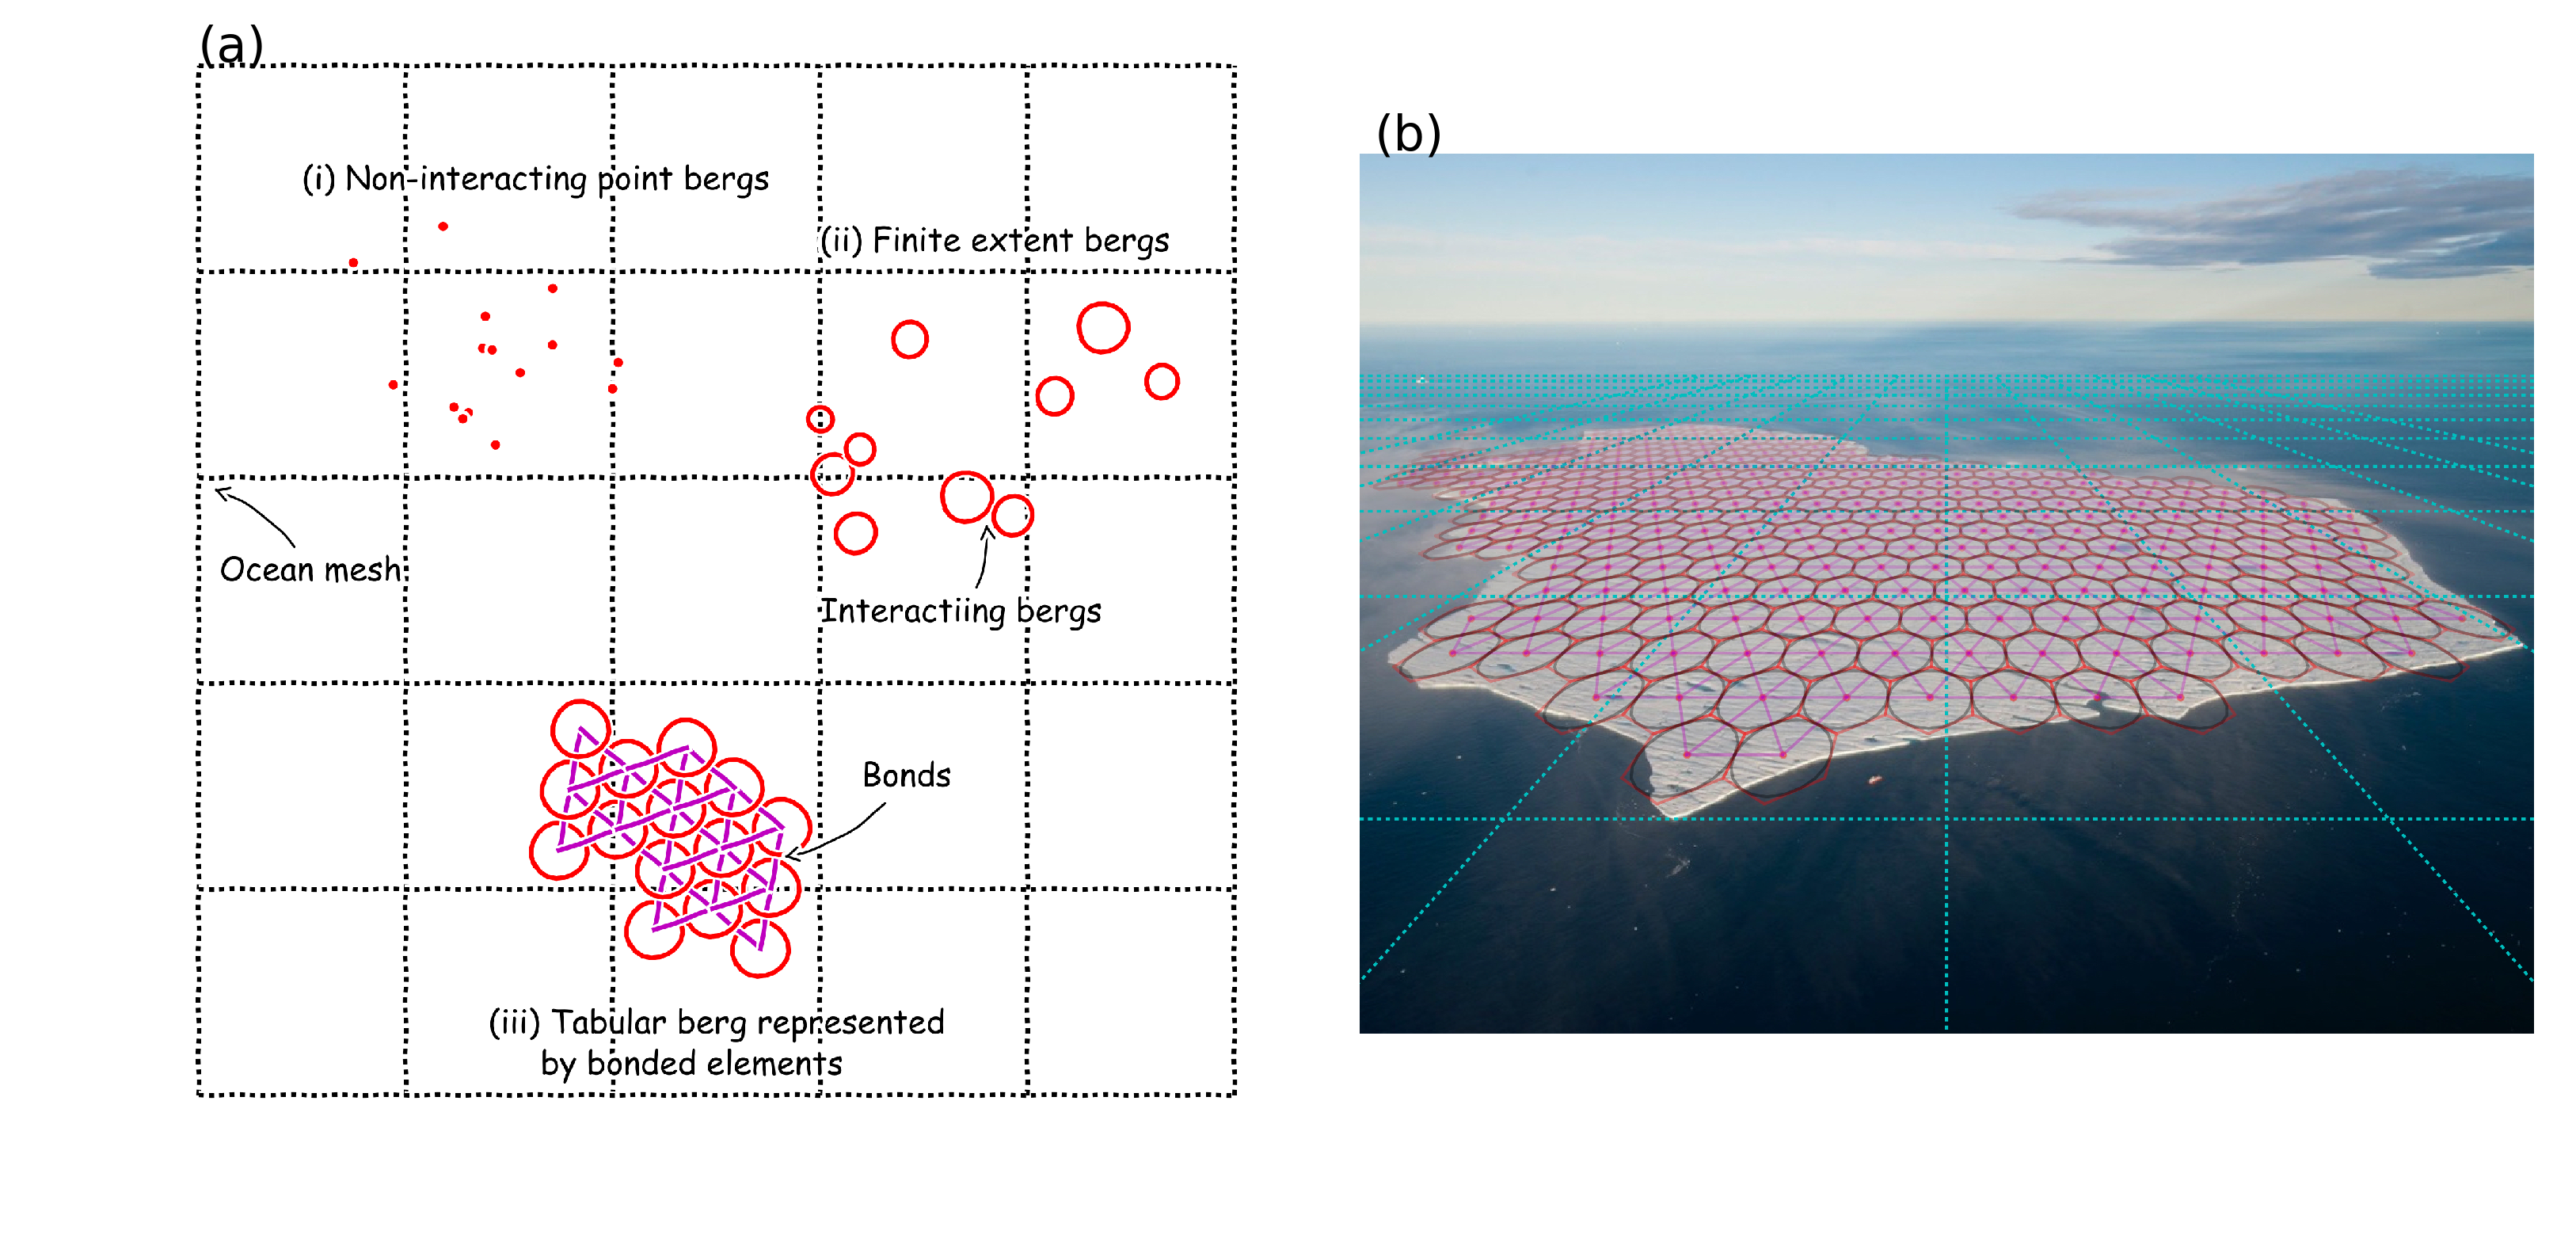
\includegraphics[width=0.99\textwidth]{/Users/alon/Desktop/files/Icebergs_clusters/Towards_Publication/Tech_paper/Github_stuff/Tech-paper/Figures/Two_panel_schematic_berg.png}
%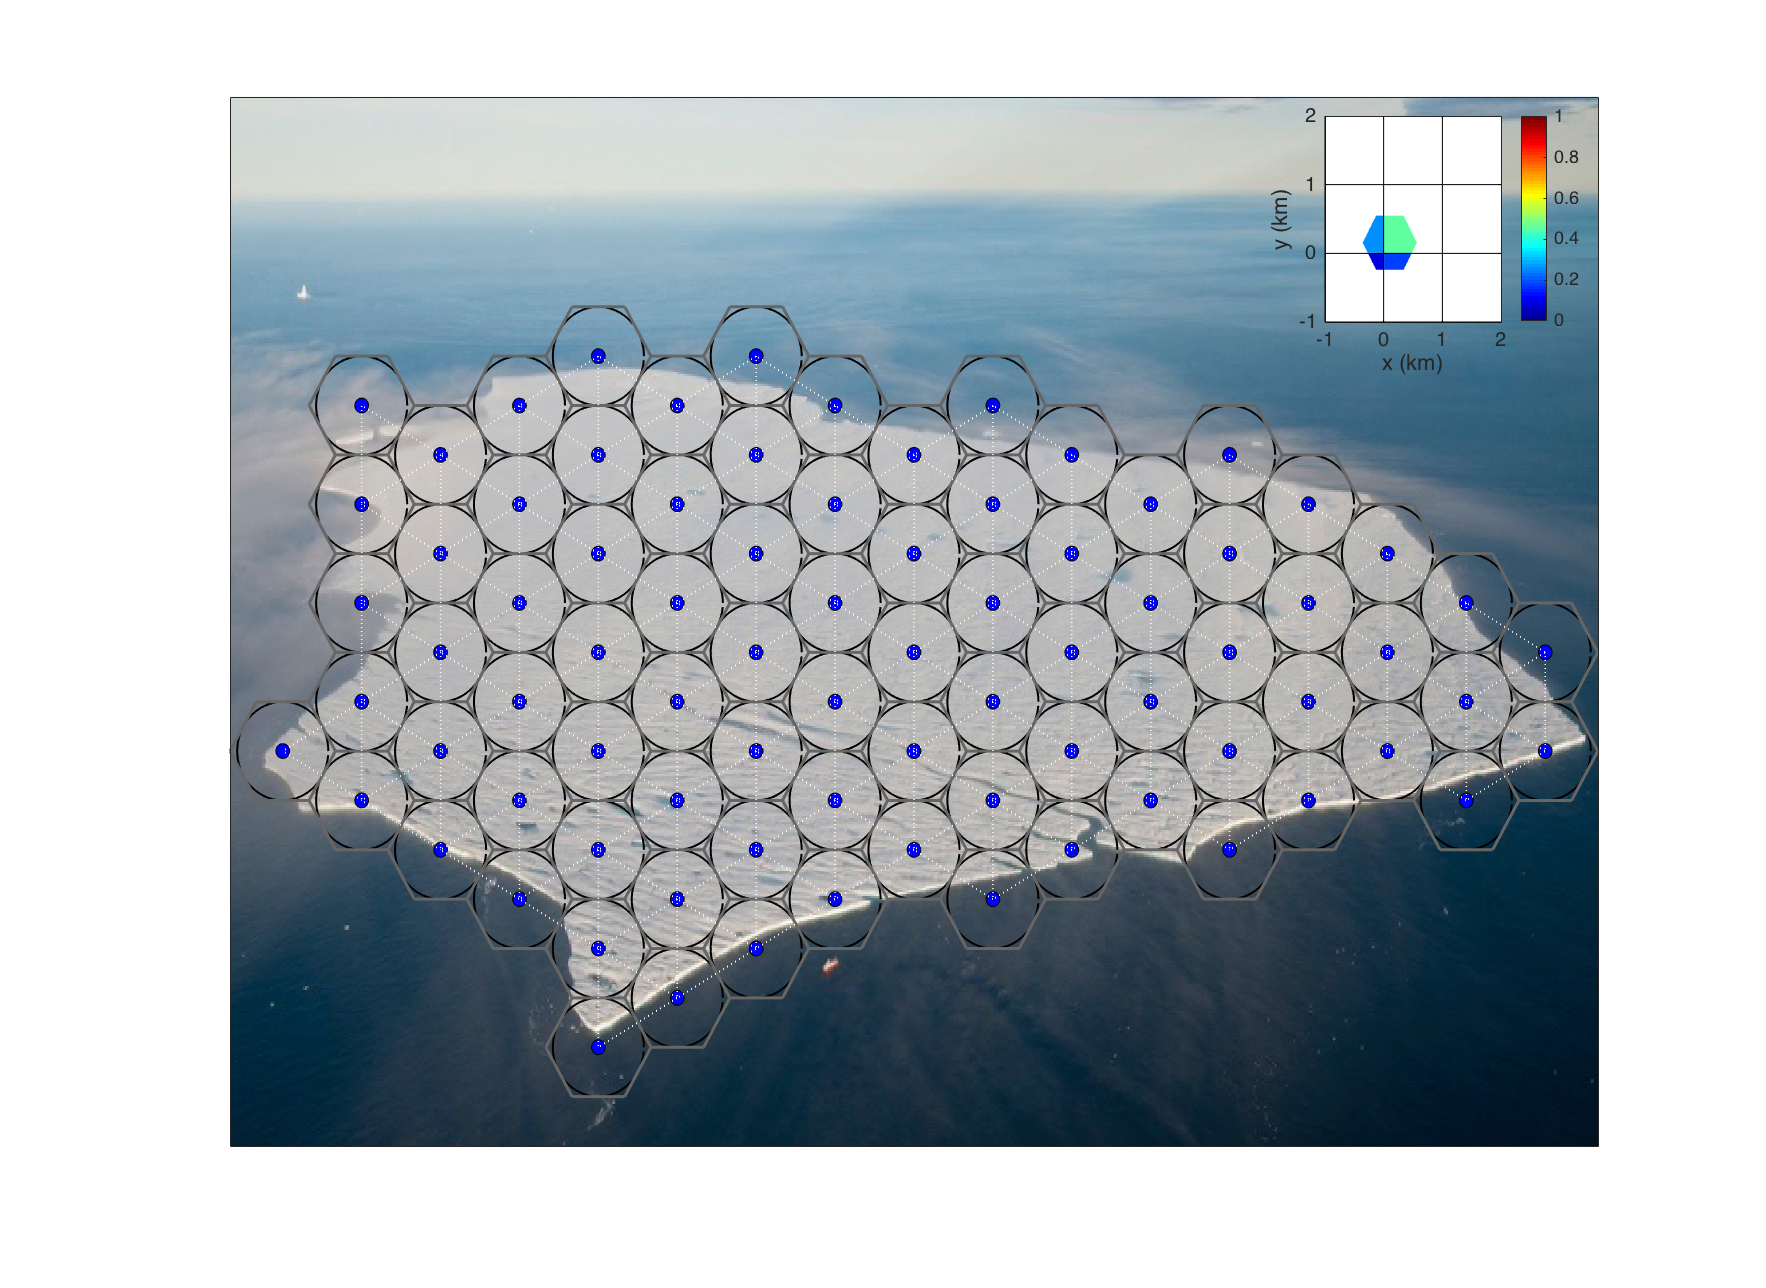
\includegraphics[width=0.99\textwidth]{/Users/alon/Desktop/files/Icebergs_clusters/Towards_Publication/Tech_paper/Github_stuff/Tech-paper/Figures/PIIB_with_hexagons.png}
\caption{Schematic showing how tabular icebergs are constructed using Lagrangian elements. 
(a) Hierarchy of ice elements' physical structure: (i) Previous icebergs models represent icebergs using non-interacting point-particle elements; (ii) In the new framework ice elements are given finite extent so that they are able to interact with the ocean across multiple grid cells, and can interact with other elements; (iii) These finite extent elements can be join together by numerical bonds (magenta lines) to form larger structures such as tabular icebergs.
 (b) Areal photograph of a tabular iceberg with elements superimposed over it to illustrate how the Lagrangian elements can be used to model tabular icebergs. In this schematic the ice elements (purple dots) are initialized in a staggered lattice covering the surface area of the iceberg. For purposed of mass aggregation, the ice elements are assumed to have hexagonal shape (red hexagons). For purposed of element interactions, the ice elements are assumed to be circular (black circles). Elements are initially bonded to adjacent elements using numerical bonds (magenta lines). These numerical bonds form equilateral triangles which give the shape rigidity. An ocean grid has been included (dashed cyan lines). %The background photo in the larger schematic is an areal photograph of iceberg PIIB (Area= 42 $\textrm{km}^{2}$) taken in Baffin Bay in 2012. The red ship can be identified on the bottom of the photo for scale. 
%Schematic showing how Lagrangian elements are used when modeling tabular icebergs. Lagrangian elements (blue dots) are initialized in a staggered lattice covering the surface area of the iceberg. For purposed of mass aggregation, the ice elements are assumed to have hexagonal shape (grey hexagons). For purposed of element interactions, the ice elements are assumed to be circular (black circles). Elements are initially bonded to adjacent elements using numerical bonds (dashed white lines). These numerical bonds form equilateral triangles which give the shape rigidity. 
%The inset panel shows a schematic of the intersection of a hexagonal element and the ocean grid. The colors indicate the fraction of the hexagon that lies in each grid cell. These fractions are used as weights to spread iceberg model properties to the ocean grid (see text for more details).
The background photo is an areal photograph of iceberg PIIB (Area= 42 $\textrm{km}^{2}$) taken in Baffin Bay in 2012. A red ship can be identified on the bottom of the photo for scale. \label{fig:Hex_schematic}}
\end{center}

\end{figure}
 \clearpage


%\begin{figure}
%\begin{center}
%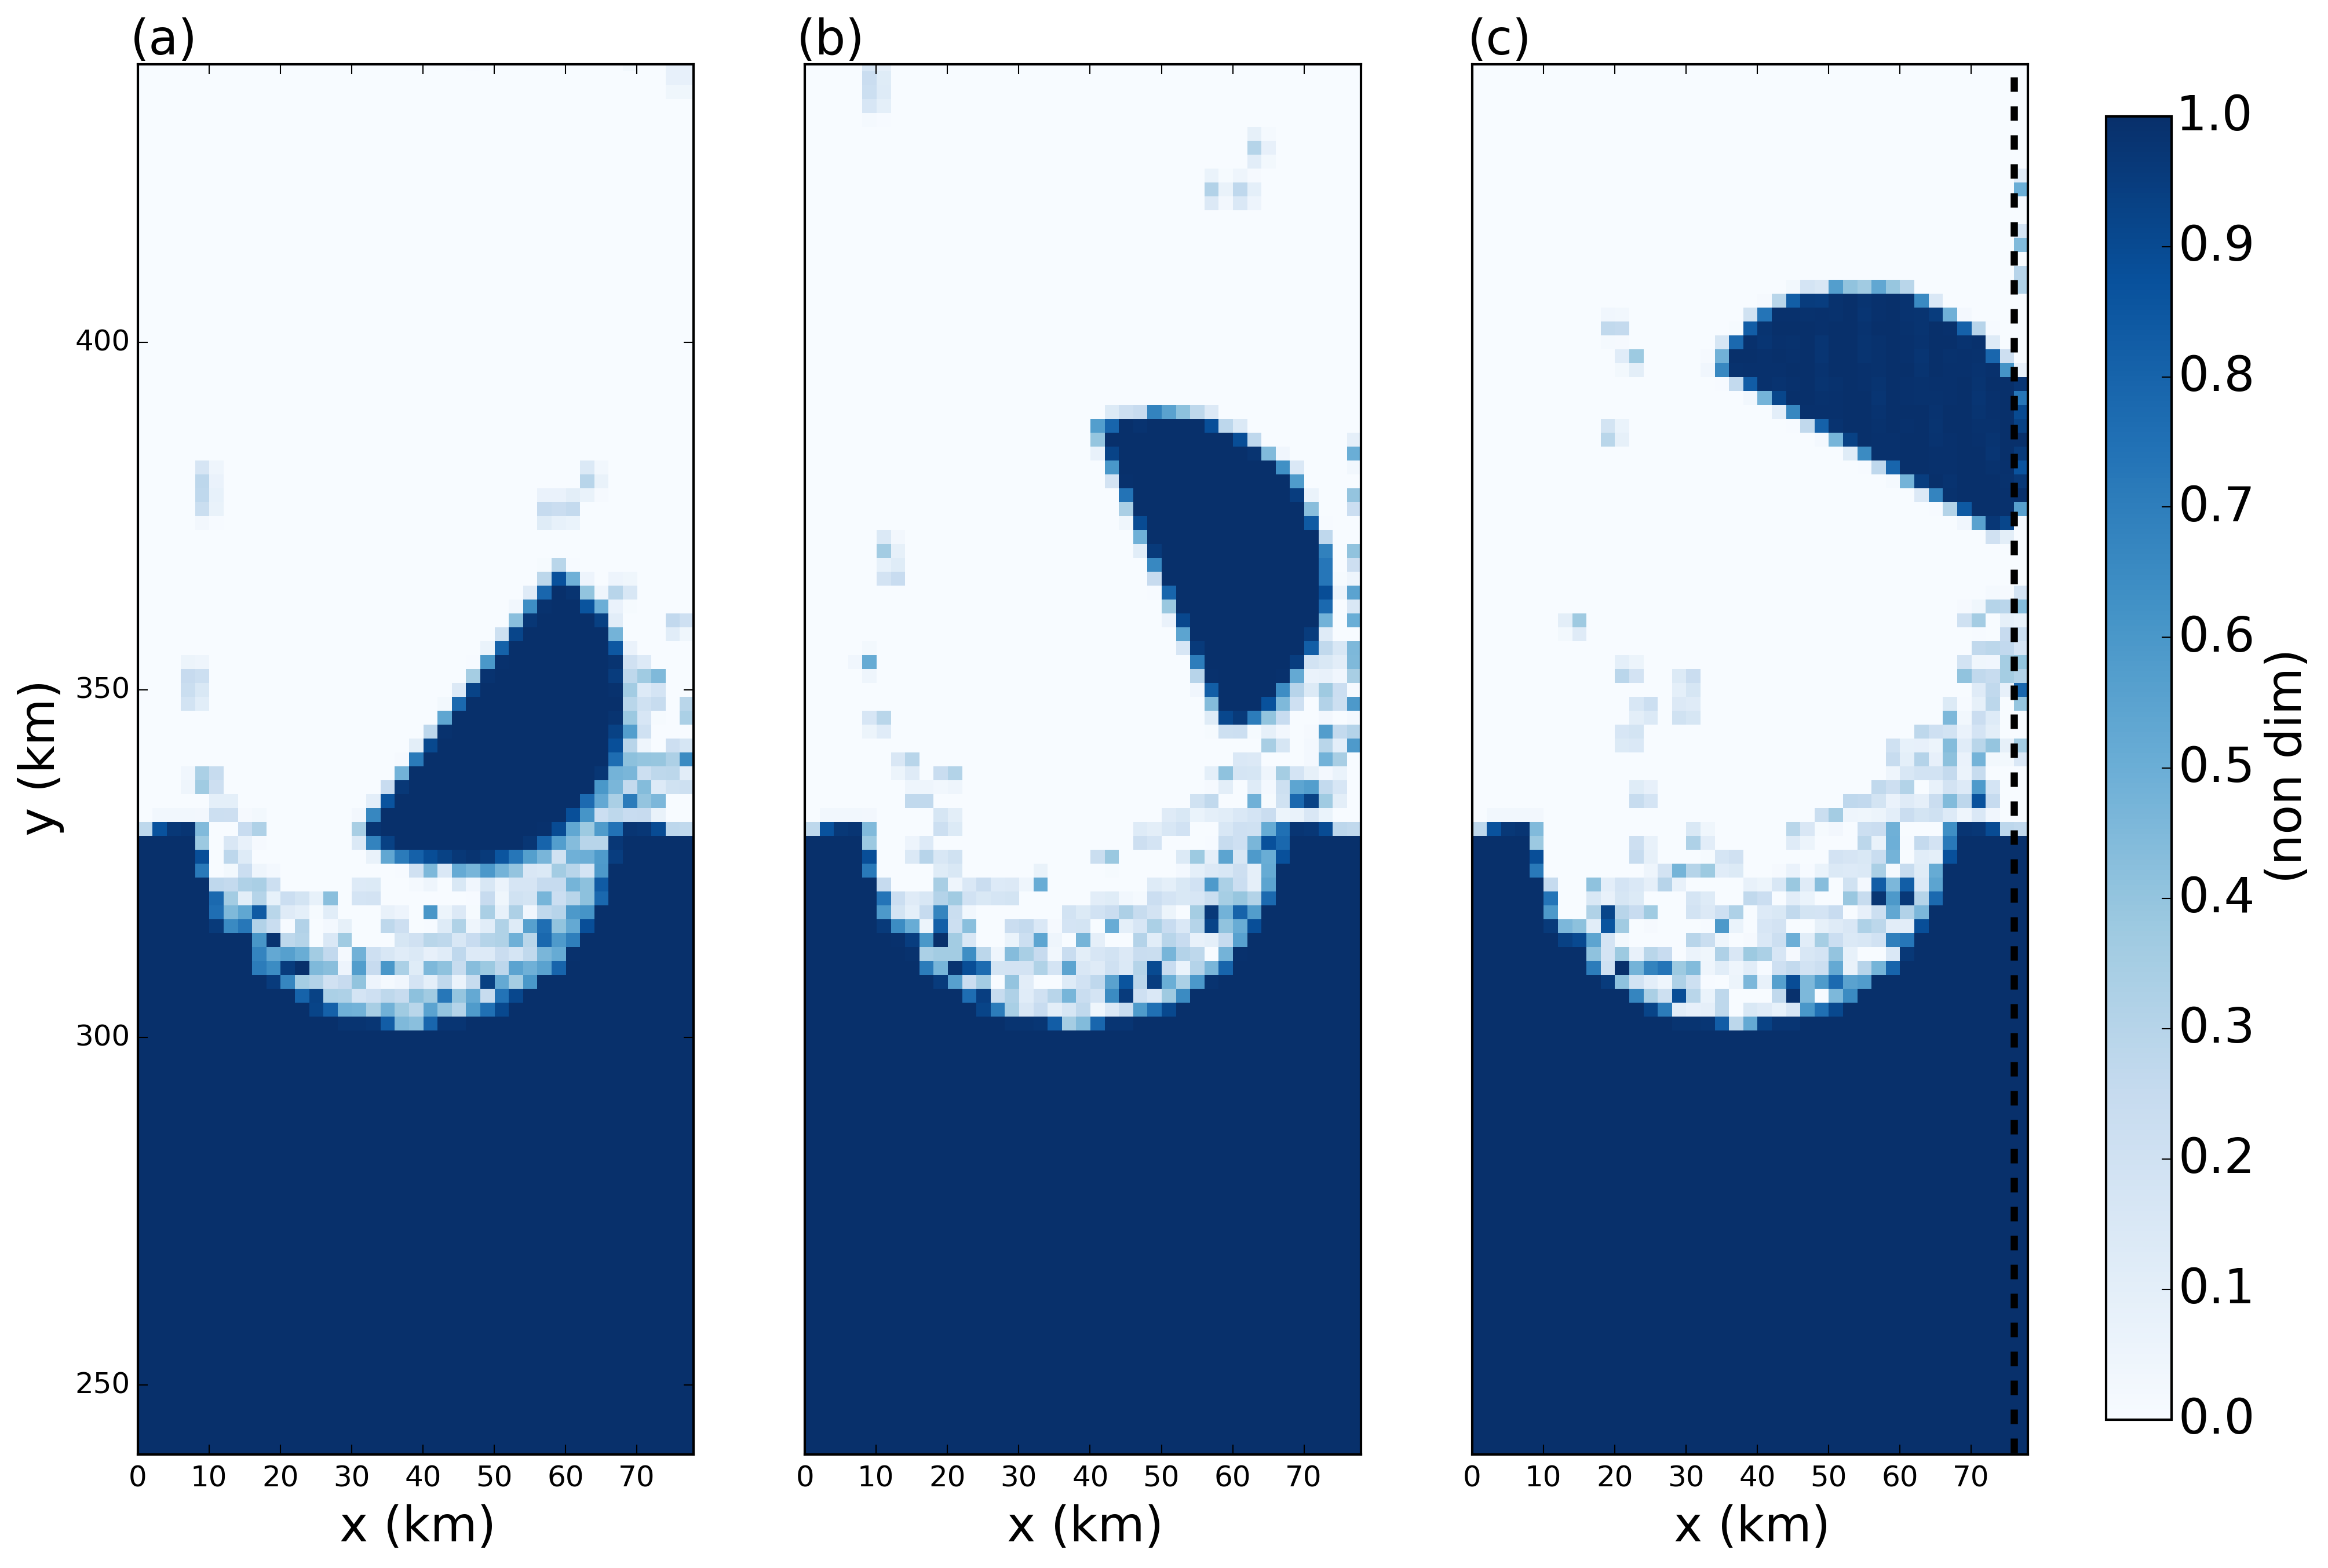
\includegraphics[width=0.99\textwidth]{/Users/alon/Desktop/files/Icebergs_clusters/Towards_Publication/Tech_paper/Github_stuff/Tech-paper/Figures/snapshots_ALE_z_Mixed_Melt_Collapse_spread_area.png}
%\caption{ {Snapshots of the fraction of ice cover in the iceberg model tabular iceberg calving simulation. Snapshots are taken (a) 7, (b) 15, and (c) 30 days after calving. The dashed line in panel (c) shows the location of the vertical transects shown in Figures \ref{fig:Velocity_section_Collapse} and \ref{fig:Temperature_section_Collapse}}. \label{fig:Spread_area}}
%\end{center}
%\end{figure}
 %\clearpage



\begin{figure}
\begin{center}
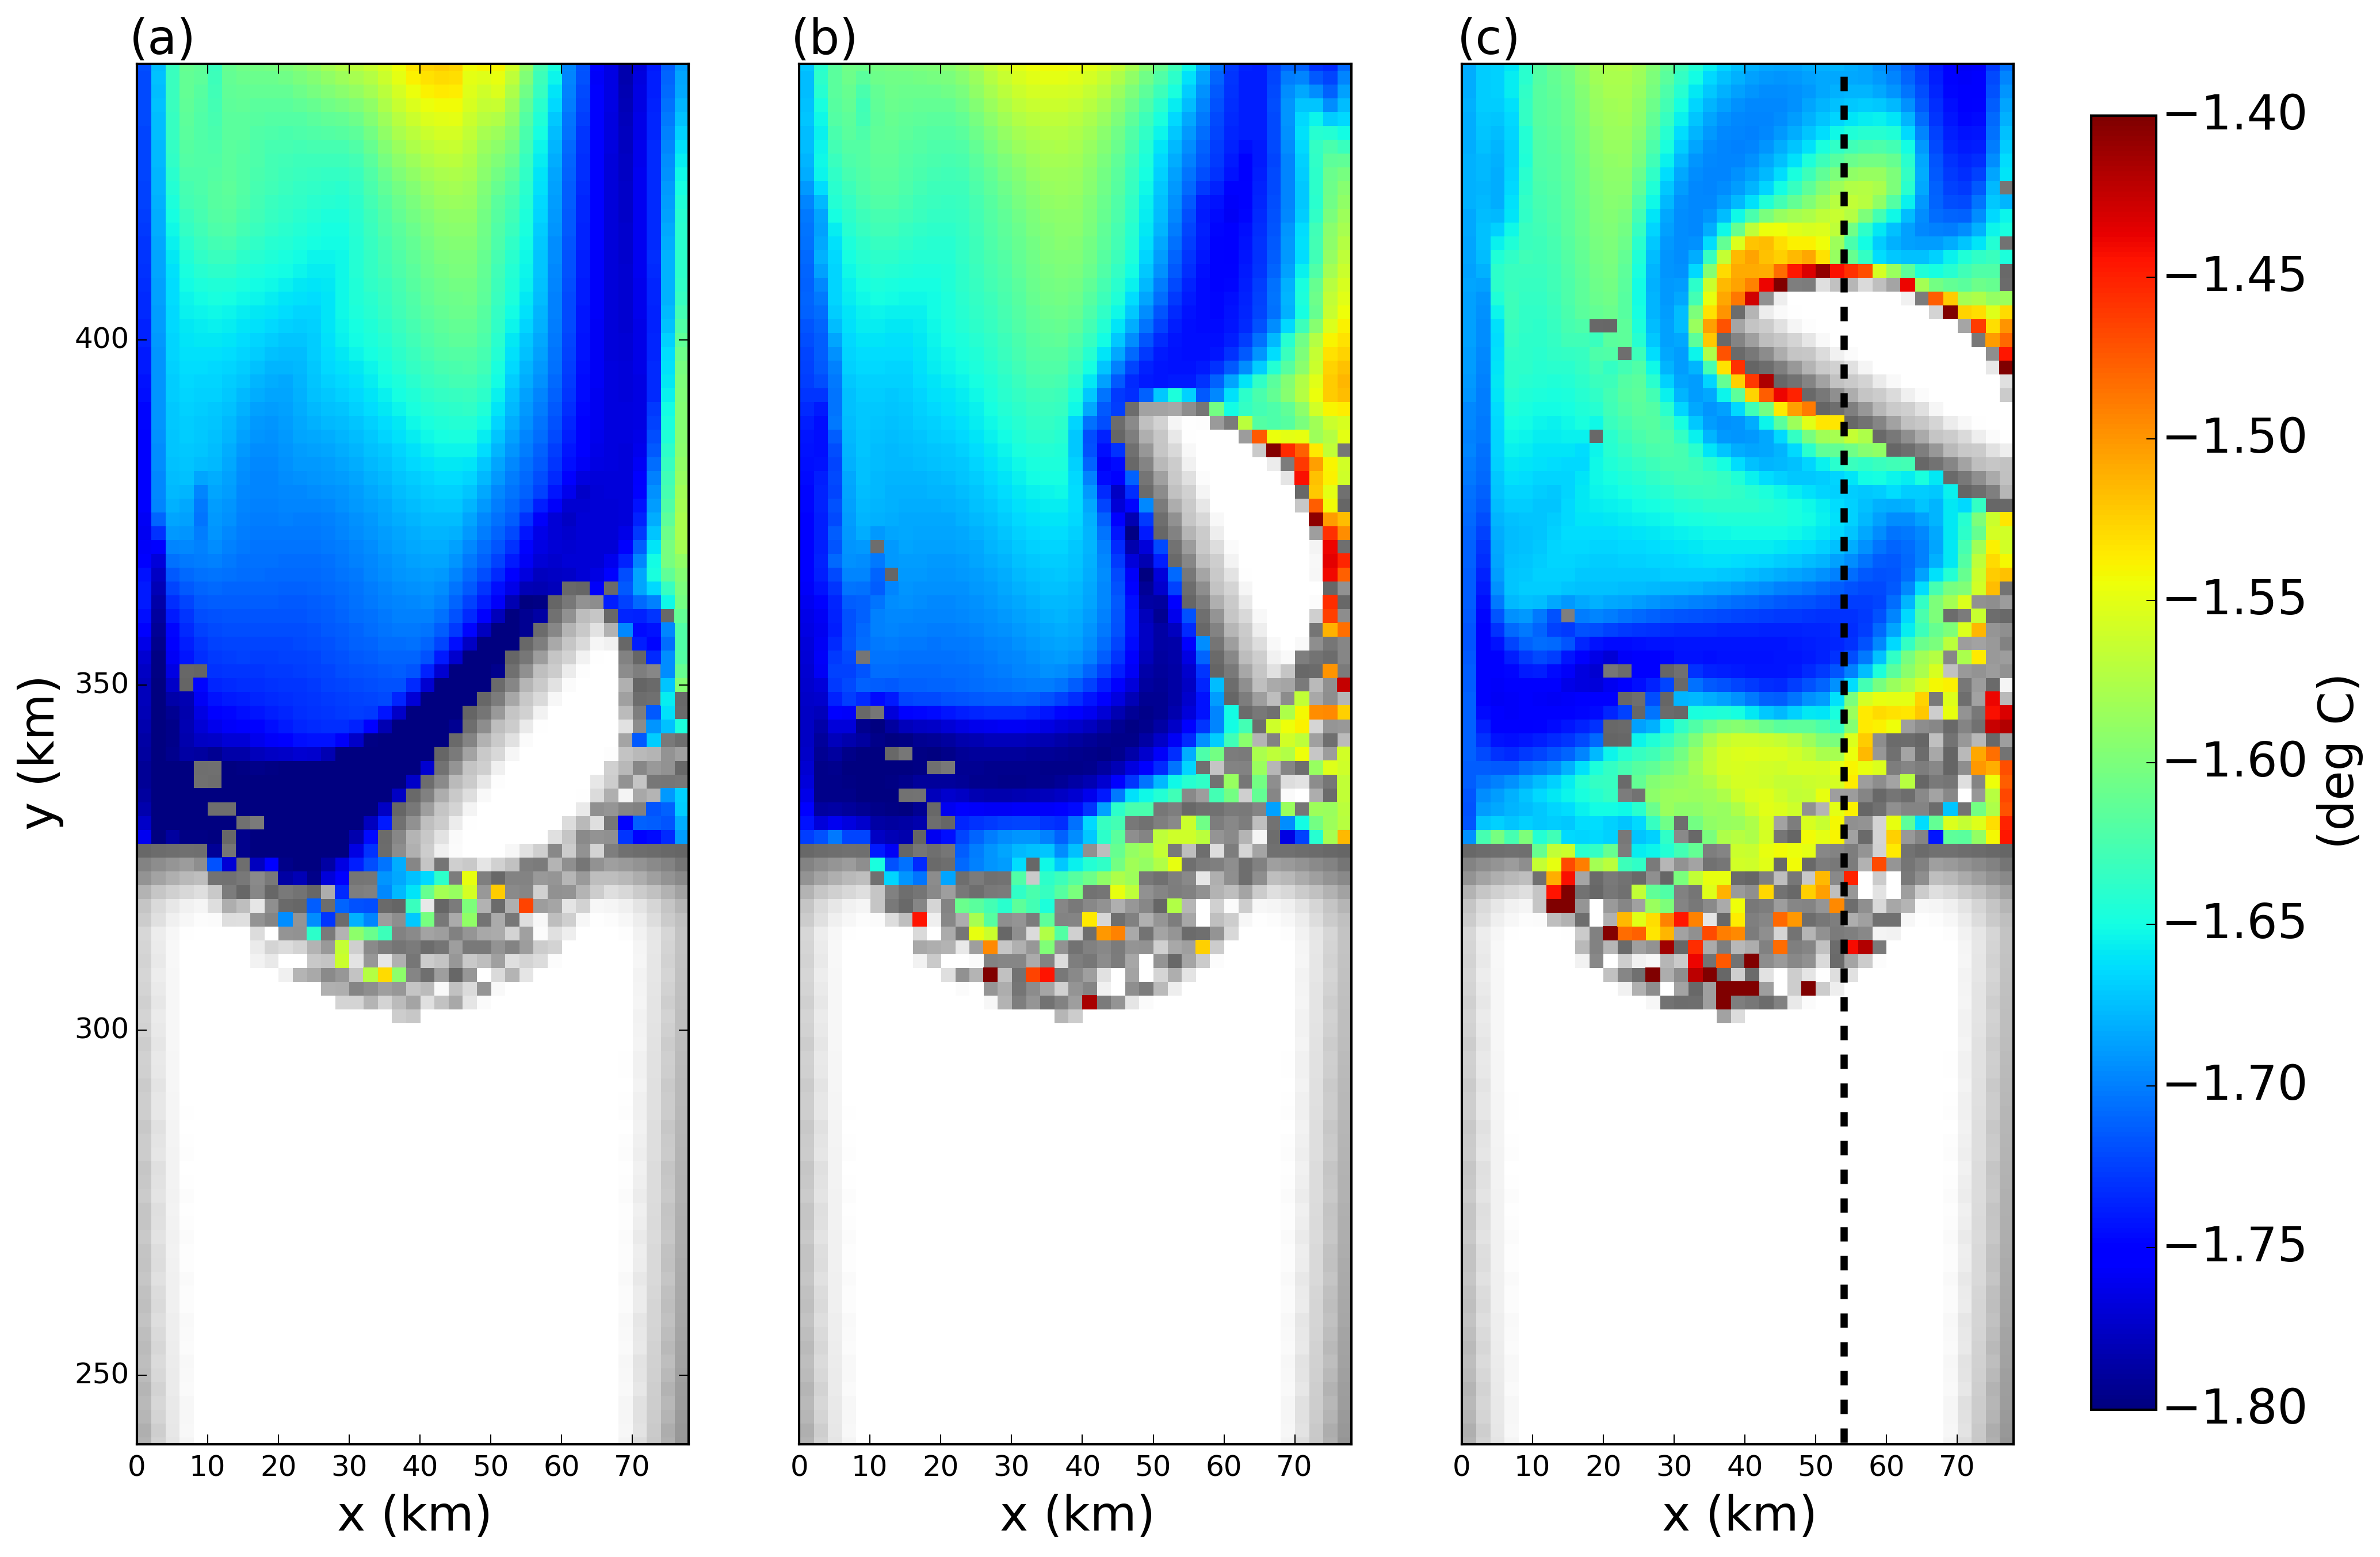
\includegraphics[width=0.99\textwidth]{/Users/alon/Desktop/files/Icebergs_clusters/Towards_Publication/Tech_paper/Github_stuff/Tech-paper/Figures/snapshots_ALE_z_Mixed_Melt_Collapse_temp.png}
\caption{ {Snapshots of the sea surface temperature in the tabular iceberg calving simulation. Snapshots are taken (a) 7, (b) 15, and (c) 30 days after calving. Grid cells with ice mass > $10^{4}$ kg are plotted in white, with grey shading indicating thinner ice.  The dashed line in panel (c) shows the location of the vertical transects shown in Figures \ref{fig:Temperature_section_Collapse} and \ref{fig:Velocity_section_Collapse}.} 
\label{fig:SST_Collapse}}
\end{center}
\end{figure}
 \clearpage


\begin{figure}
\begin{center}
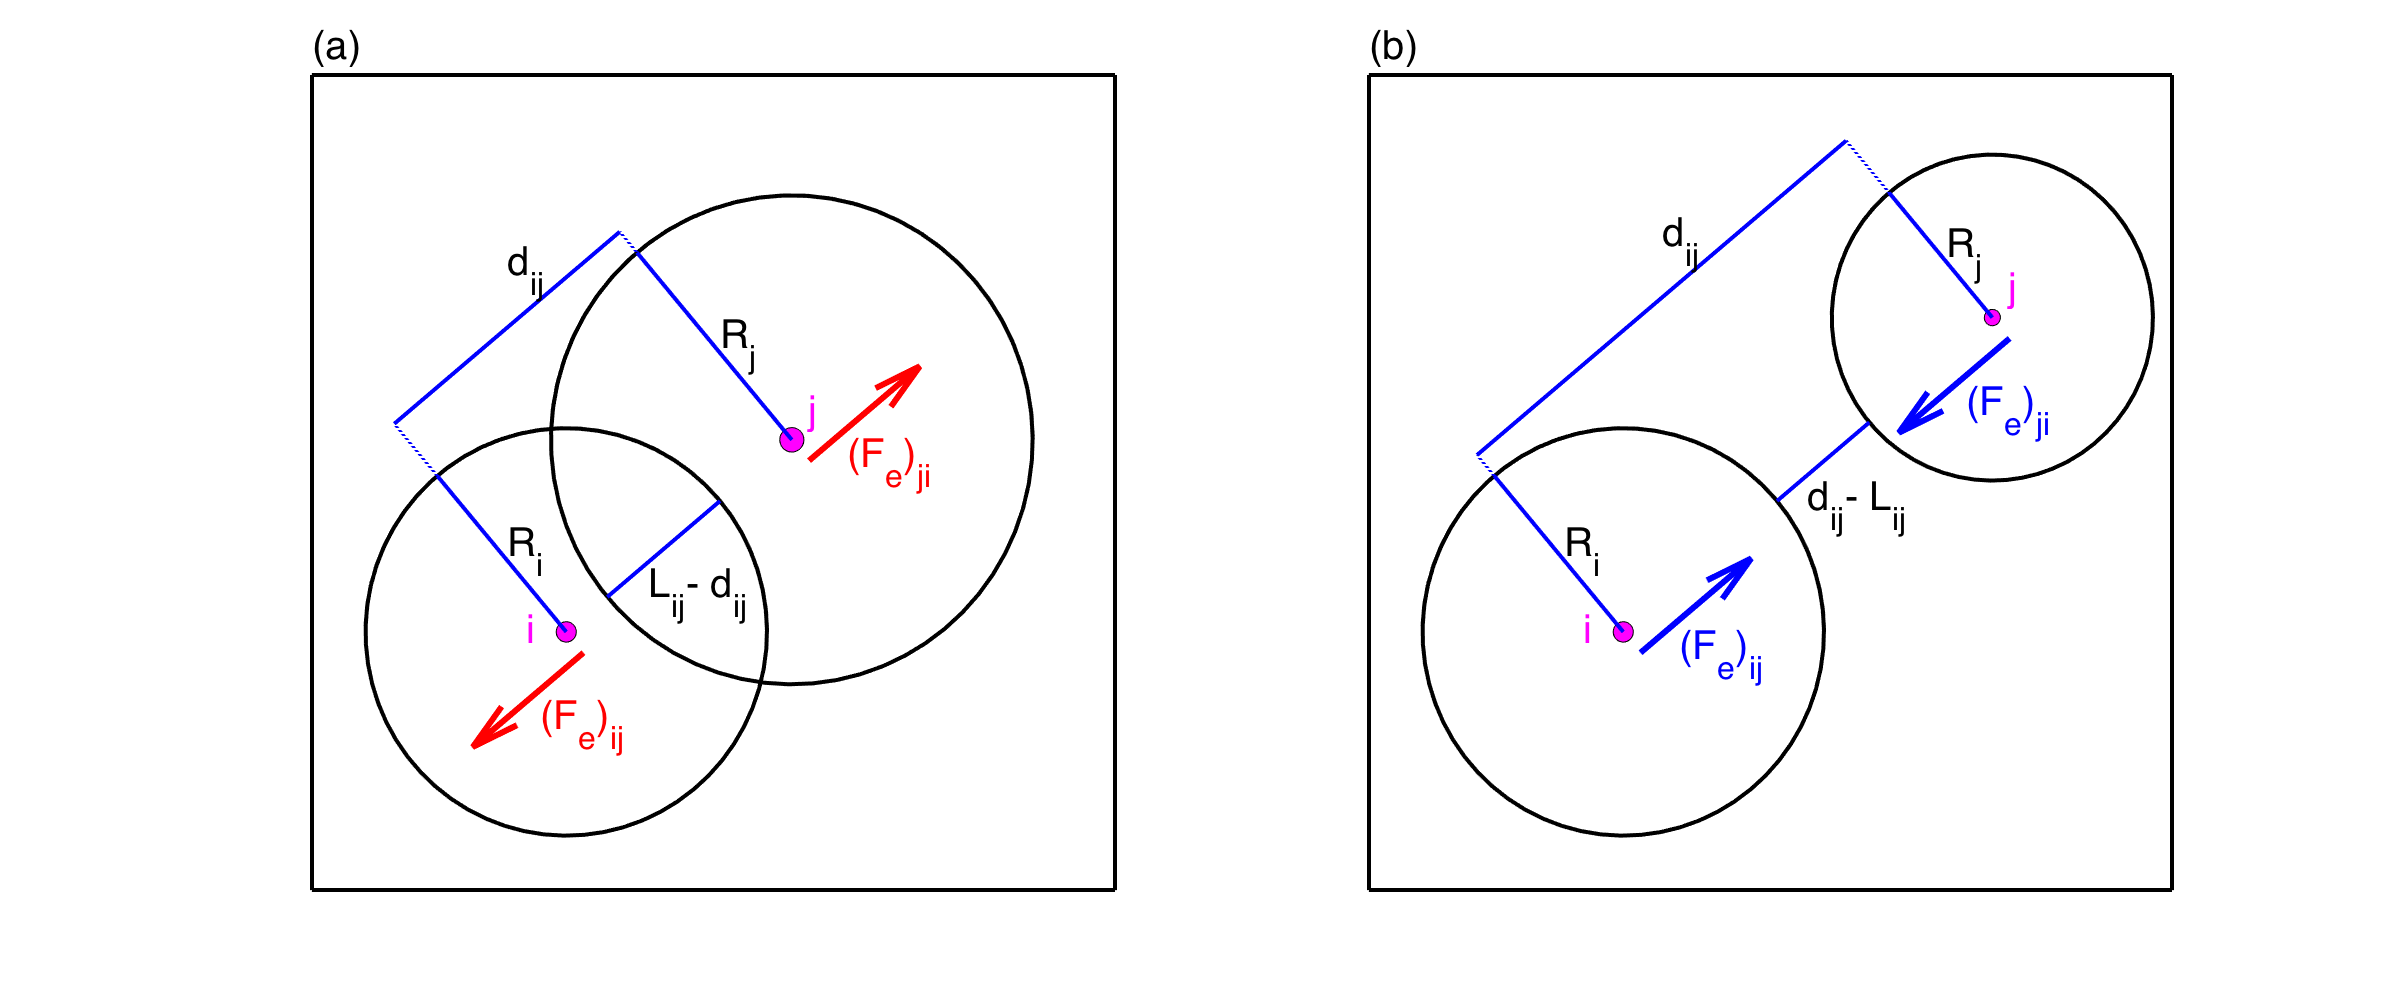
\includegraphics[width=0.99\textwidth]{/Users/alon/Desktop/files/Icebergs_clusters/Towards_Publication/Tech_paper/Github_stuff/Tech-paper/Figures/interactive_force_diagram}
%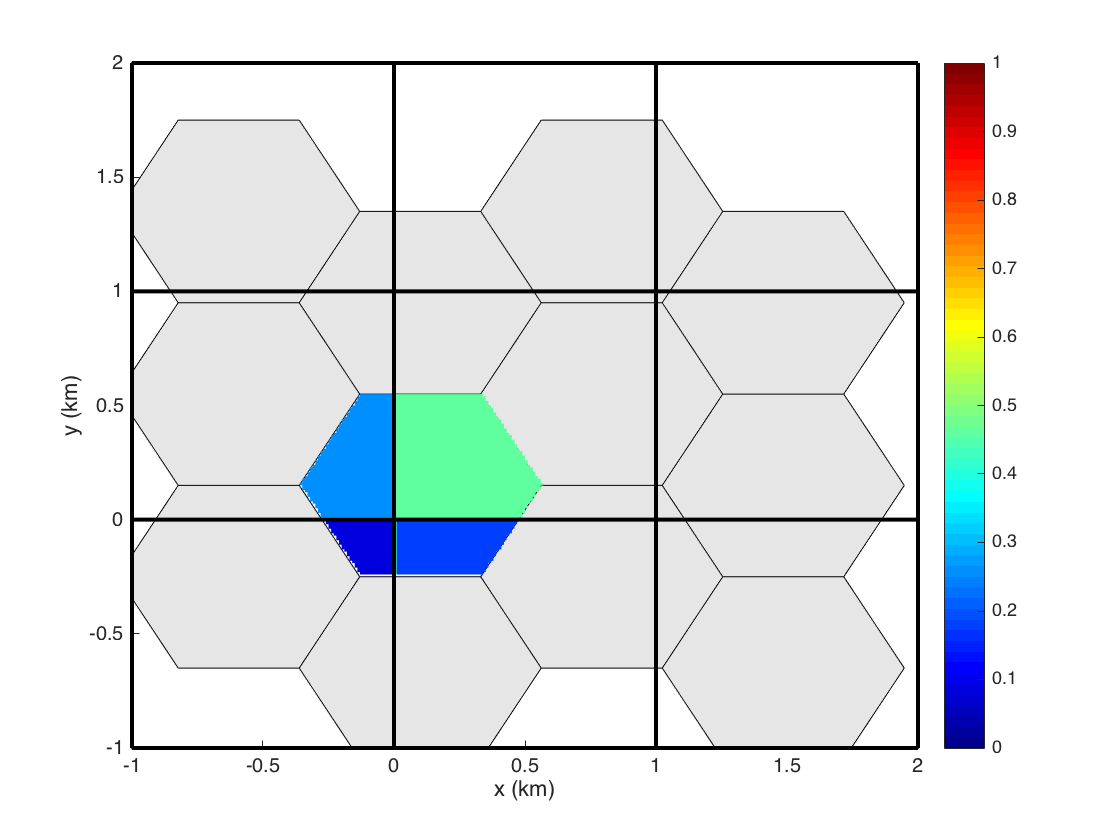
\includegraphics[width=0.69\textwidth]{/Users/alon/Desktop/files/Icebergs_clusters/Towards_Publication/Tech_paper/Github_stuff/Tech-paper/Figures/hex_on_a_grid}
\caption{ { Diagram showing the (a) repulsive and (b) attractive elastic interactive forces between two elements, $i$ and $j$.  $R_{i}$ and $R_{j}$ are the interactive radii of element $i$ and $j$, respectively. $d_{ij}$ is the distance between the centers of elements. $L_{i,j}=R_{i}+R_{j}$ is the critical-interactive-length scale. $(F_{e})_{ij}$ and $(F_{e})_{ji}$ are the elastic forces applied to elements $i$ and $j$, respectively (equation \ref{F_elastic}).  A frictional damping force is also applied, which opposes the relative velocity of the elements (not shown). The attractive forces are only applied when the two elements are bonded together (i.e.: $B_{ij}=1$).}
\label{fig:Force_diagram}}
\end{center}

\end{figure}
\clearpage




\begin{figure}
\begin{center}
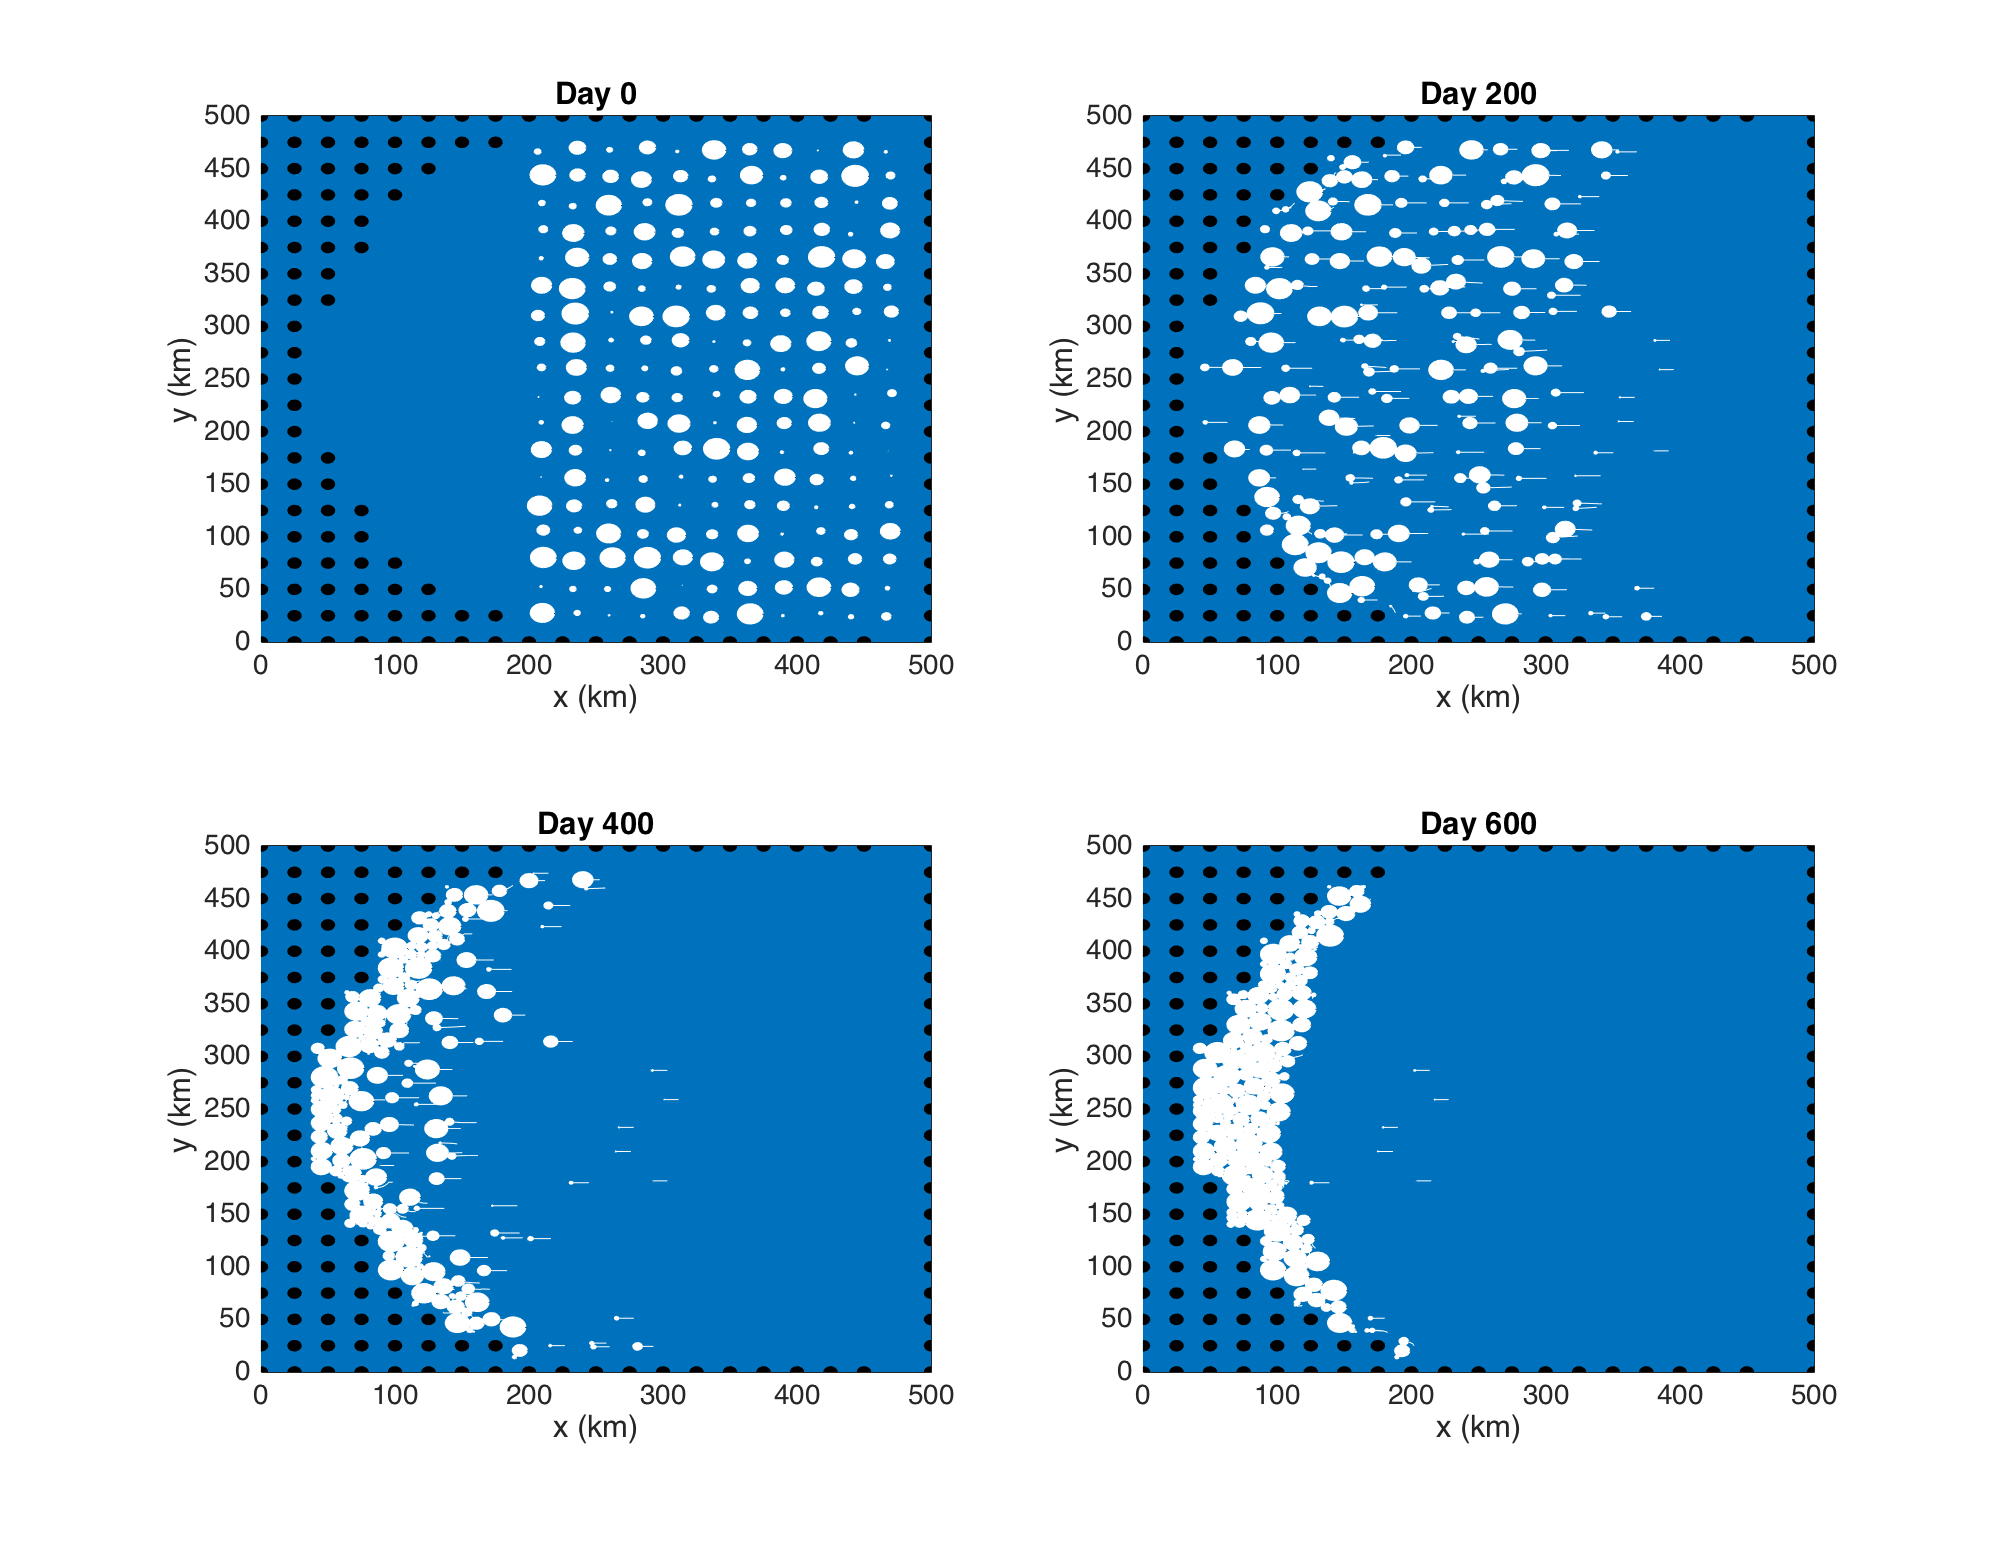
\includegraphics[width=0.99\textwidth]{/Users/alon/Desktop/files/Icebergs_clusters/Towards_Publication/Tech_paper/Github_stuff/Tech-paper/Figures/Regular_towards_coast_tails.png}
\caption{ {Results of an uncoupled (ice-only) simulation with no bonds between ice elements. Ice elements are initialized throughout the domain, as shown in top left panel. The elements are forced by an imposed westward ocean current of u=0.1m/s (no ocean model is used). Forces due to sea surface slope, atmospheric drag, Coriolis and sea ice drag are set to zero. The figure shows snapshots of ice element positions at time t=0, 17, 33 and 50 days. The size of the dots shows the surface area (and interaction radius) of each ice element. The white tails behind the elements show the elements' positions over the preceding two days. Land points are shown by black circles.}\label{fig:Regular_Uncoupled_sim}}
\end{center}
\end{figure}
 \clearpage


\begin{figure}
\begin{center}
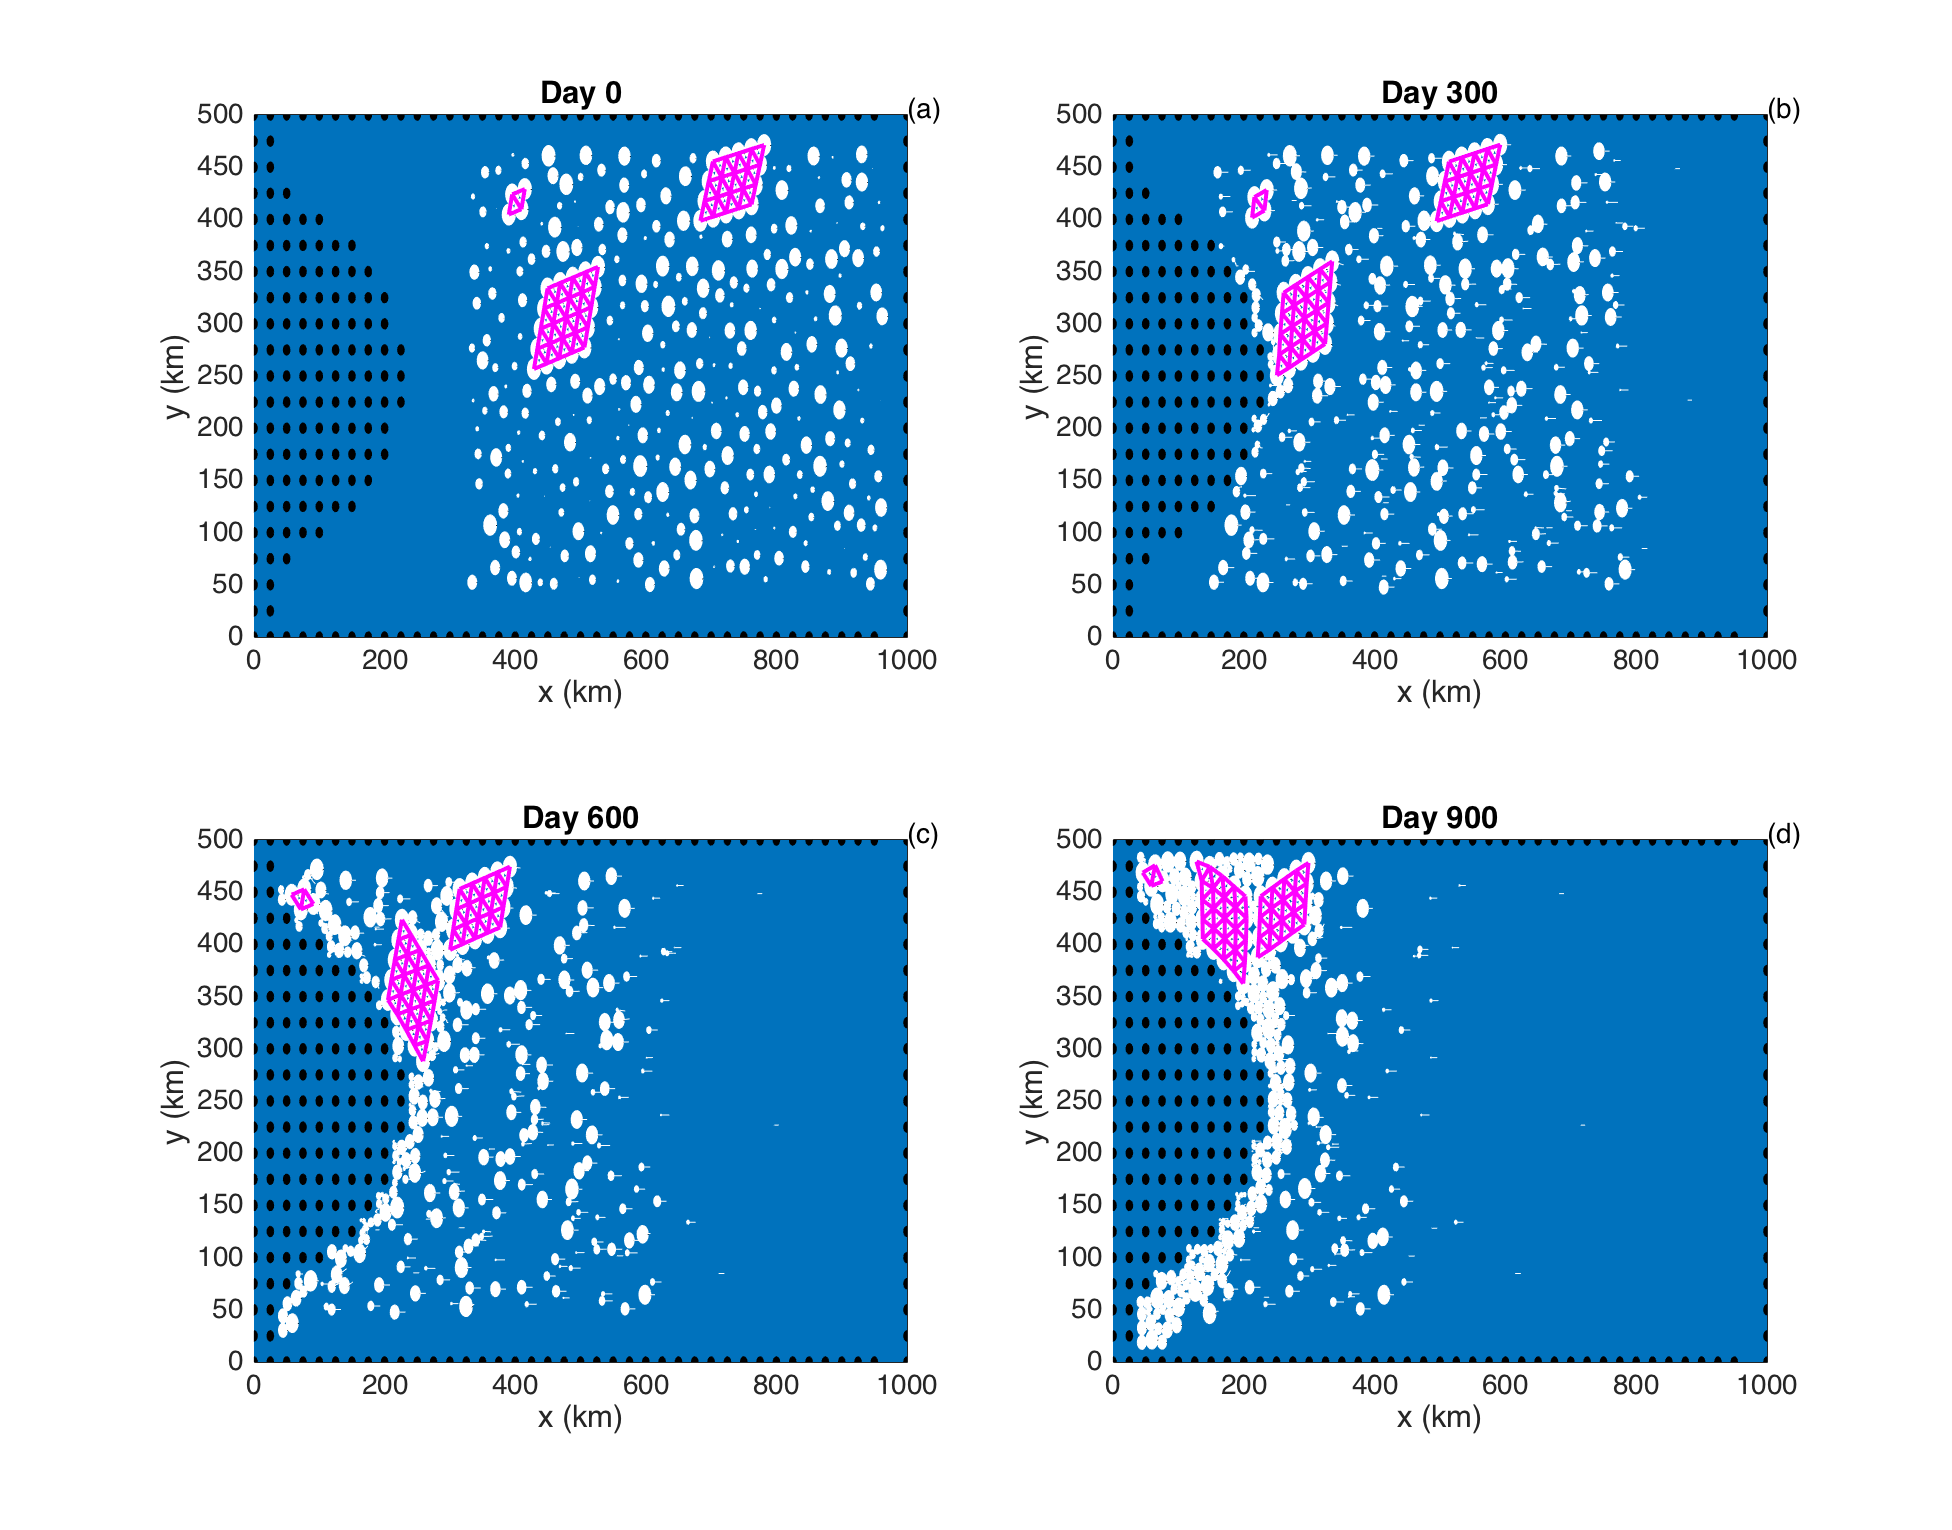
\includegraphics[width=0.99\textwidth]{/Users/alon/Desktop/files/Icebergs_clusters/Towards_Publication/Tech_paper/Github_stuff/Tech-paper/Figures/Tabular_and_regular_towards_coast_manual_tails.png}
\caption{ {Results of an uncoupled (ice-only) simulation using bonds between elements. Ice elements are initialized throughout the domain, as shown in top left panel. Three tabular icebergs are included, with 25, 16 and 4 elements respectively. The elements are forced by an imposed westward ocean current of u=0.1m/s (no ocean model is used). Forces due to sea surface slope, atmospheric drag, Coriolis and sea ice drag are set to zero. The figure shows snapshots of ice element positions at time t=0, 25, 52, and 75 days. The size of the dots shows the surface area (and interaction radius) of each ice element. The white tails behind the elements show the elements' positions over the preceding two days. Bonds between ice elements are plotted in magenta. Land points are shown by black circles.} \label{fig:Uncoupled_sim}}
\end{center}
\end{figure}
 \clearpage



%\begin{figure}
%\begin{center}
%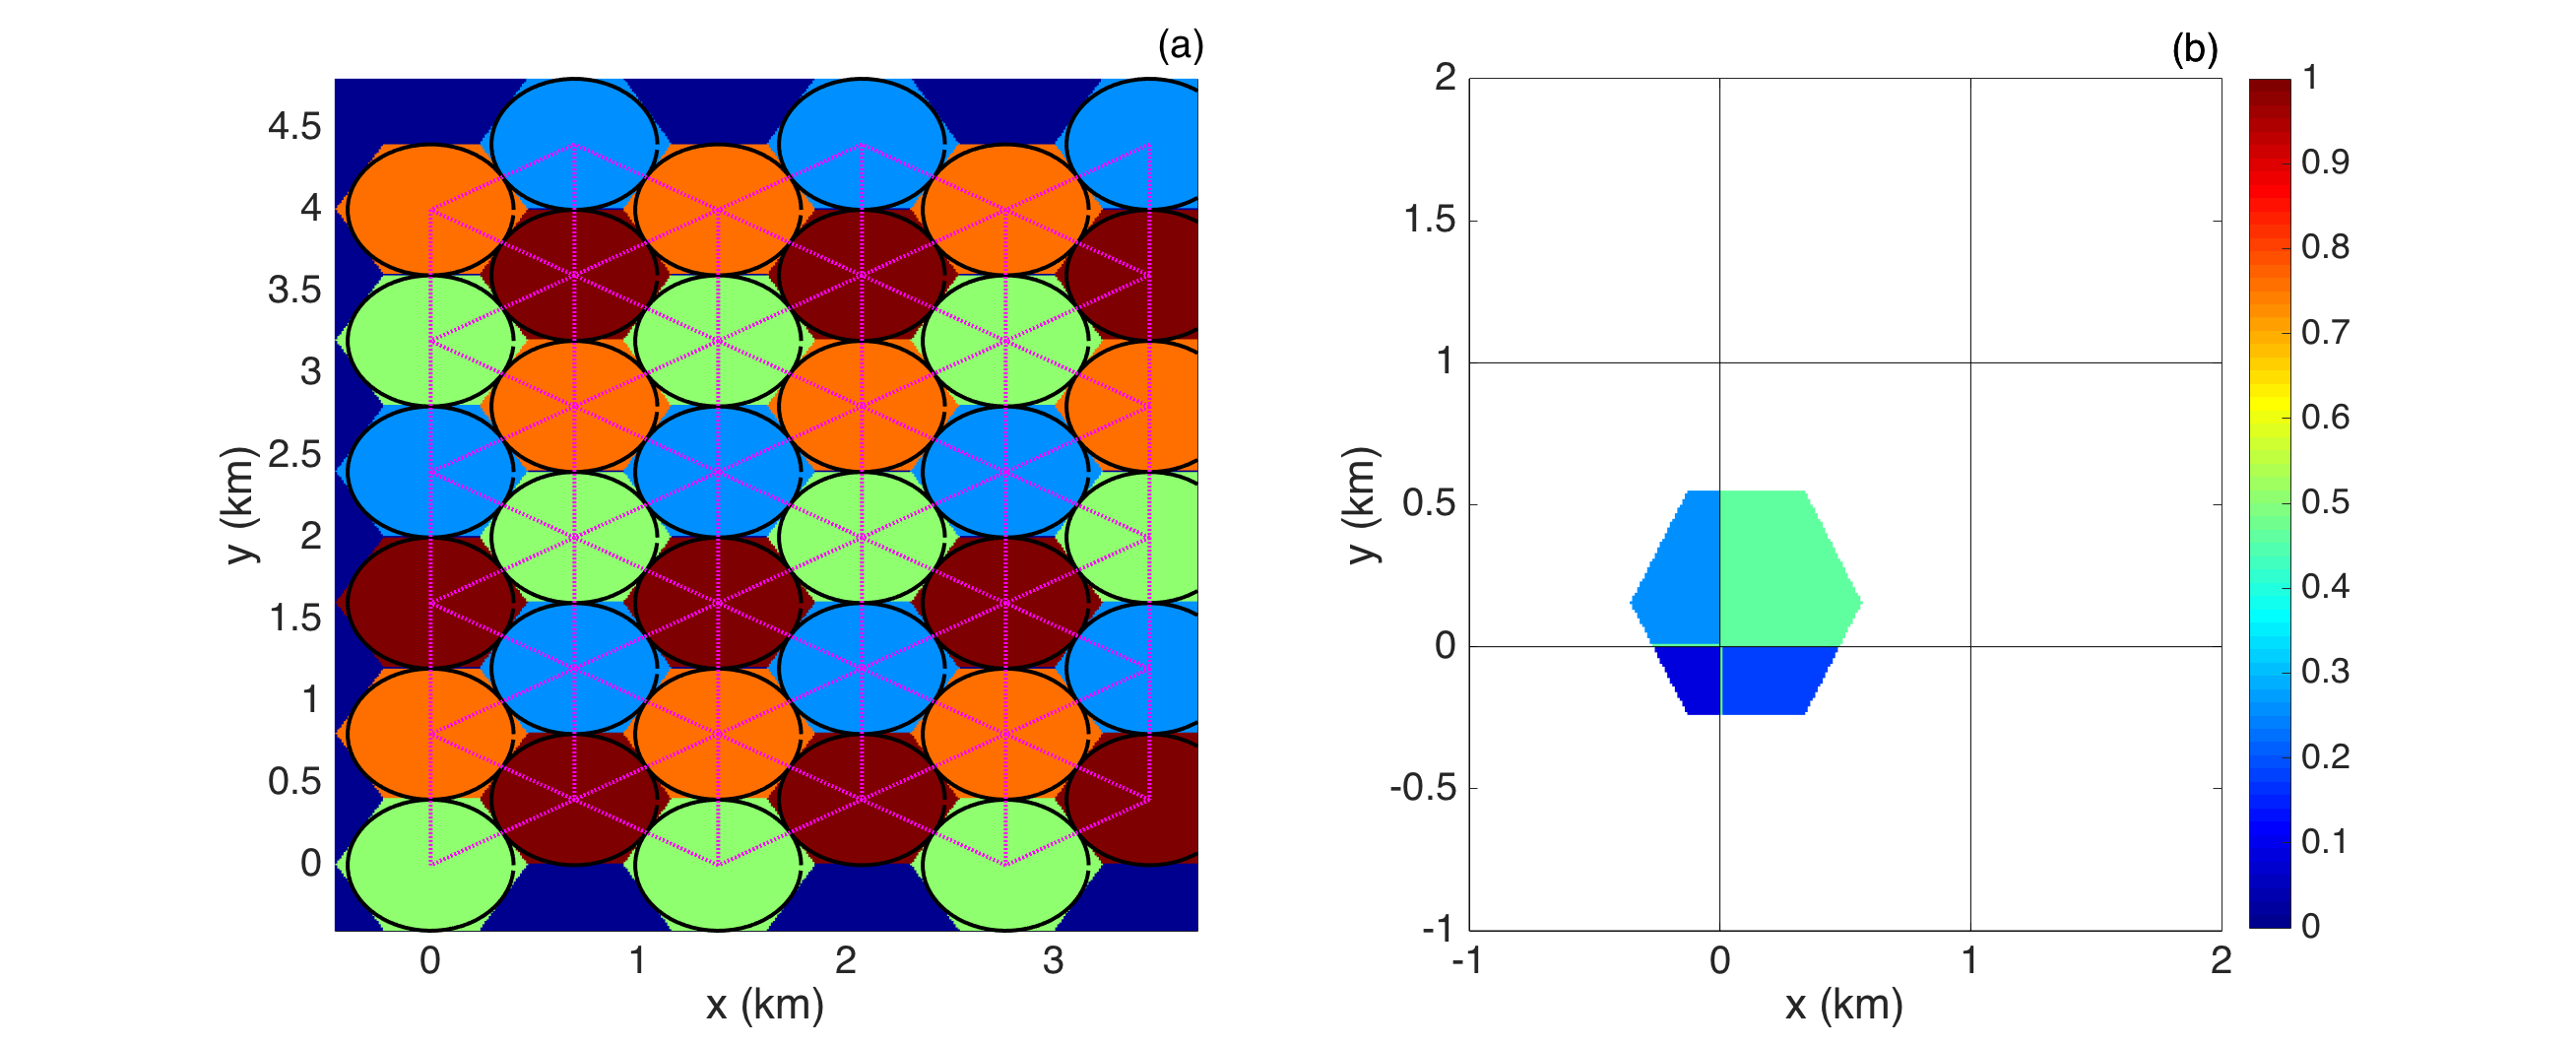
\includegraphics[width=0.99\textwidth]{/Users/alon/Desktop/files/Icebergs_clusters/Towards_Publication/Tech_paper/Github_stuff/Tech-paper/Figures/hex_intersecting_rectangles}
%\caption{ {(a) Hexagonal elements are initialized in a staggered lattice as shown. Adjacent elements are bonded together. The element bonds (plotted in pink) form equilateral triangles which give the larger structure rigidity. The black circles show the circular element shape used in element interactions, and are inscribed inside the hexagonal shape used for mass-spreading. (b) Intersection of a hexagonal element and the ocean grid. The colors indicate the fraction of the hexagon that lies in each grid cell. These fractions are used as weights to spread iceberg model properties to the ocean grid (see text for more details).}}
%\end{center}
%\label{fig:Hex_intersections}
%\end{figure}
 %\clearpage




\begin{figure}
\begin{center}
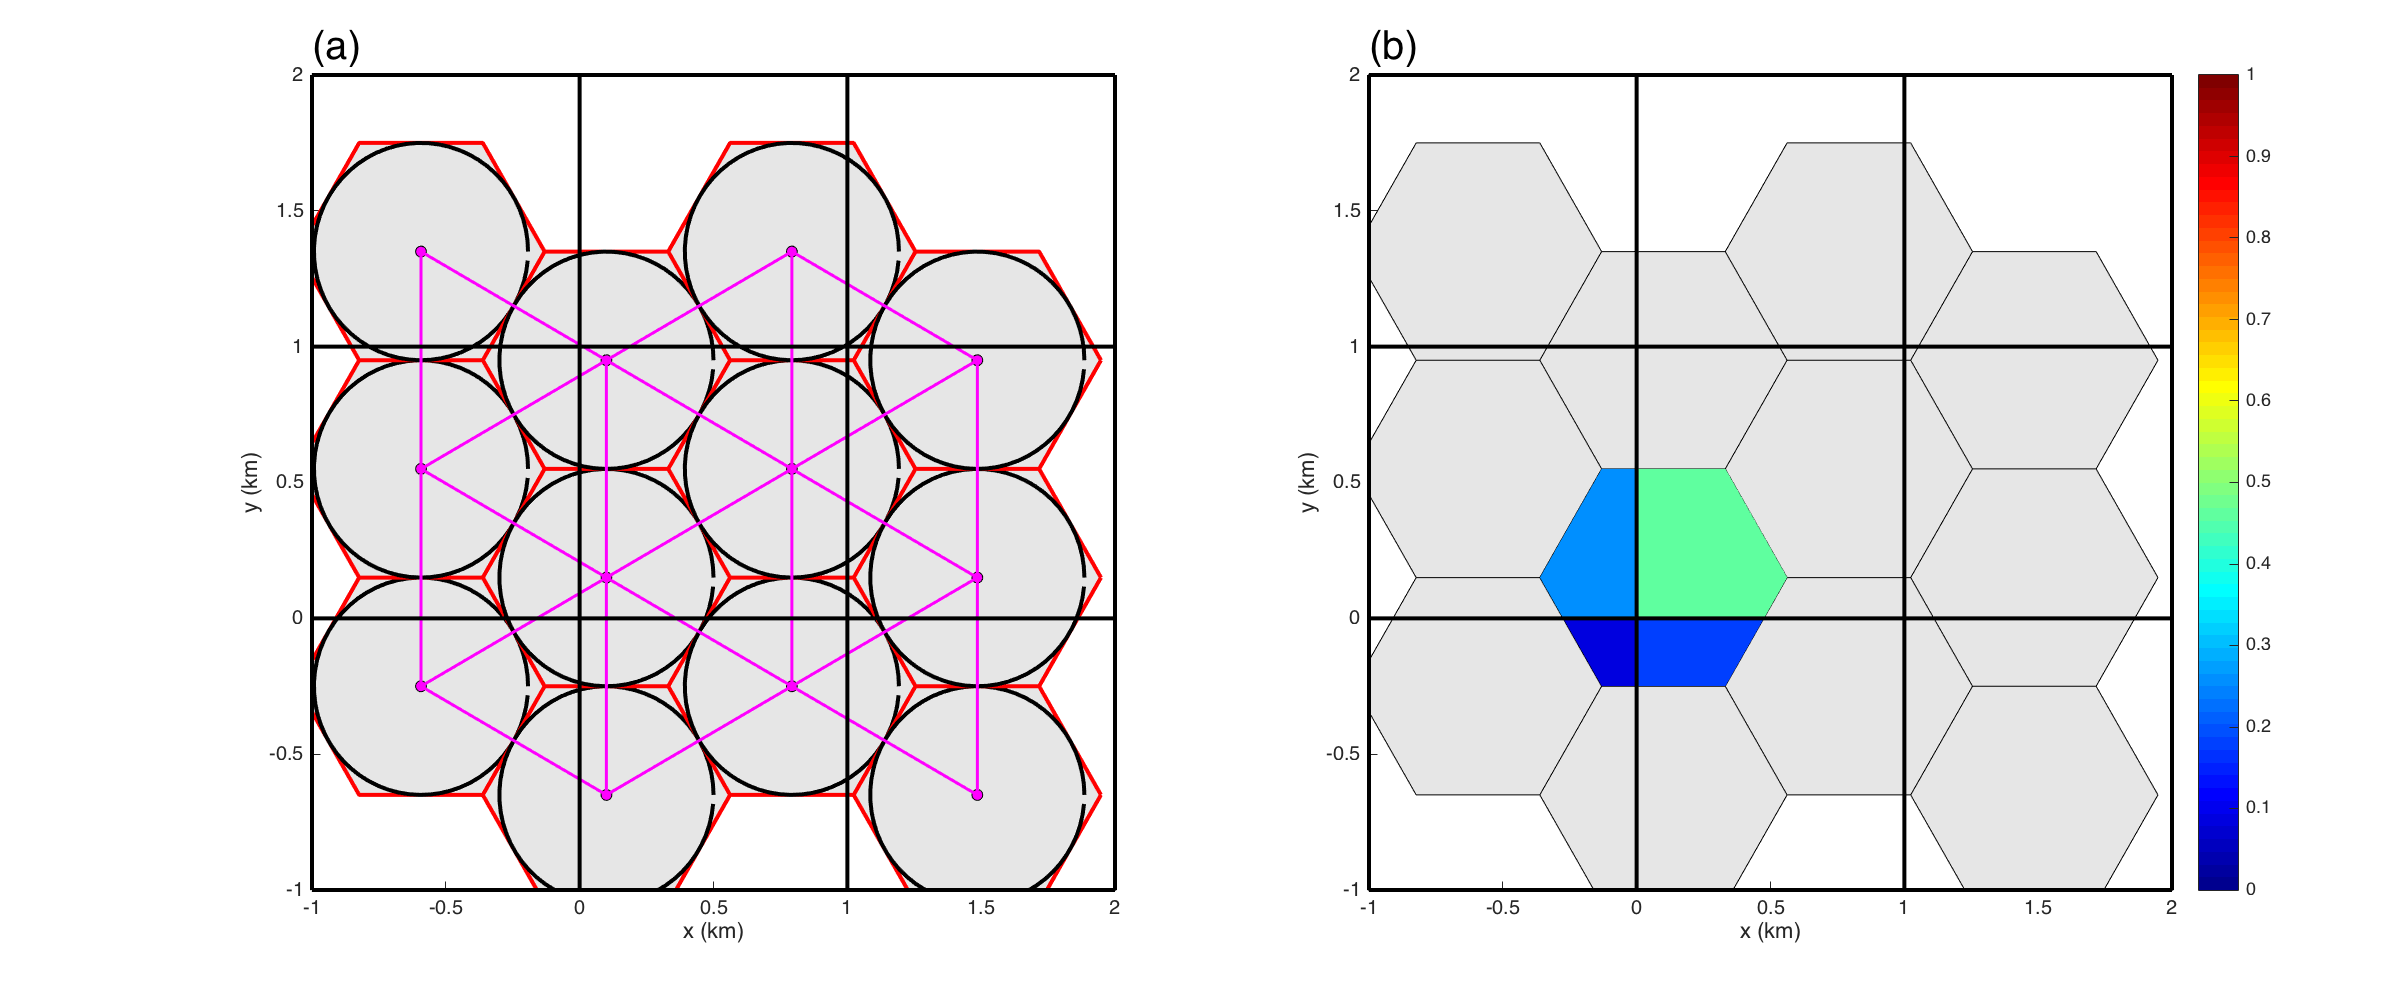
\includegraphics[width=0.99\textwidth]{/Users/alon/Desktop/files/Icebergs_clusters/Towards_Publication/Tech_paper/Github_stuff/Tech-paper/Figures/hexagon_intersection3.png}
%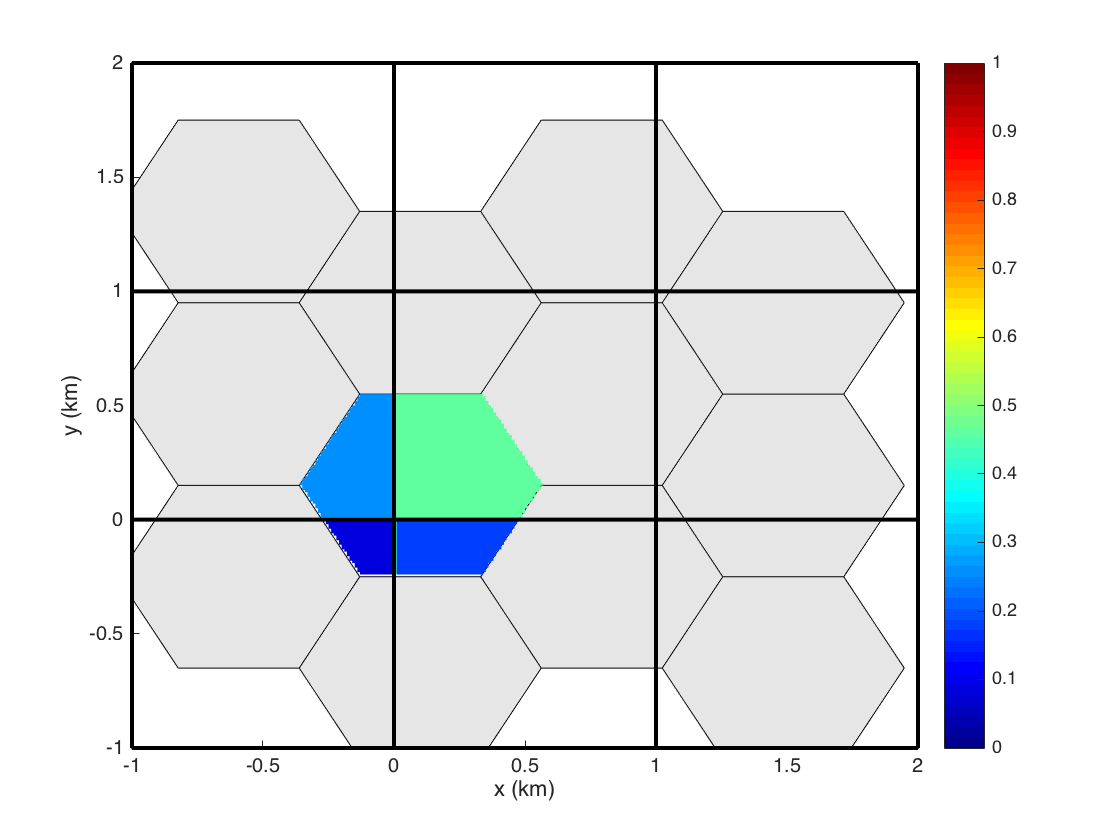
\includegraphics[width=0.69\textwidth]{/Users/alon/Desktop/files/Icebergs_clusters/Towards_Publication/Tech_paper/Github_stuff/Tech-paper/Figures/hex_on_a_grid}
\caption{ {(a) Ice element packing and geometry:  ice elements (purple dots) are initialized in a staggered lattice. For purposed of mass aggregation, the ice elements are assumed to have hexagonal shape (red hexagons). For purposed of element interactions, the ice elements are assumed to be circular (black circles). Elements are initially bonded to adjacent elements using numerical bonds (magenta lines). (b) Intersection of an hexagonal element and the ocean grid. The colors indicate the fraction of the hexagon that lies in each grid cell. These fractions are used as weights to spread the iceberg model properties to the ocean grid (see text for more details). }
\label{fig:Hex_intersections}}
\end{center}

\end{figure}
\clearpage



\begin{figure}
\begin{center}
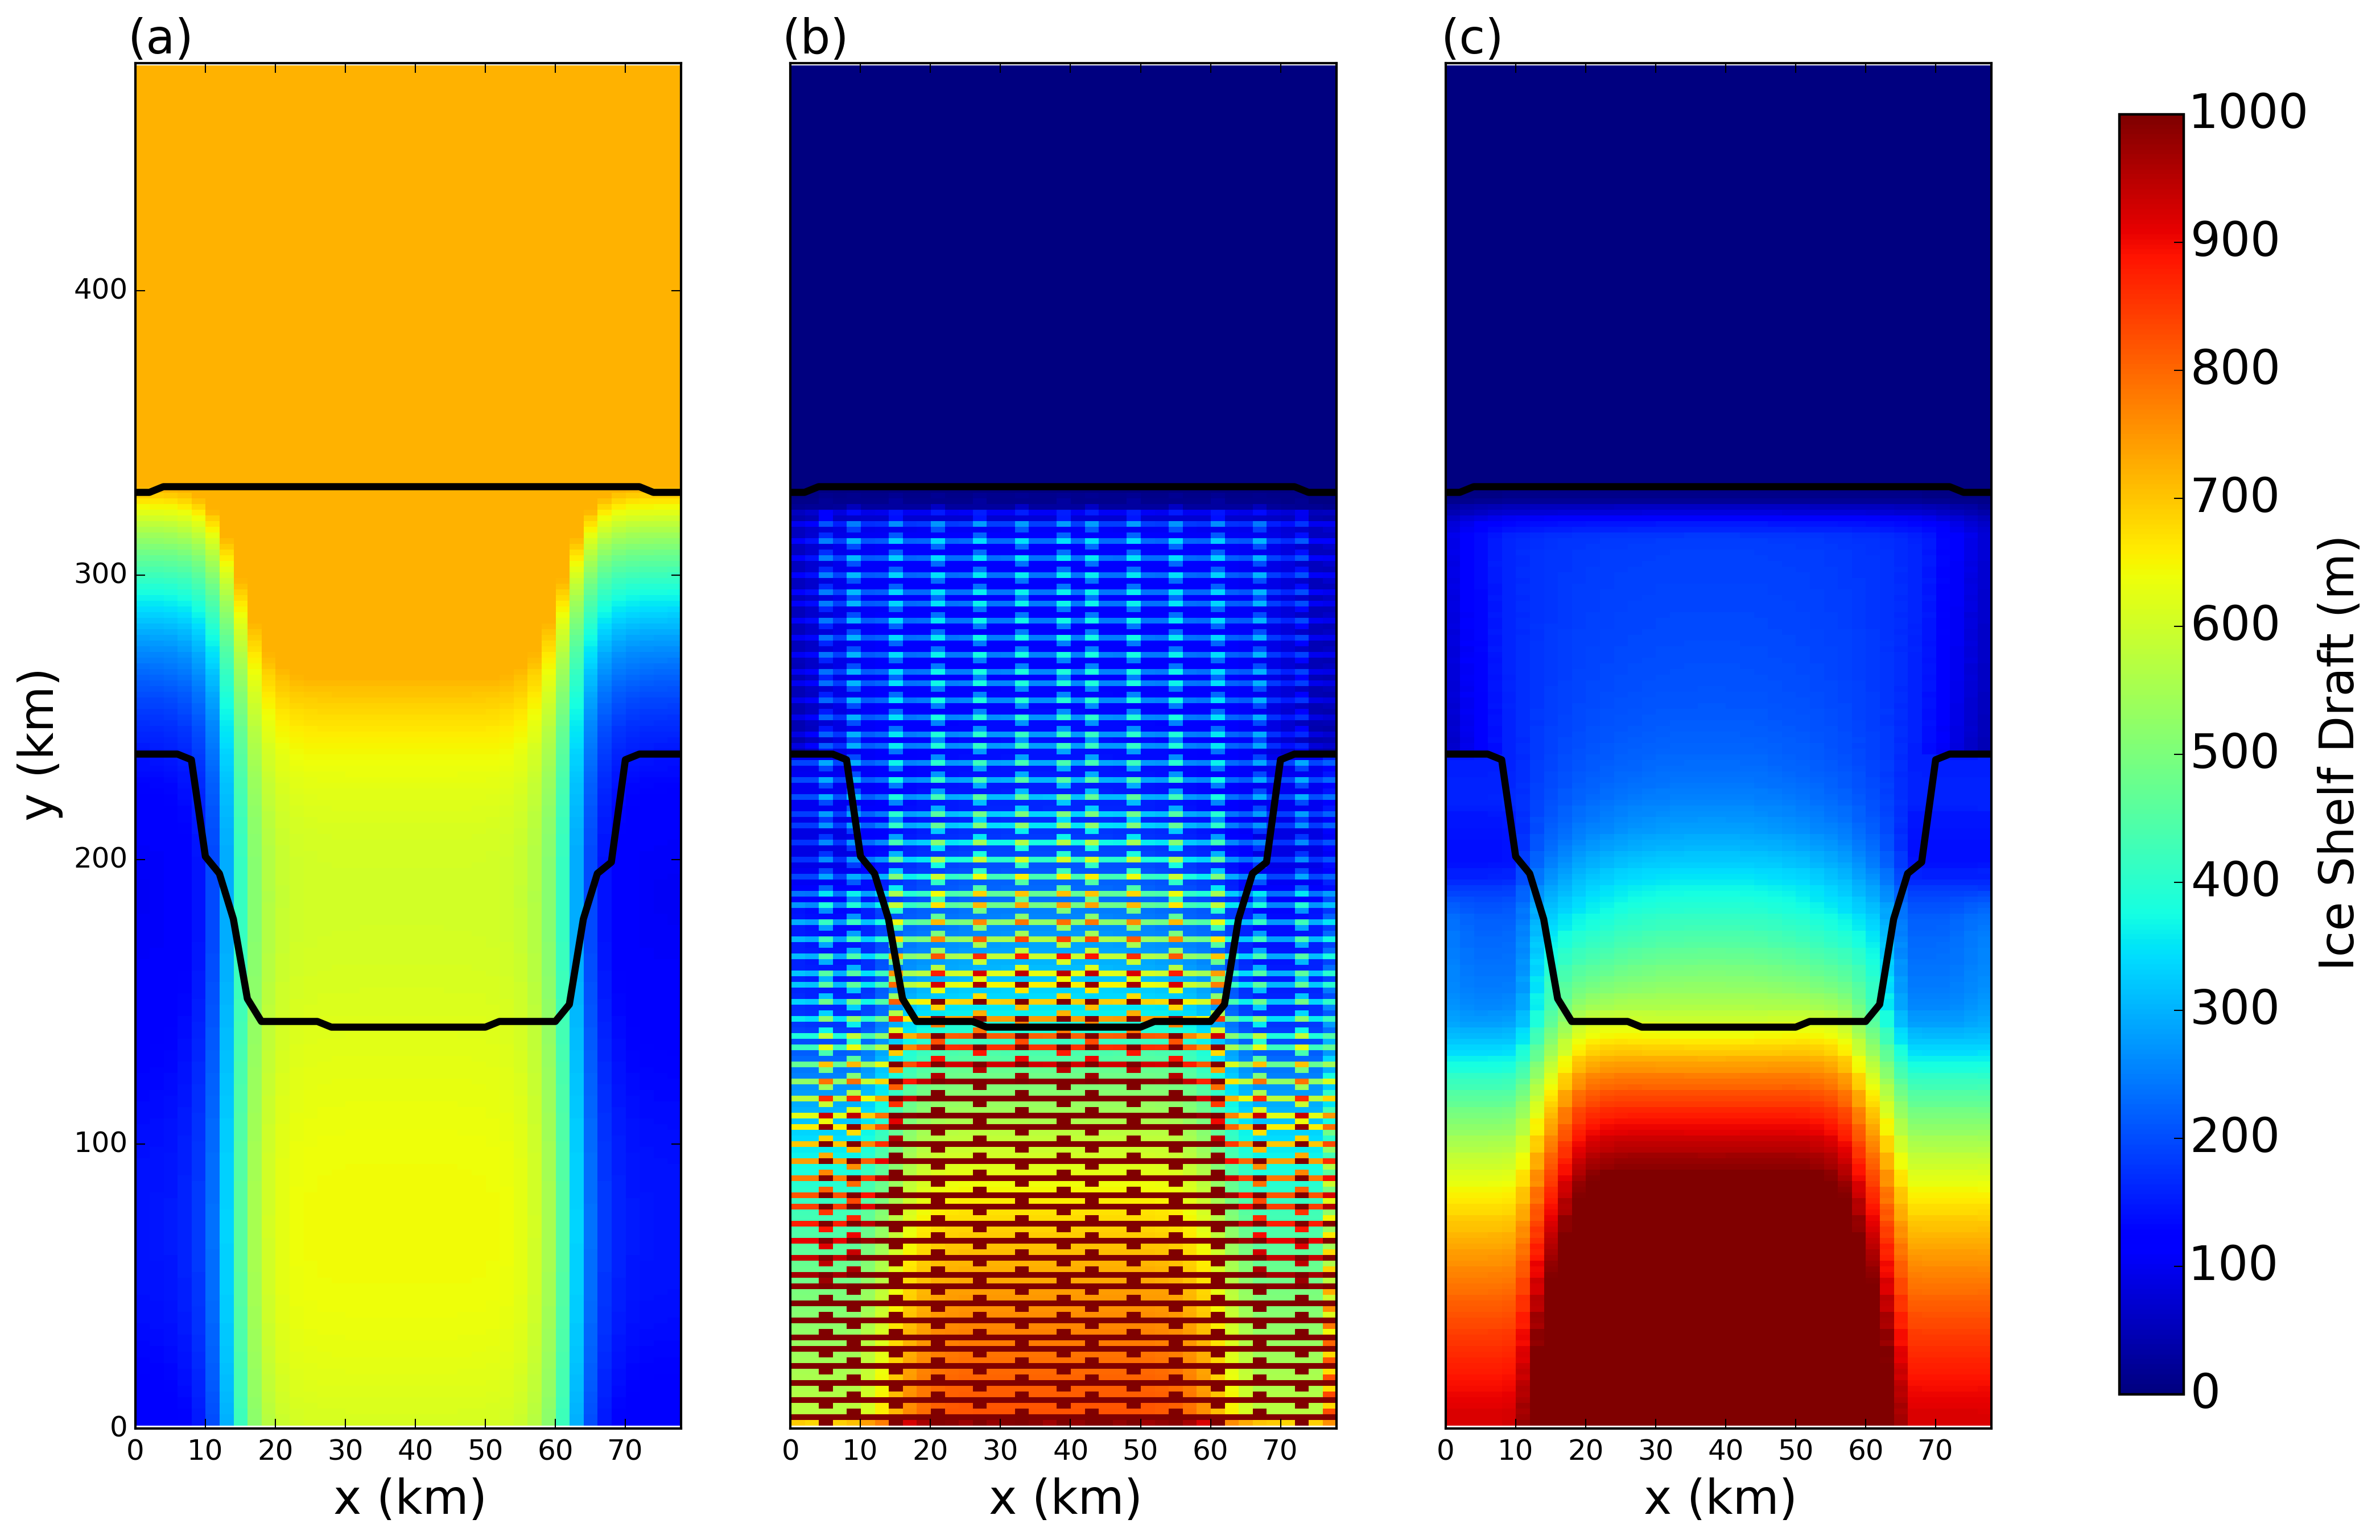
\includegraphics[width=0.99\textwidth]{/Users/alon/Desktop/files/Icebergs_clusters/Towards_Publication/Tech_paper/Github_stuff/Tech-paper/Figures/ALE_z_static_shelf_solo_D_mass_spread_mass.png}
\caption{ {(a) Ocean bottom topography and (c) ice-shelf draft used to initialized the tabular iceberg calving simulation. The ice draft is calculated from the total mass in an ocean grid cell after the mass-spreading interpolation has been applied (as explained in Section 2.3). Panel (b) shows the initial ice draft that would be calculated if the mass-spreading interpolation were not used (i.e. elements treated as point masses).} \label{fig:ISOMIP_mass_and_topog}}
\end{center}
\end{figure}
 \clearpage
 
 

 

\begin{figure}
\begin{center}
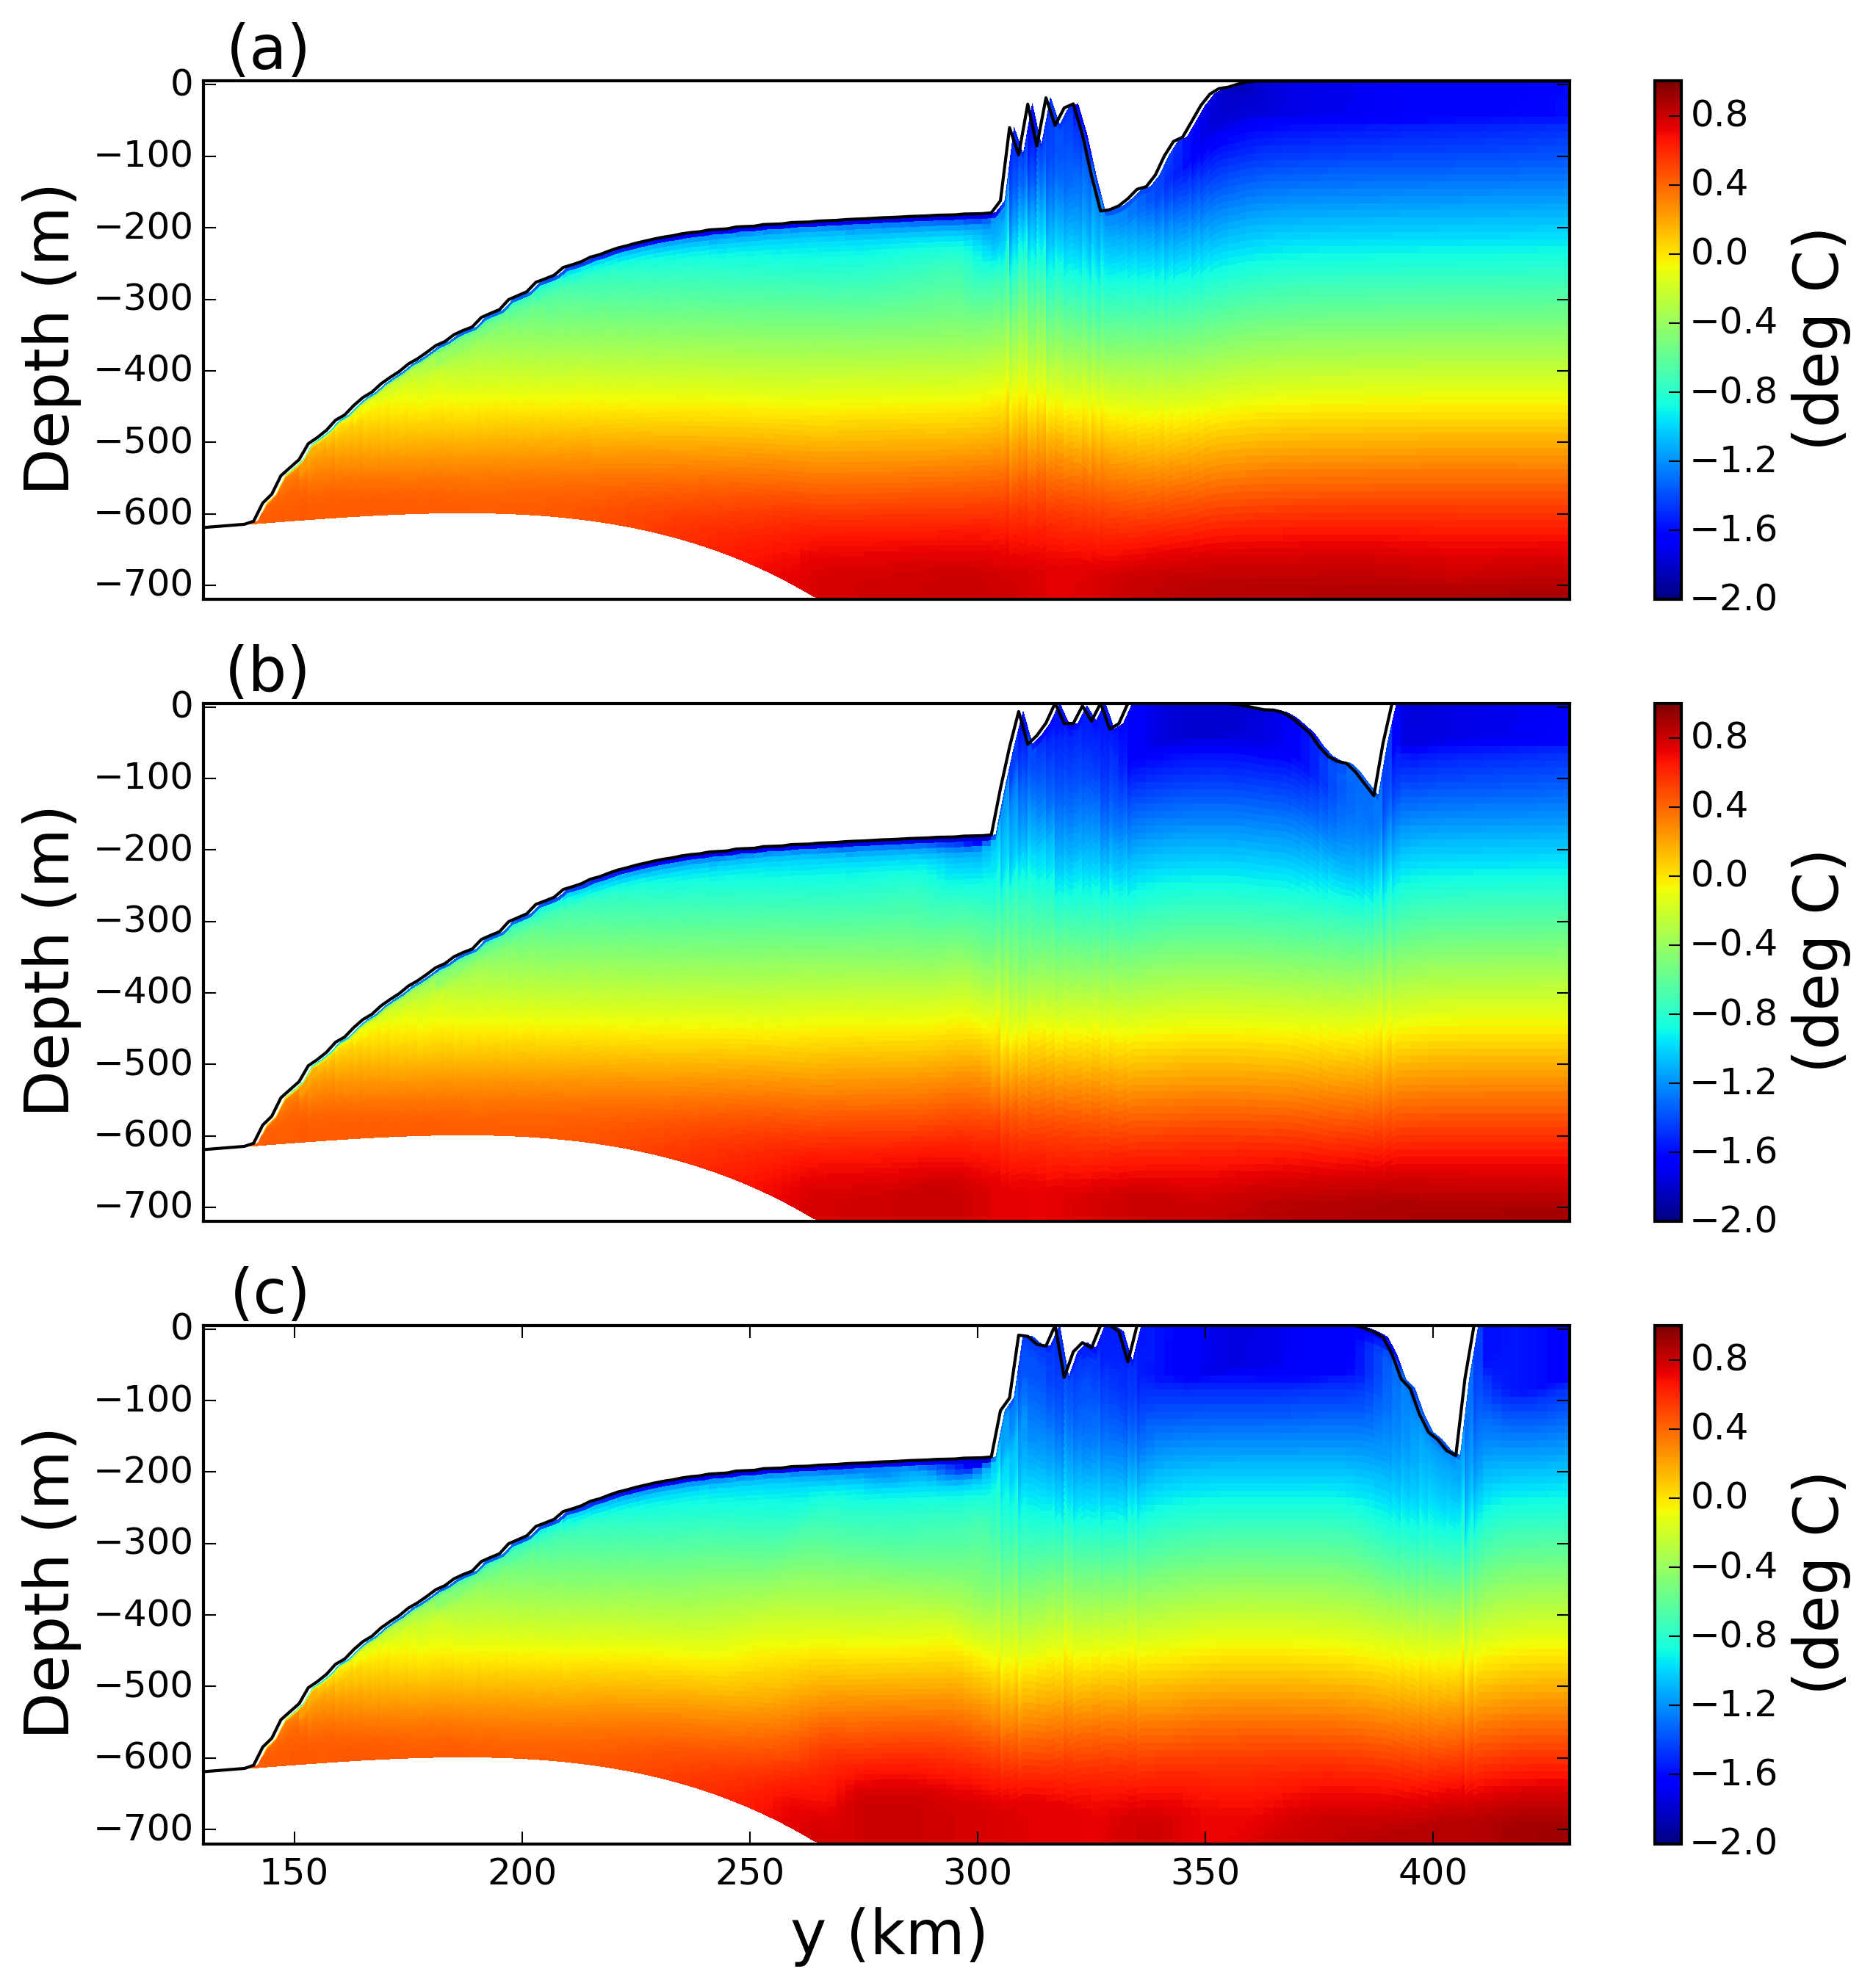
\includegraphics[width=0.99\textwidth]{/Users/alon/Desktop/files/Icebergs_clusters/Towards_Publication/Tech_paper/Github_stuff/Tech-paper/Figures/snapshots_ALE_z_Mixed_Melt_Collapse_temp_layers_x12.png}
\caption{ {Snapshots of vertical sections of ocean temperature at $x$=54~km in the tabular-iceberg-calving Control experiment. Snapshots are taken (a) 7, (b) 15, and (c) 30 days after calving. The position of the vertical transects is shown by the dashed lines in Figure \ref{fig:SST_Collapse}c.}
\label{fig:Temperature_section_Collapse}}
\end{center}
\end{figure}
 \clearpage
 




\begin{figure}
\begin{center}
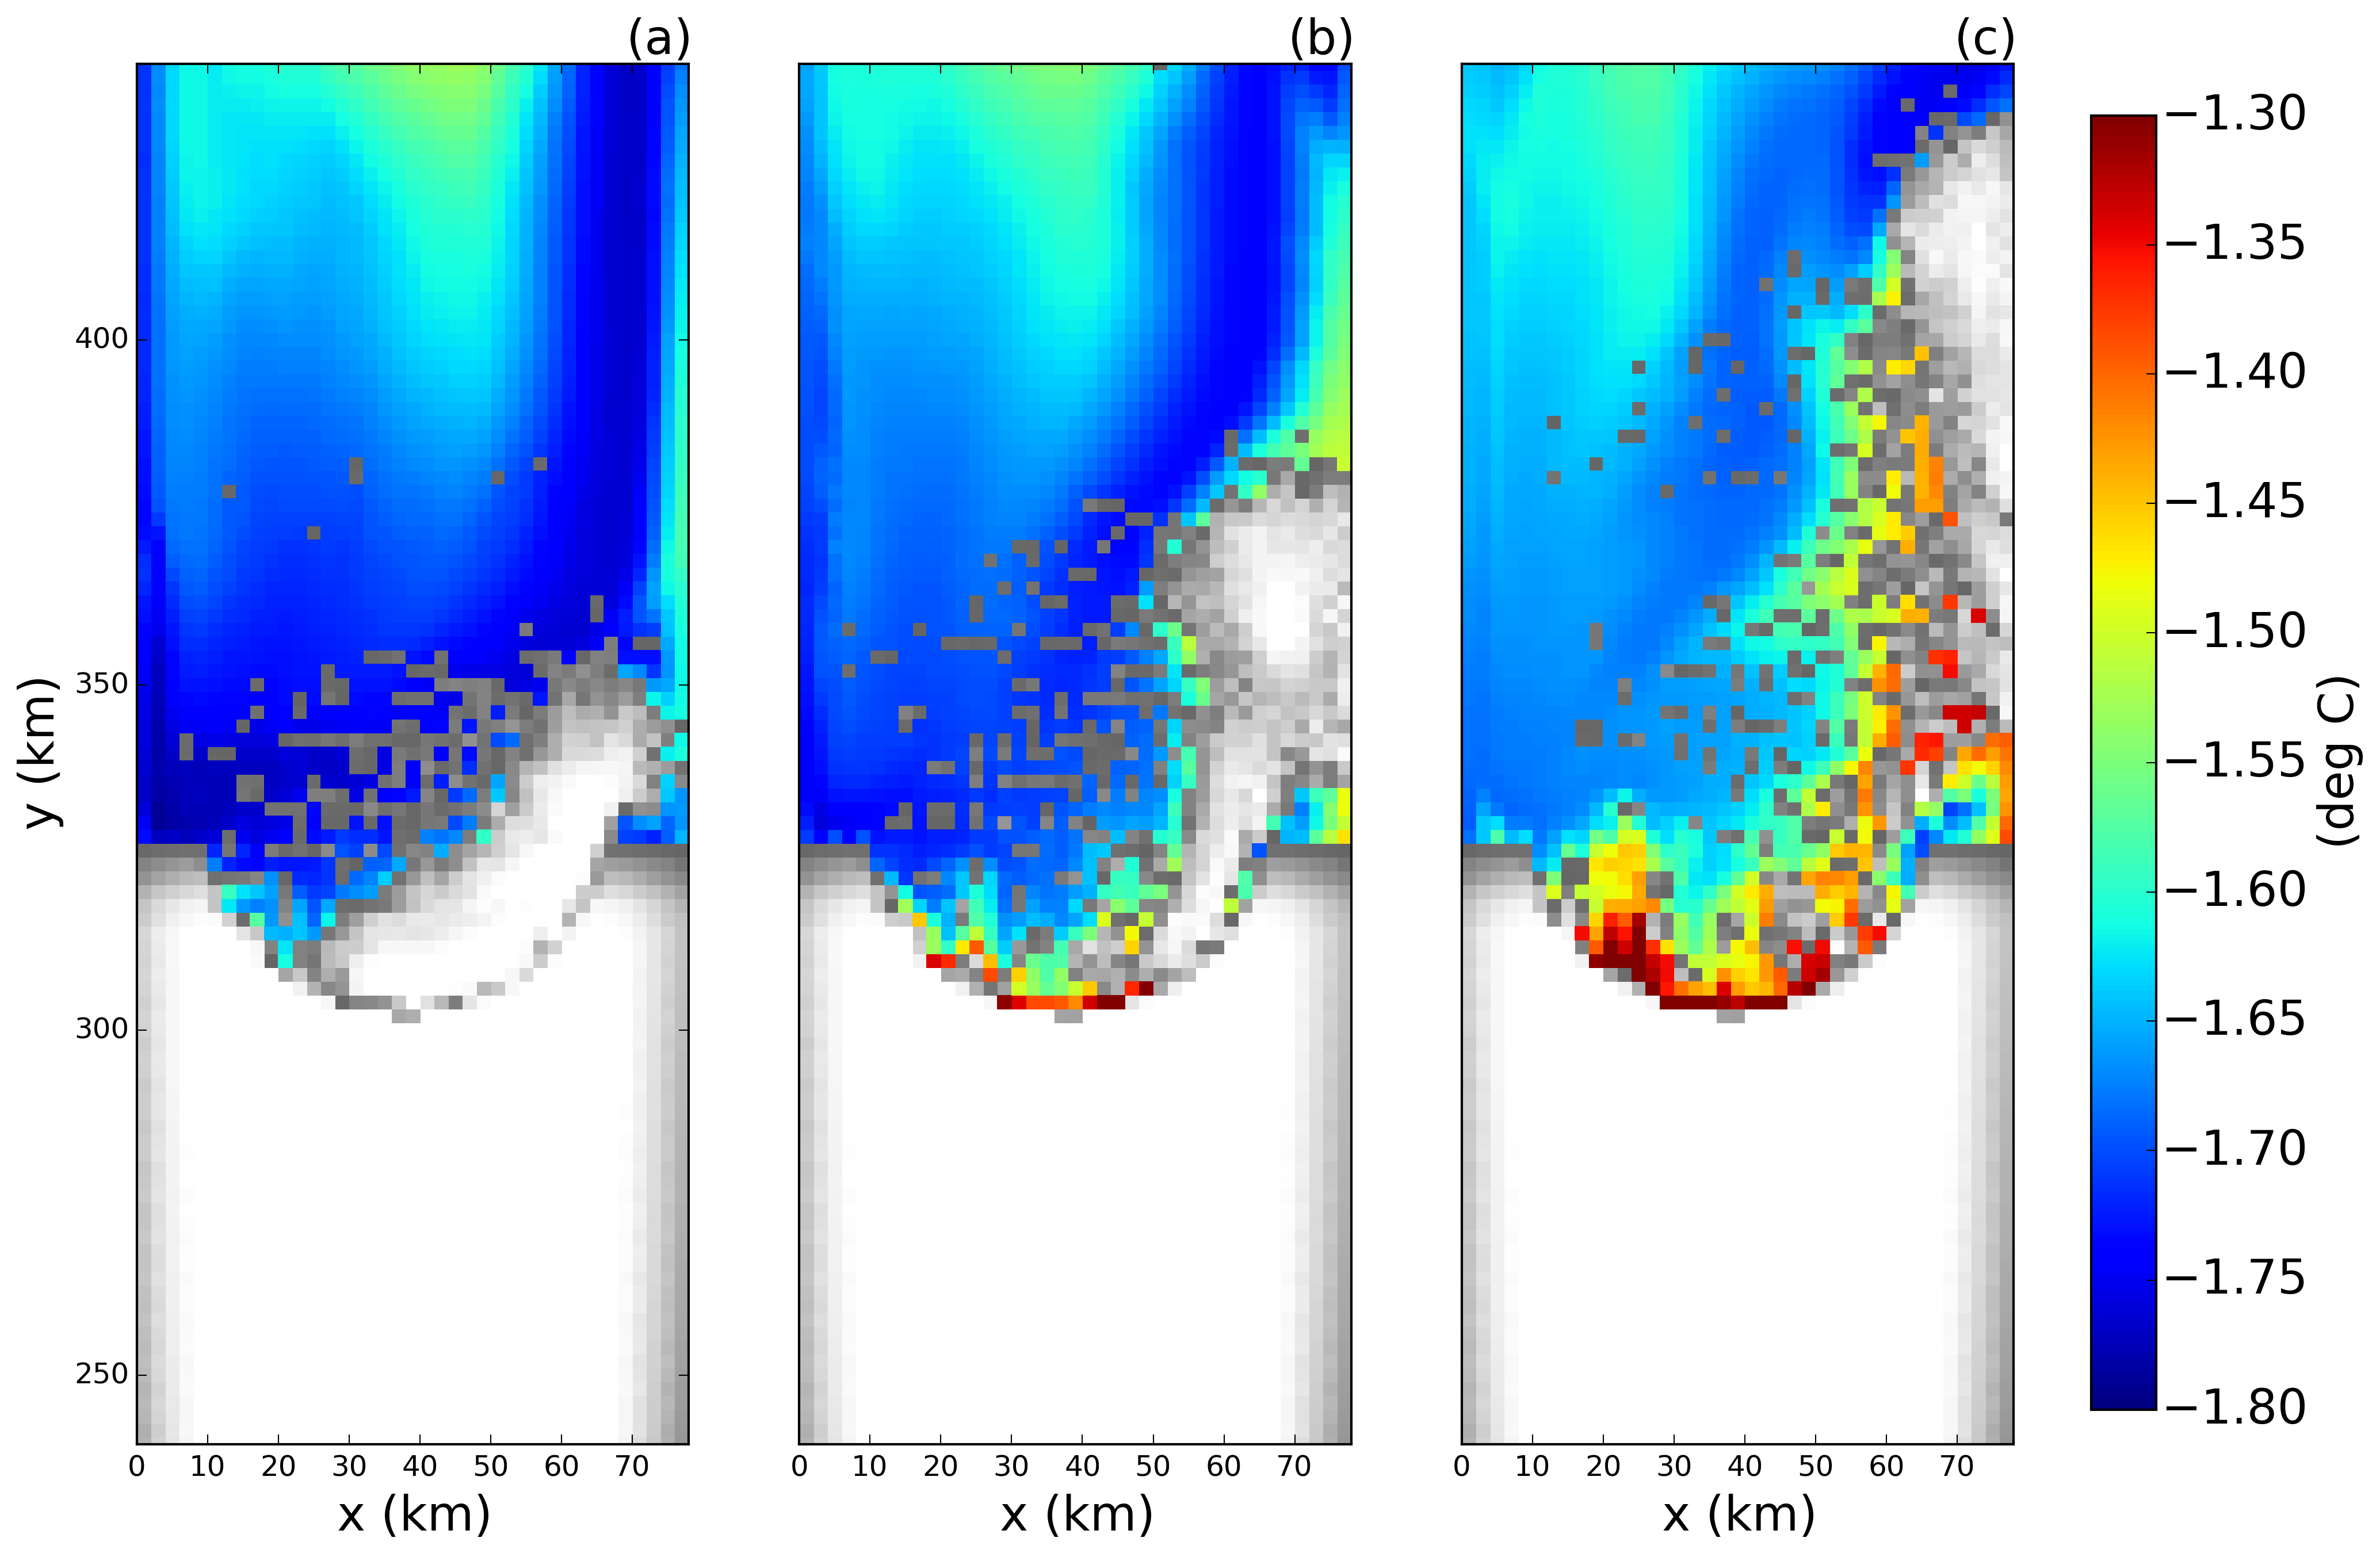
\includegraphics[width=0.99\textwidth]{/Users/alon/Desktop/files/Icebergs_clusters/Towards_Publication/Tech_paper/Github_stuff/Tech-paper/Figures/snapshots_ALE_z_Drift_temp.png}
\caption{ {No bonds simulation: Snapshots of the sea surface temperature for a simulation where all bonds have been broken. Snapshots are taken (a) 7, (b) 15, and (c) 30 days after calving. Grid cells with ice mass > $10^{4}$ kg are plotted in white, with grey shading indicating thinner ice.}
\label{fig:Drift_berg}}
\end{center}
\end{figure}
 \clearpage



\begin{figure}
\begin{center}
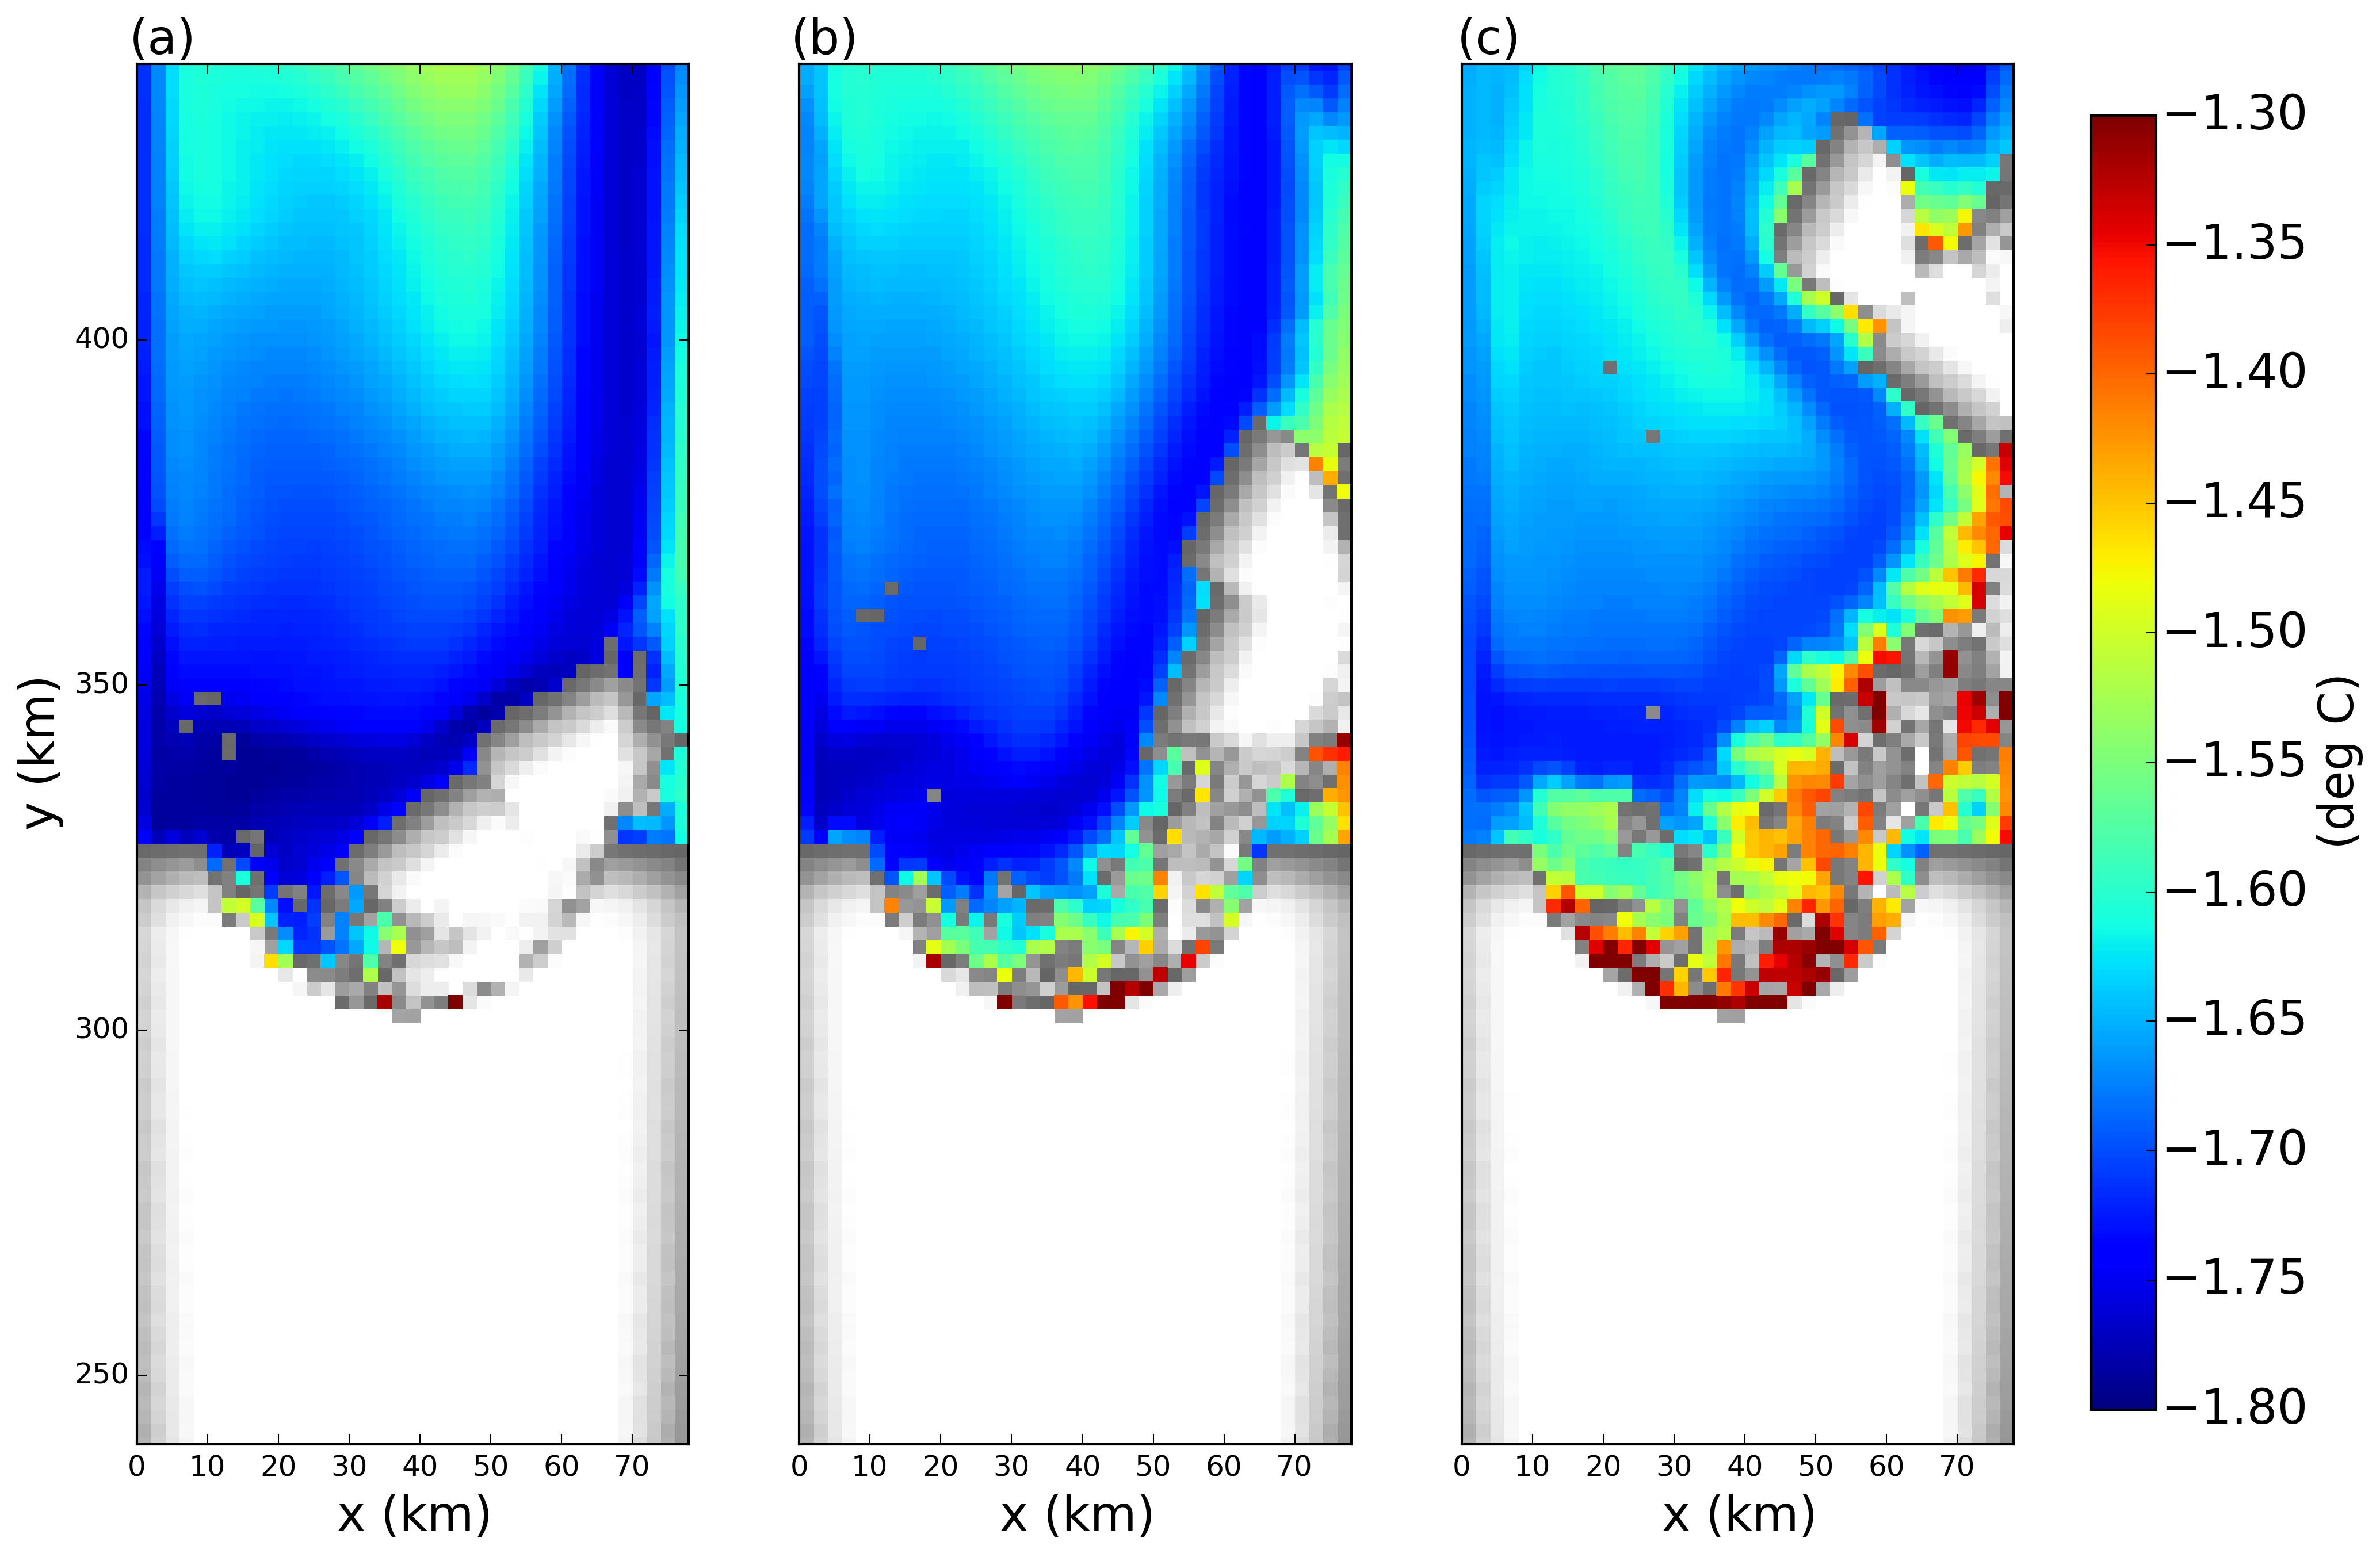
\includegraphics[width=0.99\textwidth]{/Users/alon/Desktop/files/Icebergs_clusters/Towards_Publication/Tech_paper/Github_stuff/Tech-paper/Figures/snapshots_ALE_z_Splitting_temp.png}
\caption{ {Iceberg splitting simulation: Snapshots of the sea surface temperature for the iceberg splitting simulation. Snapshots are taken (a) 7, (b) 15, and (c) 30 days after calving. Grid cells with ice mass > $10^{4}$ kg are plotted in white, with grey shading indicating thinner ice.}
\label{fig:Splitting_berg}}
\end{center}
\end{figure}
 \clearpage





\begin{figure}
\begin{center}
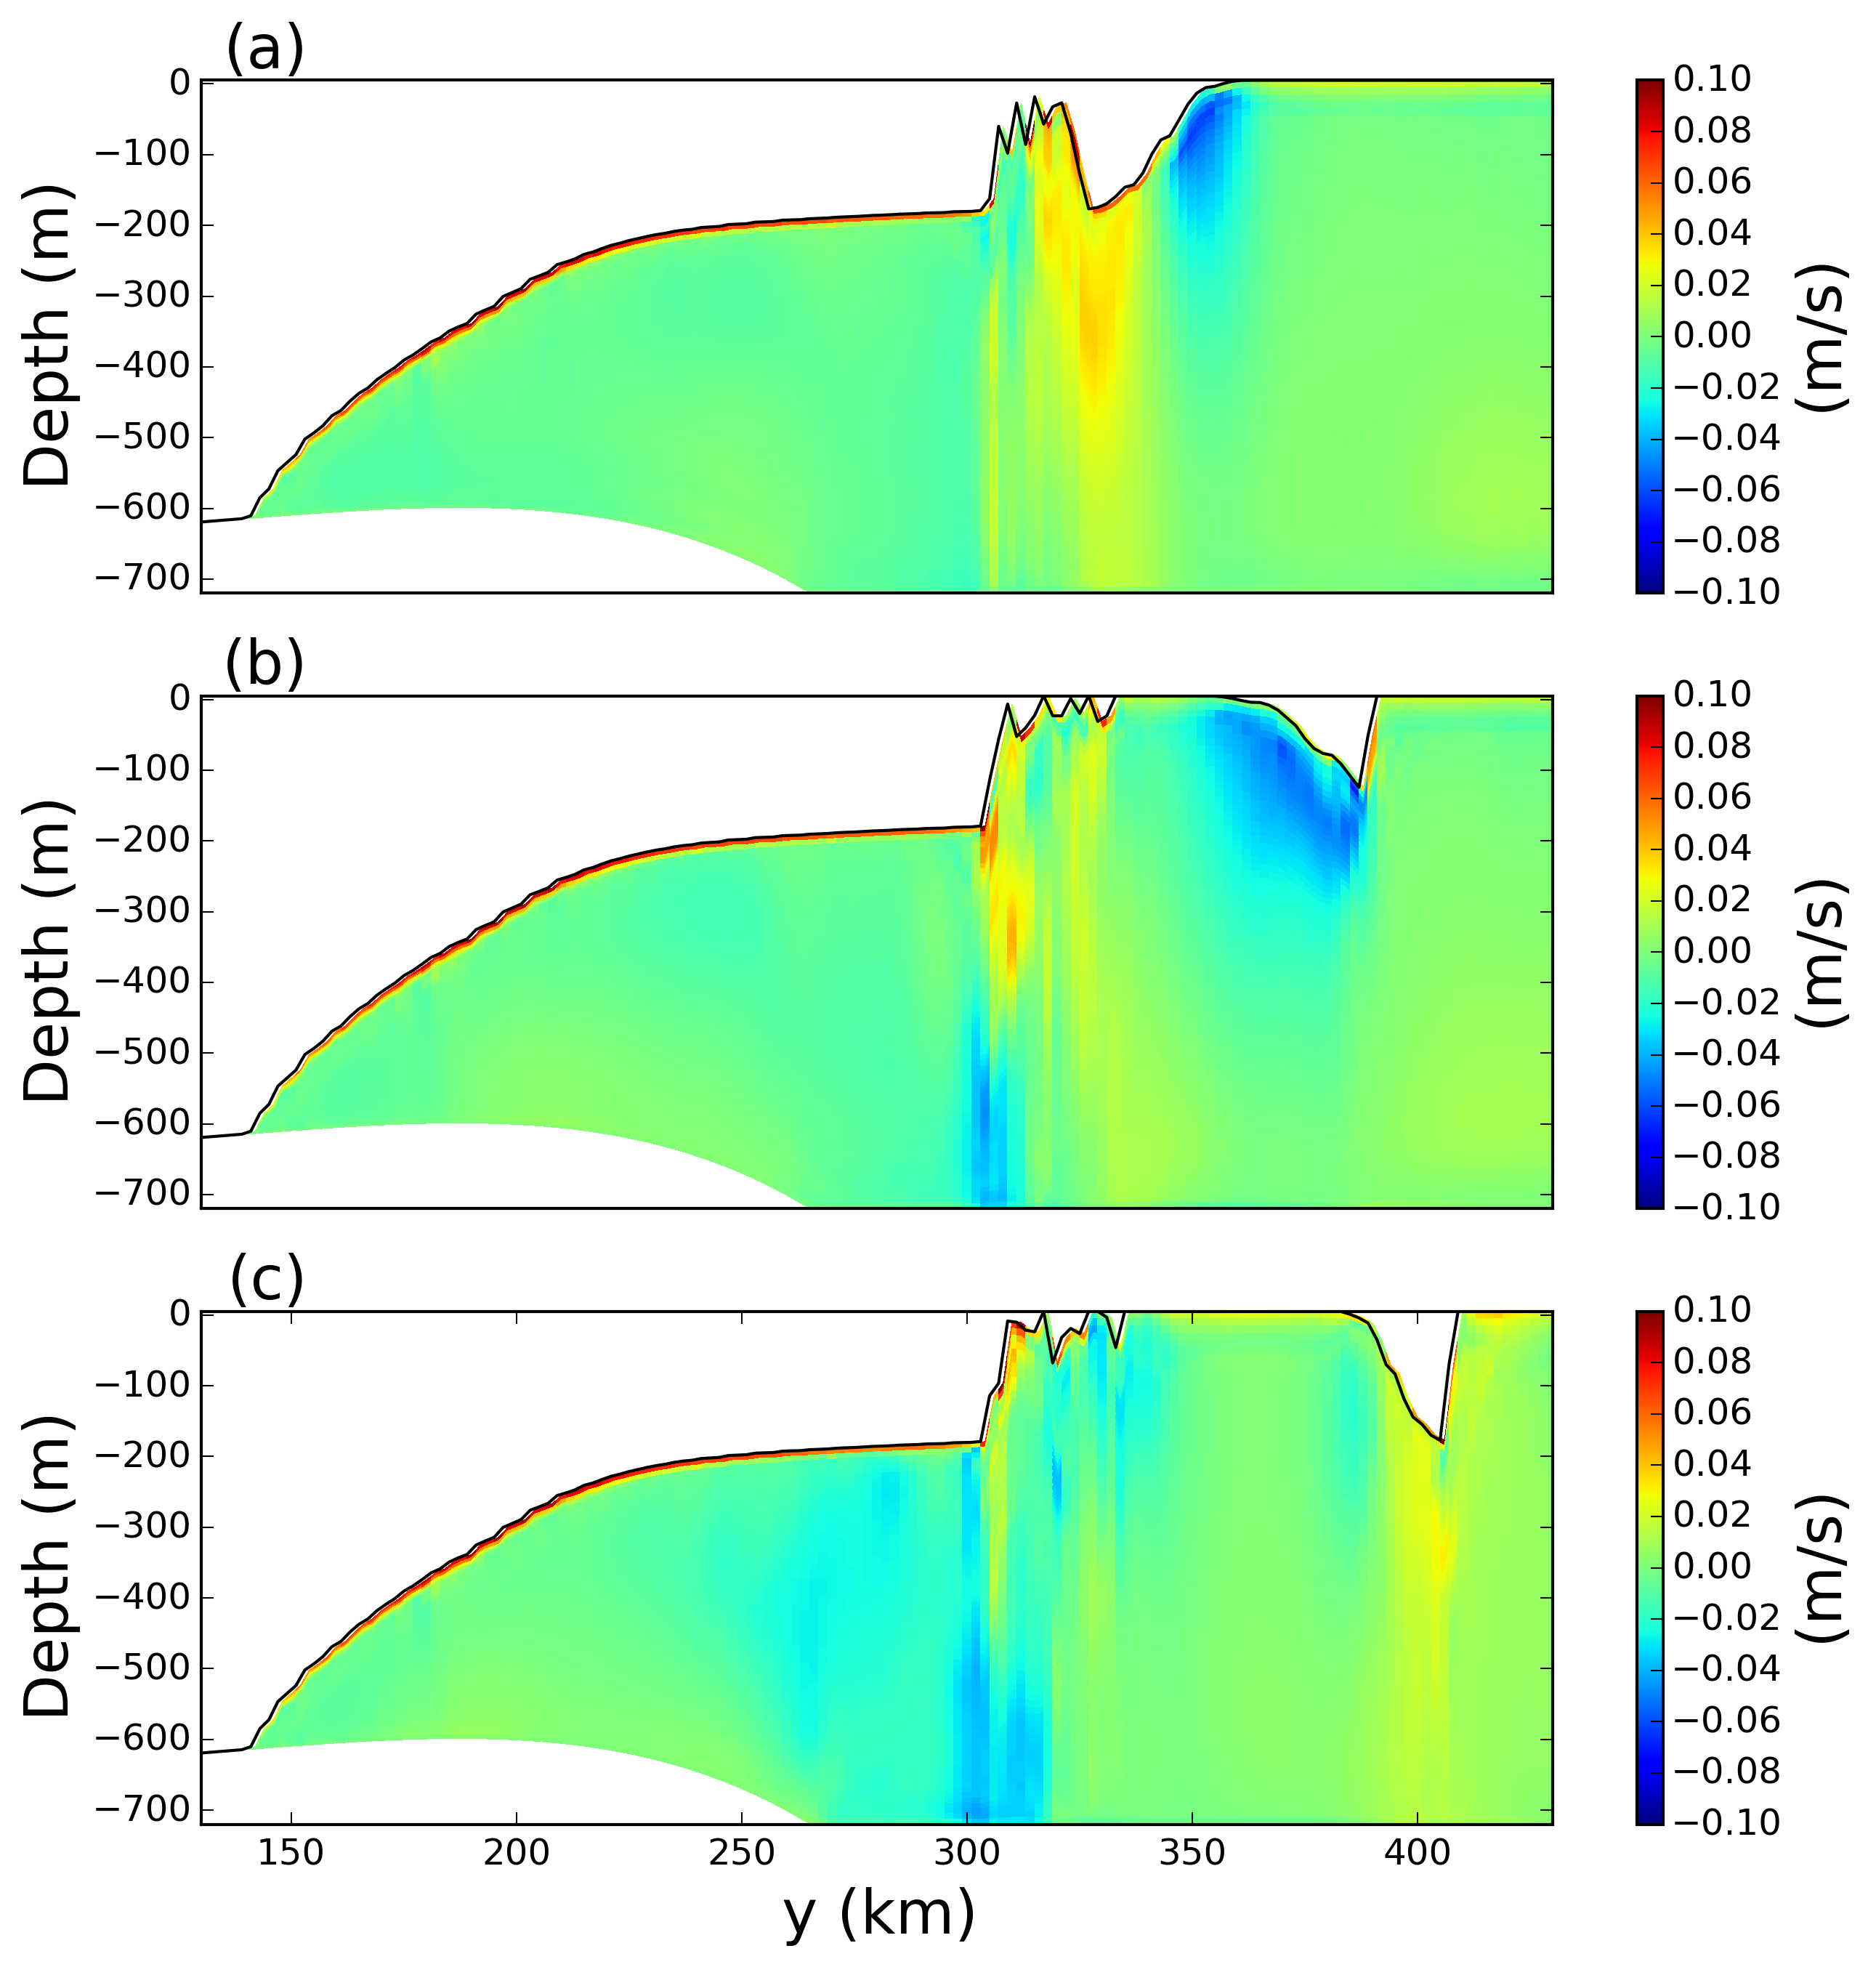
\includegraphics[width=0.99\textwidth]{/Users/alon/Desktop/files/Icebergs_clusters/Towards_Publication/Tech_paper/Github_stuff/Tech-paper/Figures/snapshots_ALE_z_Mixed_Melt_Collapse_v_layers_x12.png}
\caption{ {Snapshots of vertical sections of meridional velocity at $x$=54~km in the tabular-iceberg-calving Control experiment. Snapshots are taken (a) 7, (b) 15, and (c) 30 days after calving. The position of the transects is shown by the dashed line in Figure \ref{fig:SST_Collapse}c.}
\label{fig:Velocity_section_Collapse}}
\end{center}
\end{figure}
 \clearpage




\begin{figure}
\begin{center}
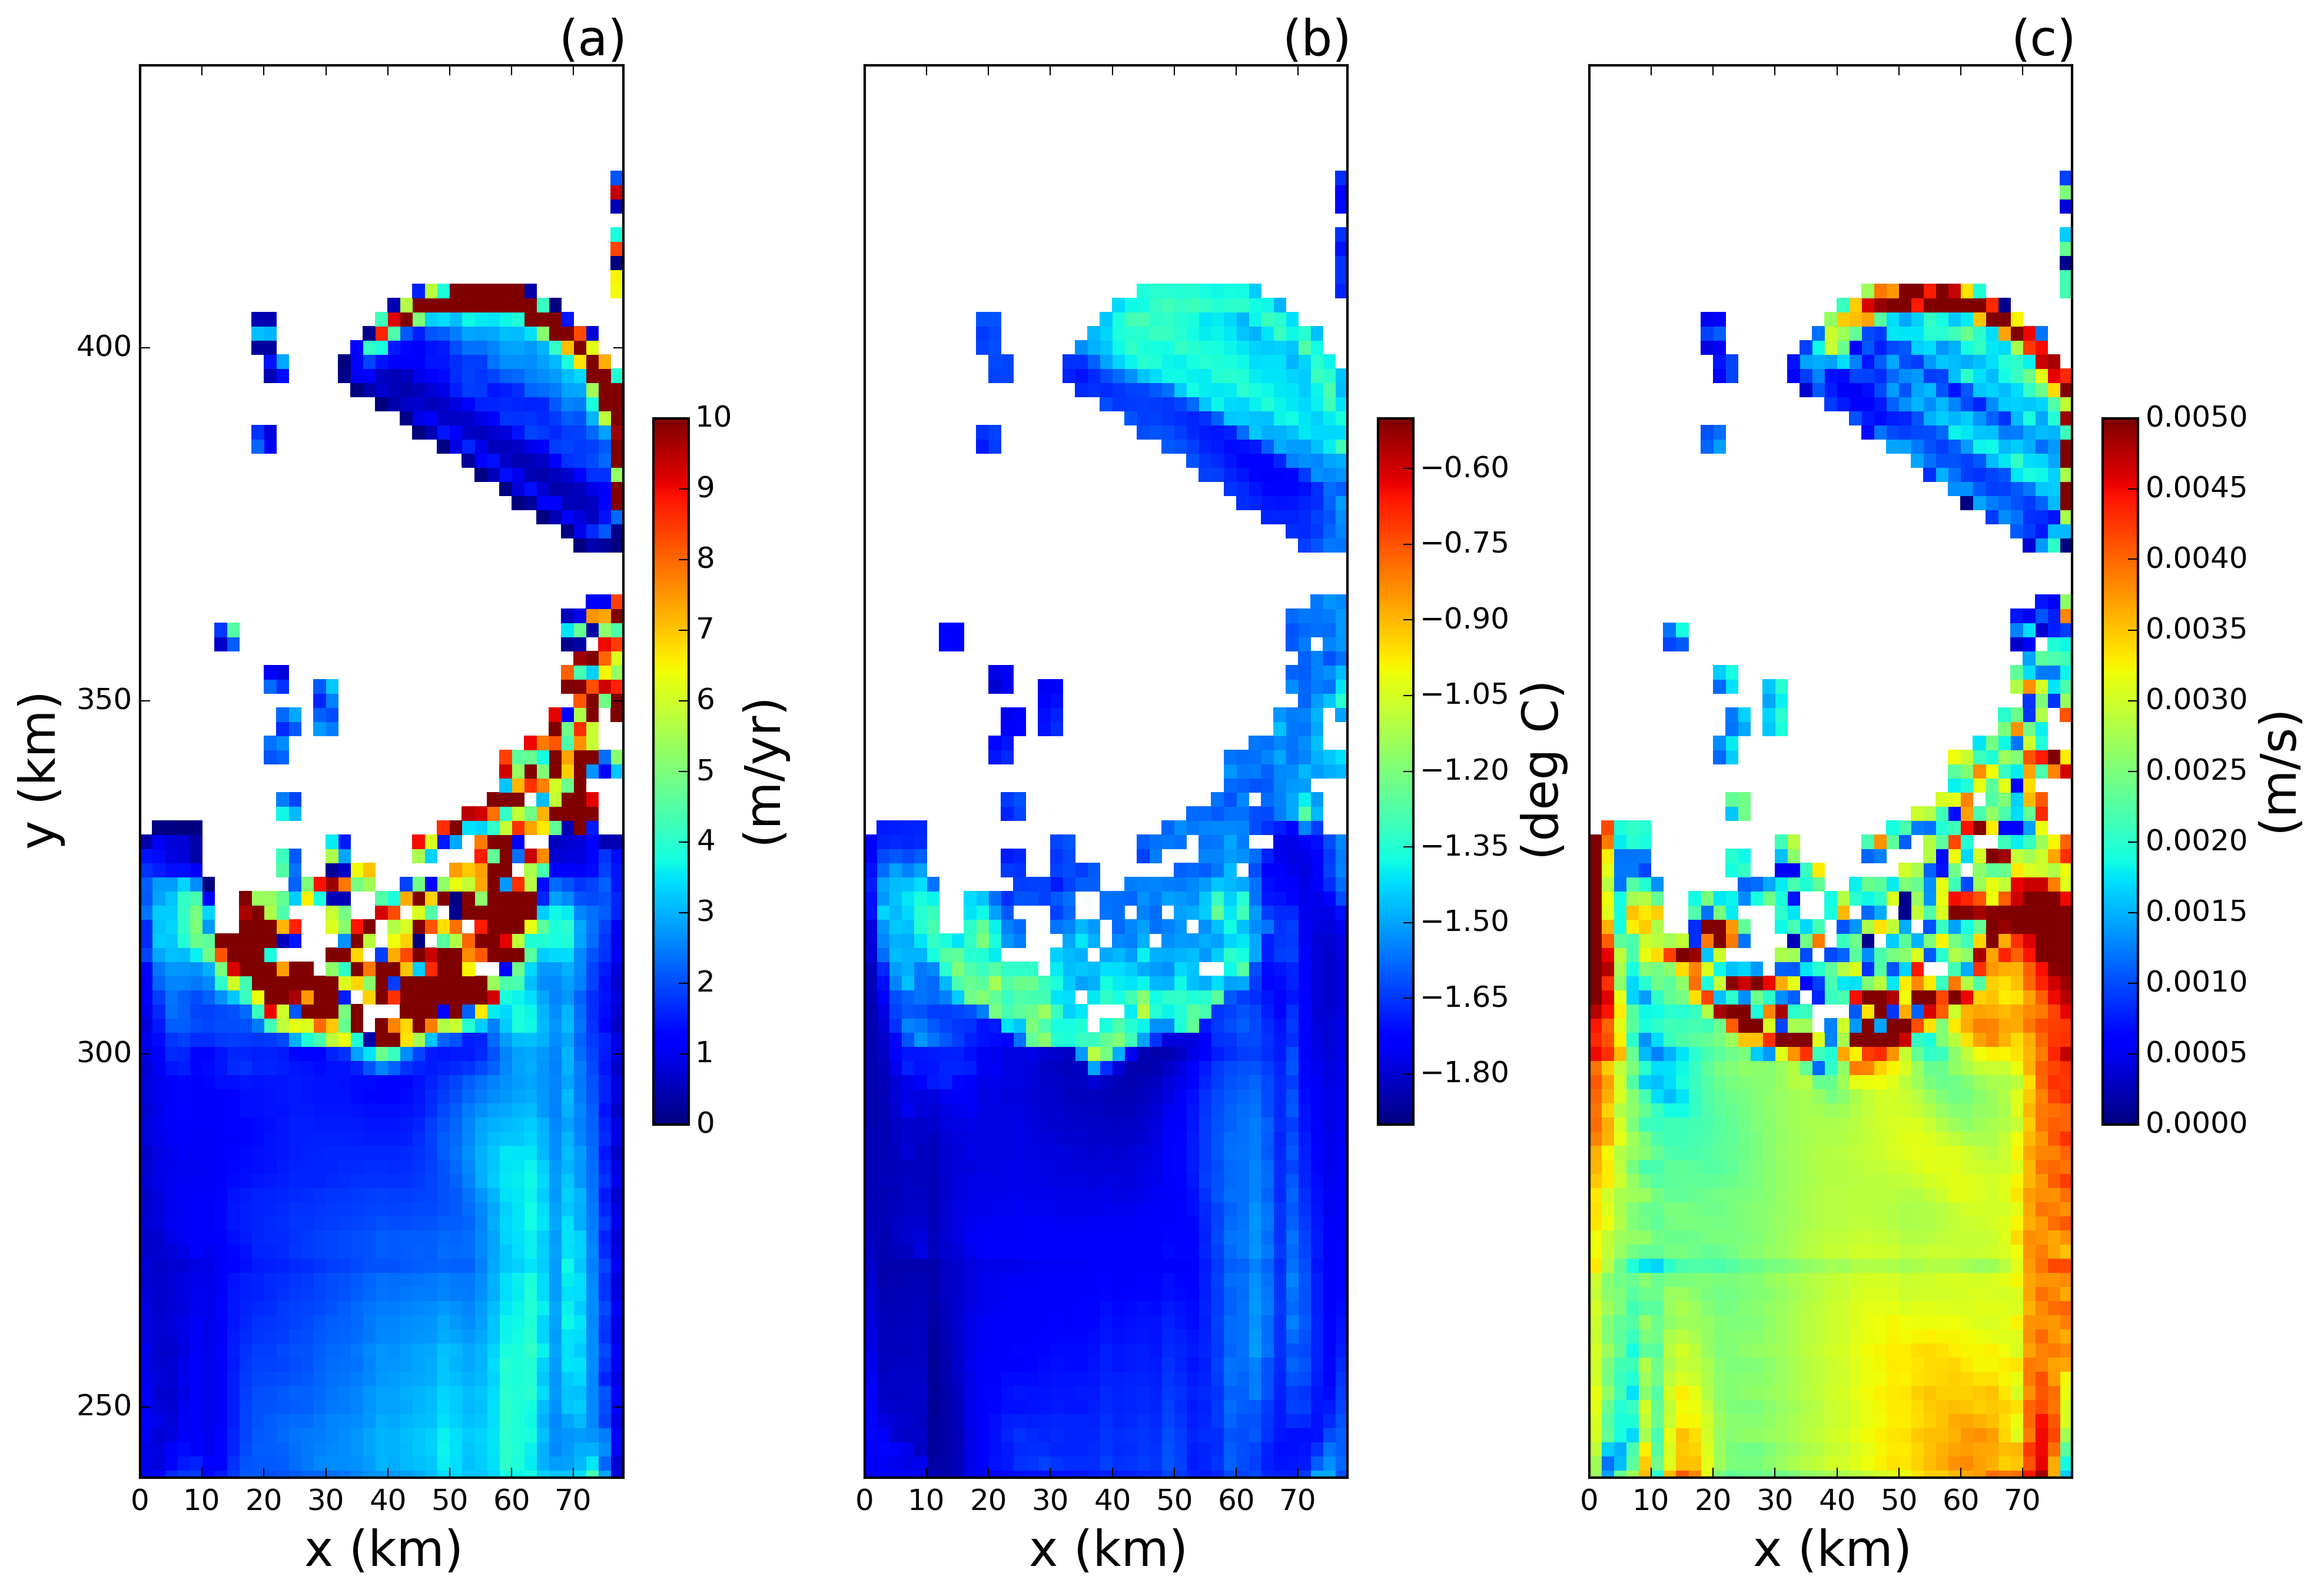
\includegraphics[width=0.99\textwidth]{/Users/alon/Desktop/files/Icebergs_clusters/Towards_Publication/Tech_paper/Github_stuff/Tech-paper/Figures/ALE_z_static_shelf_solo_melt_m_per_year_sst_ustar_iceberg_calved.png}
\caption{ {Results of the tabular-iceberg-calving experiment 30 days after the iceberg calves. The three panels show snapshots of the (a) melt rate, (b) top-of-ocean temperature and (c) the frictional velocity, $u^{*}$, at the base of the ice shelf. Ocean grid cells without ice are masked out in grey.}
\label{fig:Collapse_solo_melt}}
\end{center}
\end{figure}
 \clearpage








%\begin{figure}
%\begin{center}
%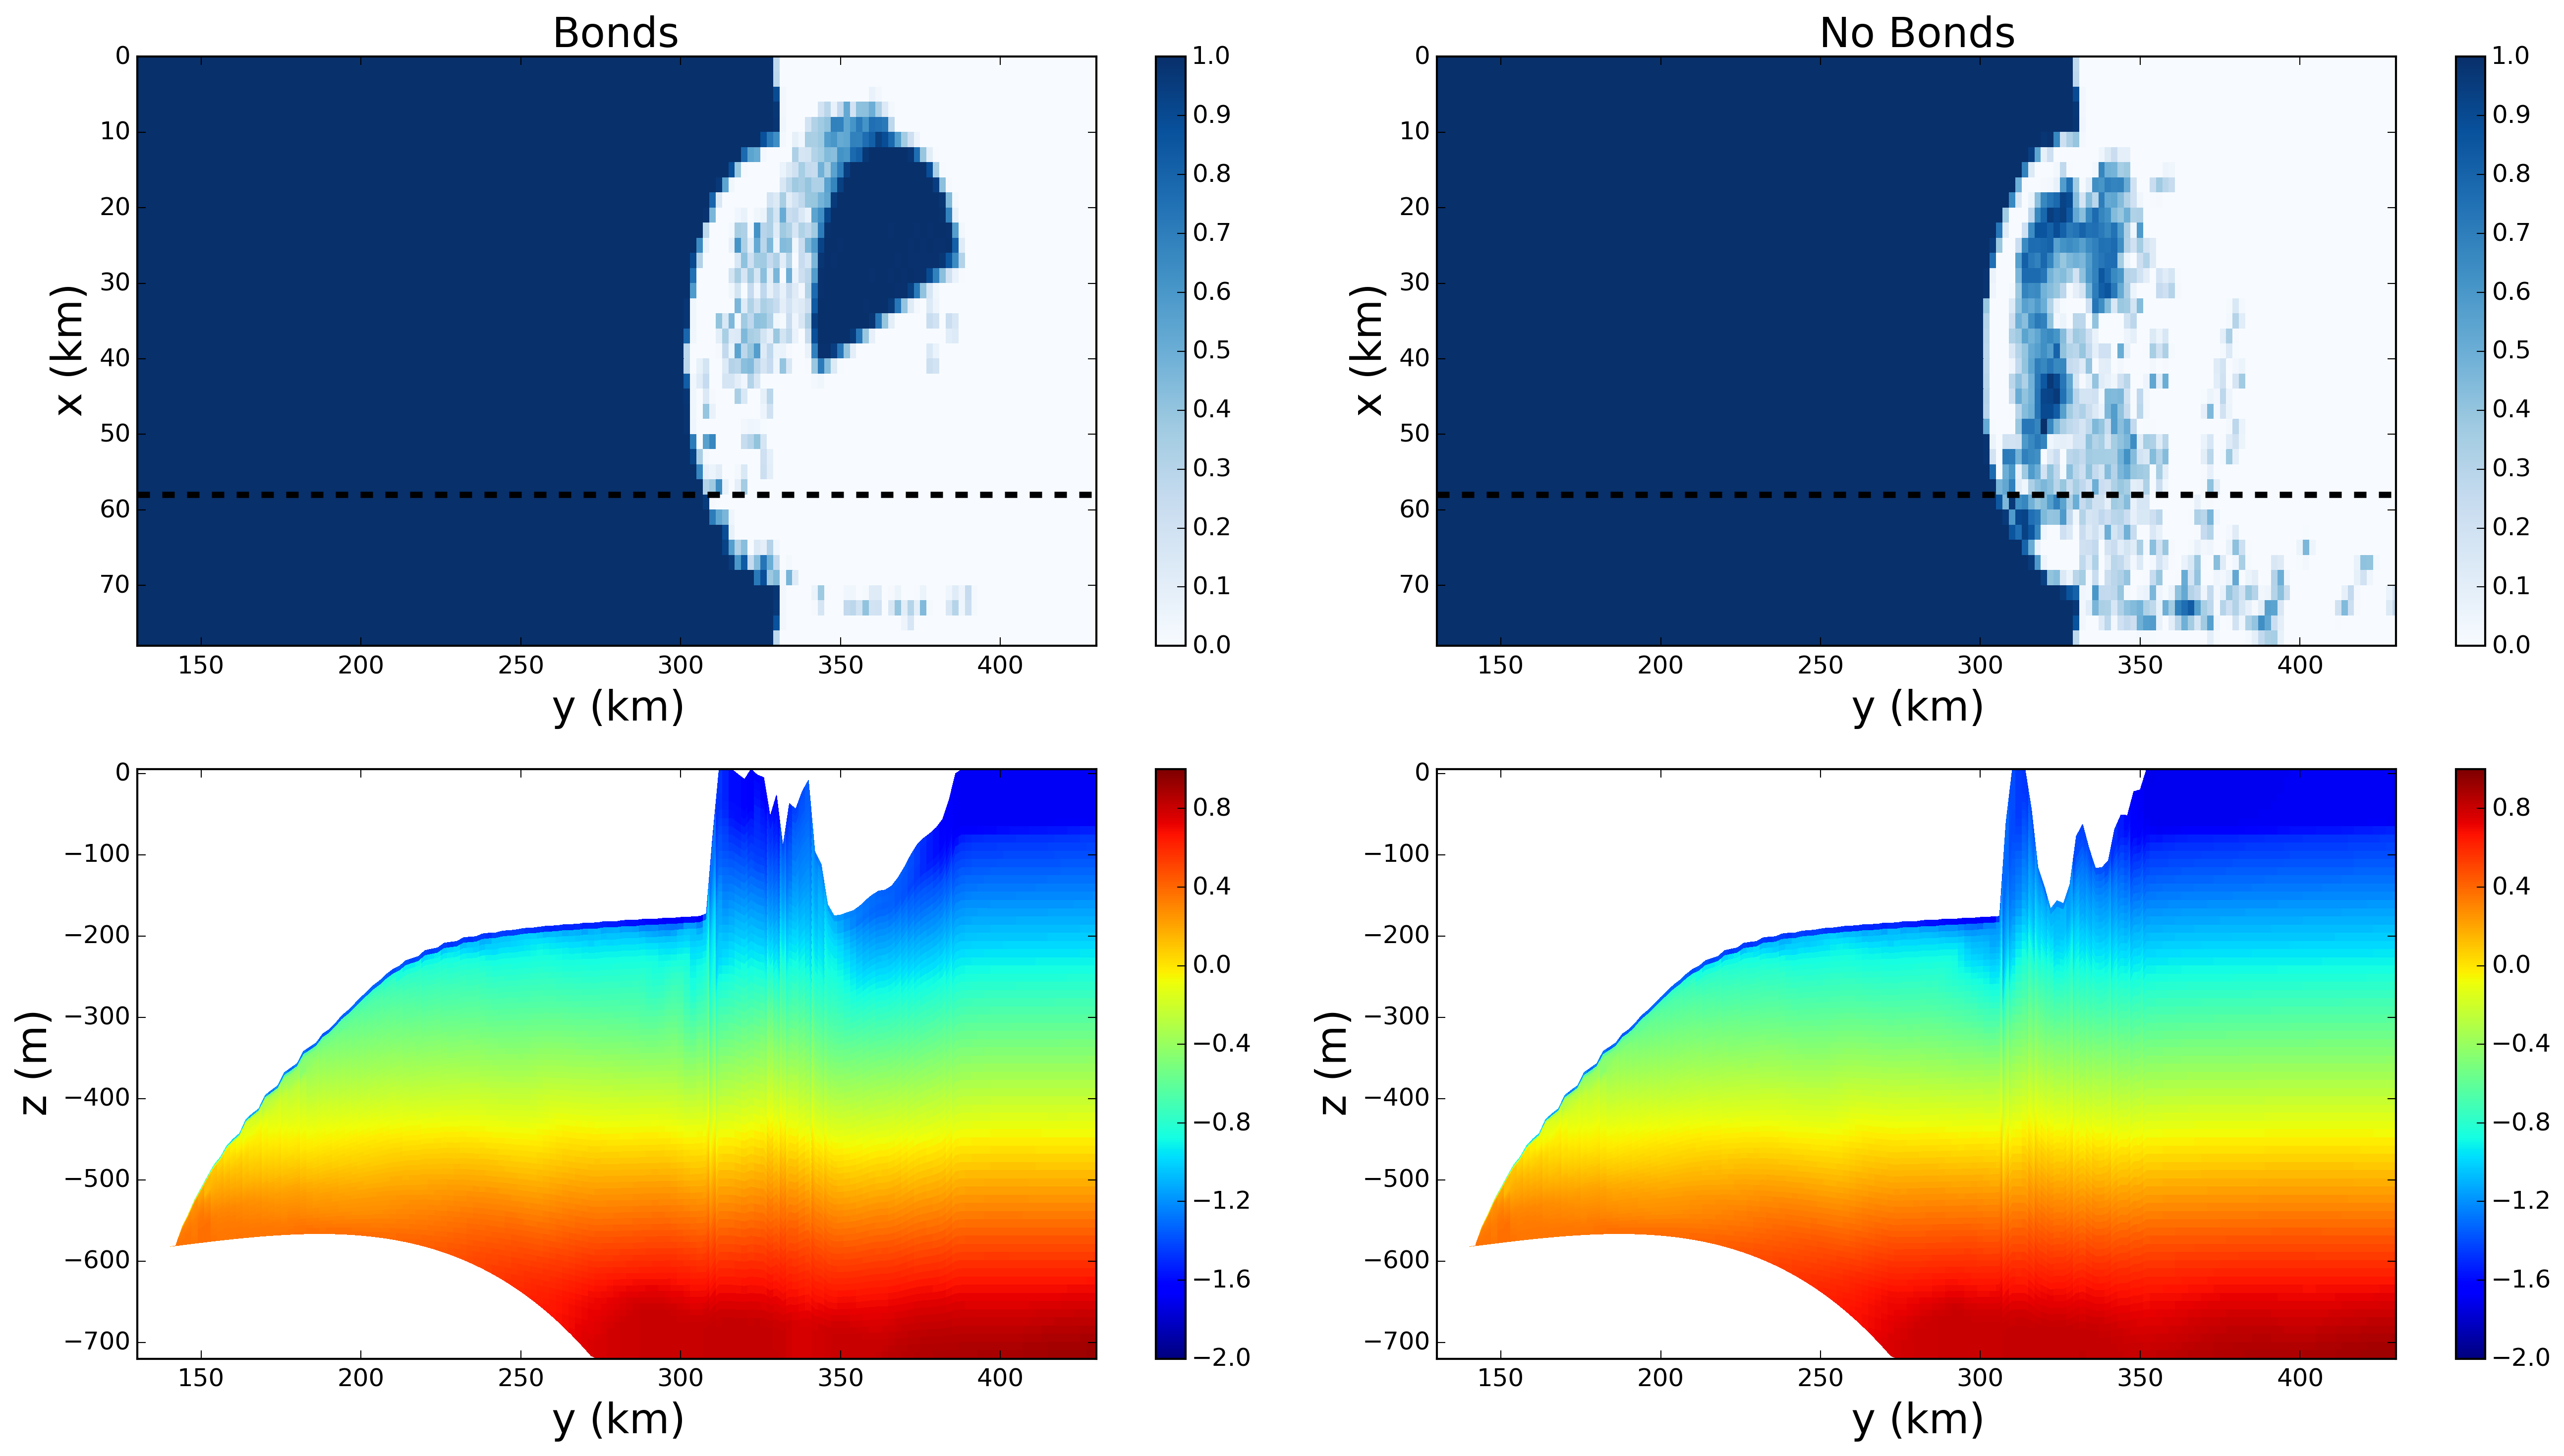
\includegraphics[width=0.99\textwidth]{/Users/alon/Desktop/files/Icebergs_clusters/Towards_Publication/Tech_paper/Github_stuff/Tech-paper/Figures/drift_bond_temp_layers.png}
%\caption{ {Results from the tabular iceberg calving experiment with and without iceberg bonds. The top row shows the fractional ice cover for the simulations (a) with and (b) without numerical bonds. The bottom row shows the corresponding vertical temperature section at $x$=54~km for the simulation (c) with and (d) without bonds. The location of the vertical transects in panels (c) and (d) are shown by the dashed lines in panels (a) and (b), respectively. All snapshots are taken at time t = 30 days. The simulations use wind stress $\vec{\tau}=< 0.0, 0.05 >.$}
%\label{fig:Bond_vs_No_bond}}
%\end{center}
%\end{figure}




 %\end{article}
 \clearpage 
%\section{Extra Figure:}
% \clearpage 
\begin{figure}
\begin{center}
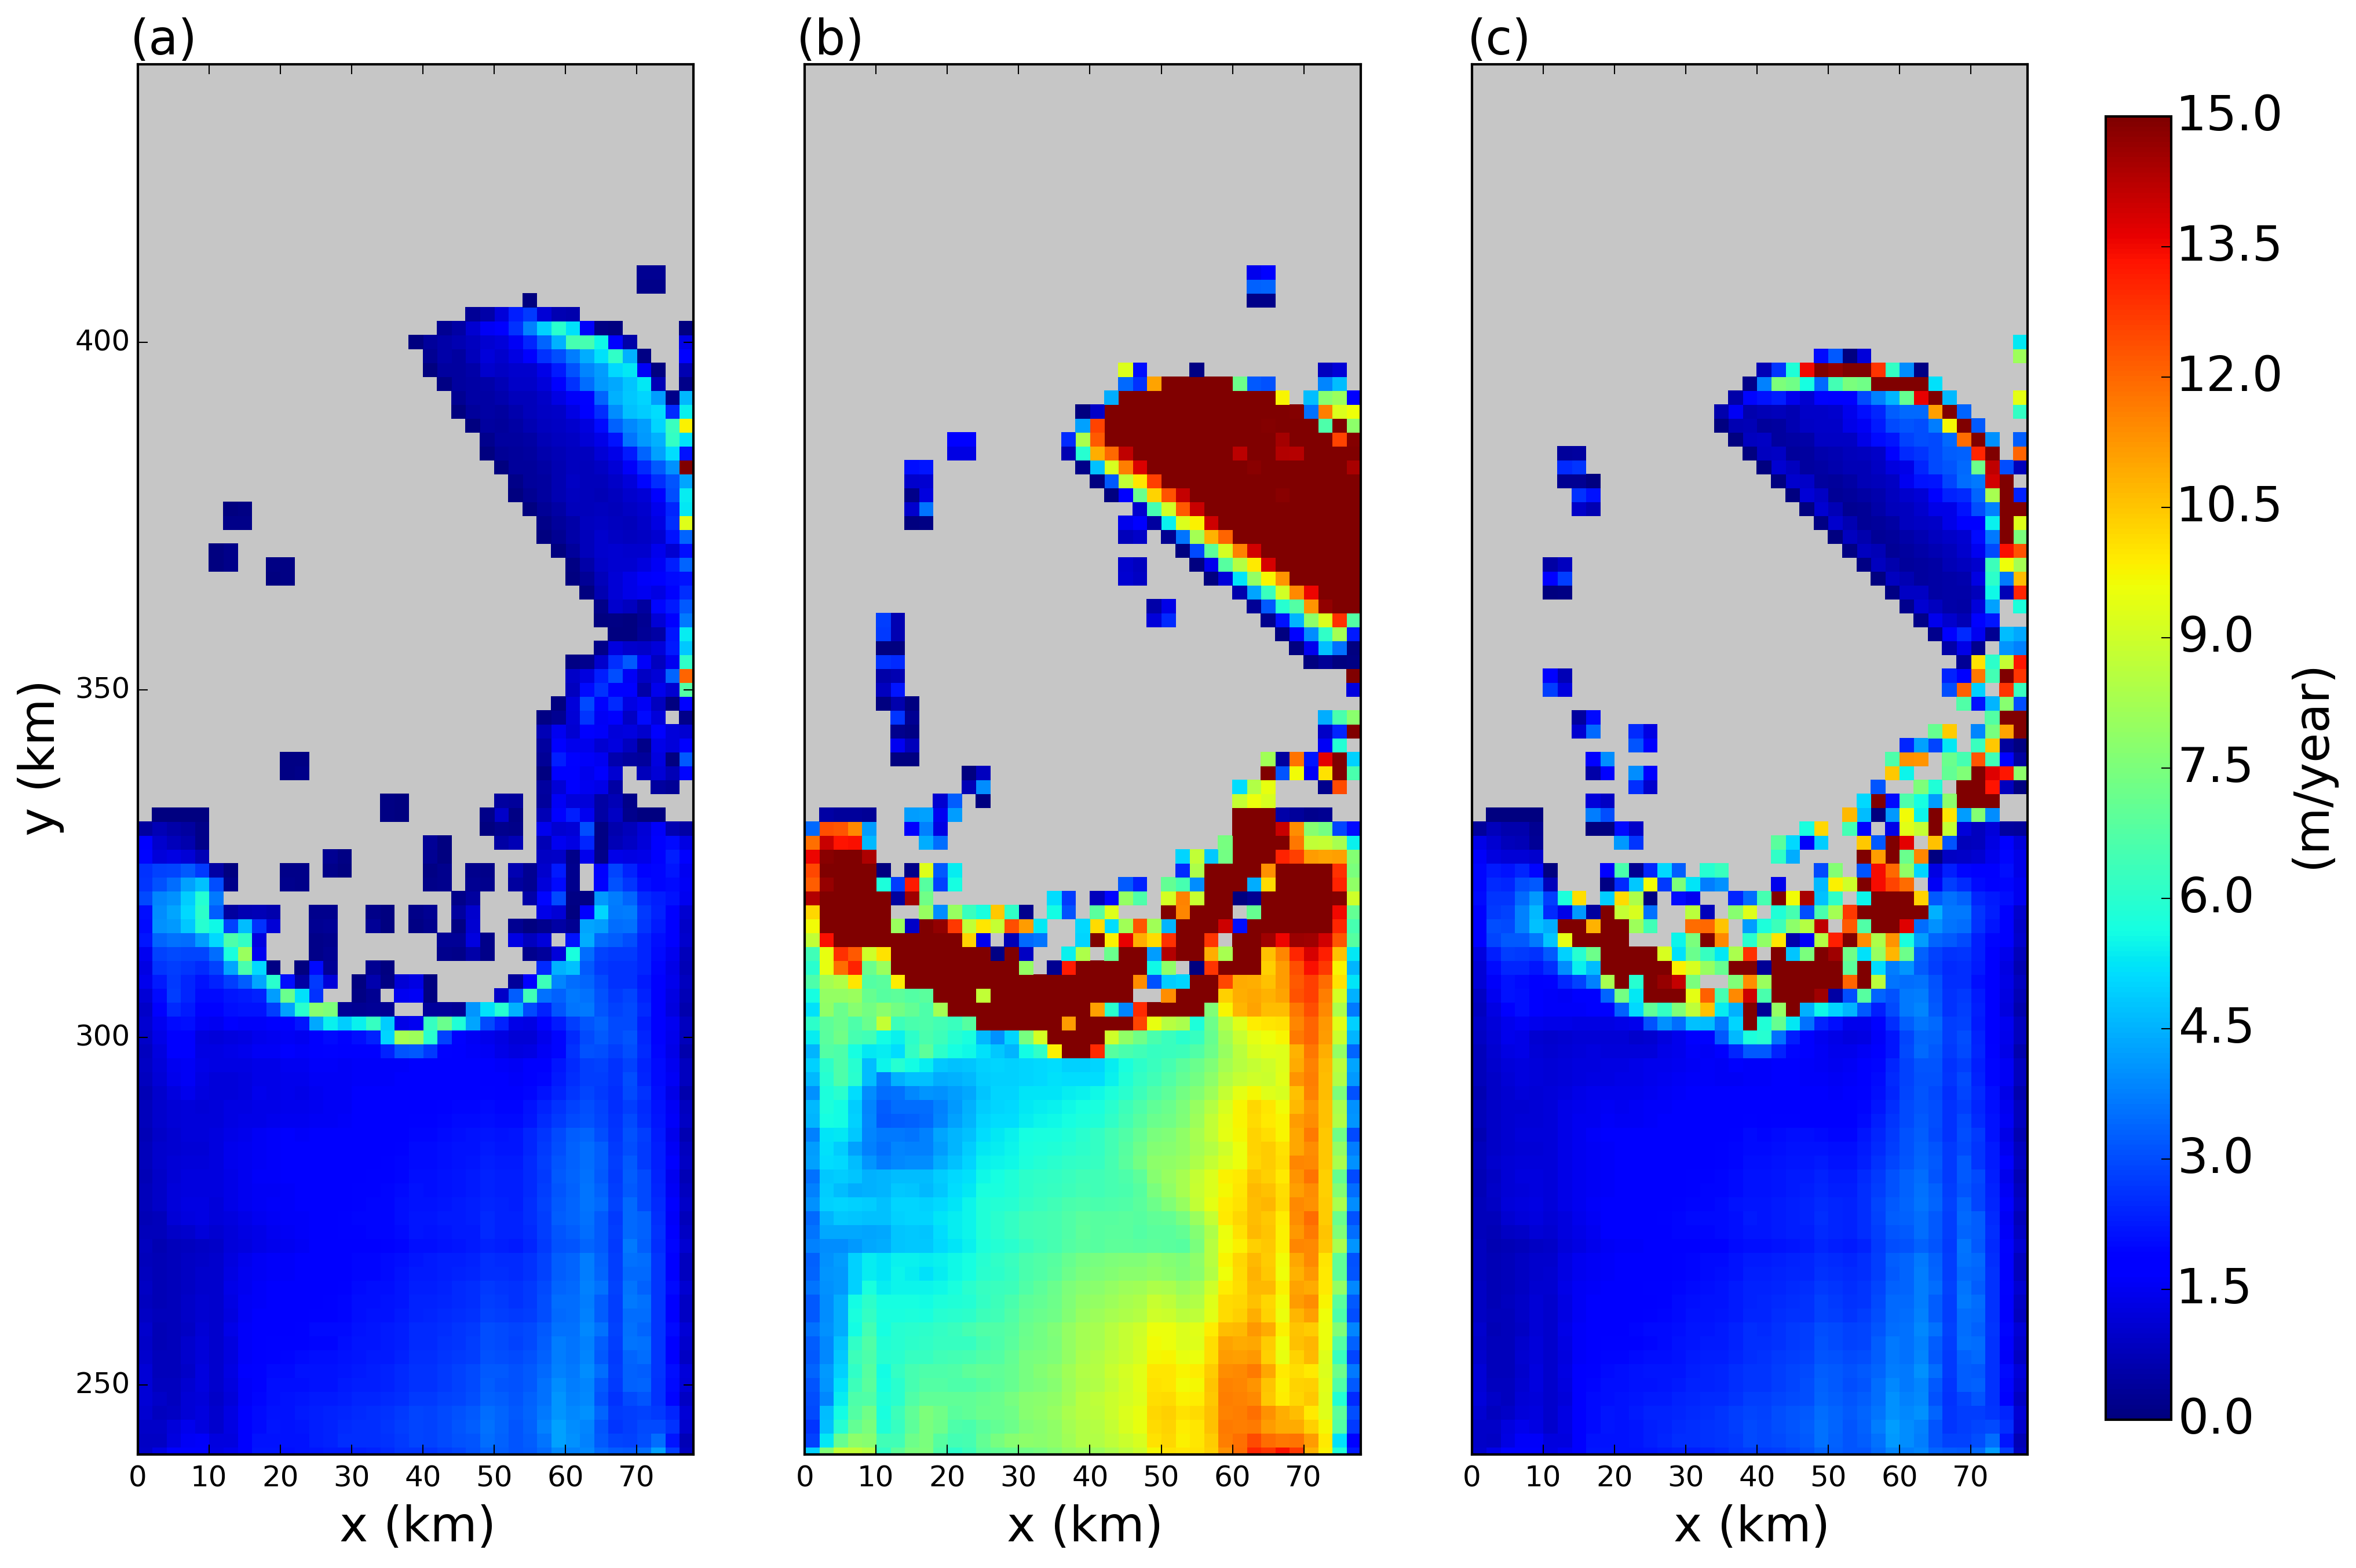
\includegraphics[width=0.99\textwidth]{/Users/alon/Desktop/files/Icebergs_clusters/Towards_Publication/Tech_paper/Github_stuff/Tech-paper/Figures/three_melt_melt_m_per_year.png}
\caption{ {Results of the tabular-iceberg-calving experiment using three different melt-rate parametrization. Panels show snapshots of the melt rate 30 days after calving for simulations using the (a) three-equation melt-rate  parametrization, (b) icebergs-drift melt-rate parametrization, (c) mixed-melt-rate parametrization (as described in Section 2.5.). Ocean grid cells without ice are masked out in grey.}
\label{fig:threemelt}}
\end{center}
\end{figure}
 \clearpage
 
 

 
 
%Text here ===>>>

%%

%  Numbered lines in equations:
%  To add line numbers to lines in equations,
%  \begin{linenomath*}
%  \begin{equation}
%  \end{equation}
%  \end{linenomath*}



%% Enter Figures and Tables near as possible to where they are first mentioned:
%
% DO NOT USE \psfrag or \subfigure commands.
%
% Figure captions go below the figure.
% Table titles go above tables;  other caption information
%  should be placed in last line of the table, using
% \multicolumn2l{$^a$ This is a table note.}
%
%----------------
% EXAMPLE FIGURE
%
% \begin{figure}[h]
% \centering
% when using pdflatex, use pdf file:
% \includegraphics[width=20pc]{figsamp.pdf}
%
% when using dvips, use .eps file:
% \includegraphics[width=20pc]{figsamp.eps}
%
% \caption{Short caption}
% \label{figone}
%  \end{figure}
%
% ---------------
% EXAMPLE TABLE
%
% \begin{table}
% \caption{Time of the Transition Between Phase 1 and Phase 2$^{a}$}
% \centering
% \begin{tabular}{l c}
% \hline
%  Run  & Time (min)  \\
% \hline
%   $l1$  & 260   \\
%   $l2$  & 300   \\
%   $l3$  & 340   \\
%   $h1$  & 270   \\
%   $h2$  & 250   \\
%   $h3$  & 380   \\
%   $r1$  & 370   \\
%   $r2$  & 390   \\
% \hline
% \multicolumn{2}{l}{$^{a}$Footnote text here.}
% \end{tabular}
% \end{table}

%% SIDEWAYS FIGURE and TABLE 
% AGU prefers the use of {sidewaystable} over {landscapetable} as it causes fewer problems.
%
% \begin{sidewaysfigure}
% \includegraphics[width=20pc]{figsamp}
% \caption{caption here}
% \label{newfig}
% \end{sidewaysfigure}
% 
%  \begin{sidewaystable}
%  \caption{Caption here}
% \label{tab:signif_gap_clos}
%  \begin{tabular}{ccc}
% one&two&three\\
% four&five&six
%  \end{tabular}
%  \end{sidewaystable}

%% If using numbered lines, please surround equations with \begin{linenomath*}...\end{linenomath*}
%\begin{linenomath*}
%\begin{equation}
%y|{f} \sim g(m, \sigma),
%\end{equation}
%\end{linenomath*}

%%% End of body of article

%%%%%%%%%%%%%%%%%%%%%%%%%%%%%%%%
%% Optional Appendix goes here
%
% The \appendix command resets counters and redefines section heads
%
% After typing \appendix
%
%\section{Here Is Appendix Title}
% will show
% A: Here Is Appendix Title
%
%\appendix
%\section{Here is a sample appendix}

%%%%%%%%%%%%%%%%%%%%%%%%%%%%%%%%%%%%%%%%%%%%%%%%%%%%%%%%%%%%%%%%
%
% Optional Glossary, Notation or Acronym section goes here:
%
%%%%%%%%%%%%%%  
% Glossary is only allowed in Reviews of Geophysics
%  \begin{glossary}
%  \term{Term}
%   Term Definition here
%  \term{Term}
%   Term Definition here
%  \term{Term}
%   Term Definition here
%  \end{glossary}

%
%%%%%%%%%%%%%%
% Acronyms
%   \begin{acronyms}
%   \acro{Acronym}
%   Definition here
%   \acro{EMOS}
%   Ensemble model output statistics 
%   \acro{ECMWF}
%   Centre for Medium-Range Weather Forecasts
%   \end{acronyms}

%
%%%%%%%%%%%%%%
% Notation 
%   \begin{notation}
%   \notation{$a+b$} Notation Definition here
%   \notation{$e=mc^2$} 
%   Equation in German-born physicist Albert Einstein's theory of special
%  relativity that showed that the increased relativistic mass ($m$) of a
%  body comes from the energy of motion of the body—that is, its kinetic
%  energy ($E$)—divided by the speed of light squared ($c^2$).
%   \end{notation}




%%%%%%%%%%%%%%%%%%%%%%%%%%%%%%%%%%%%%%%%%%%%%%%%%%%%%%%%%%%%%%%%
%
%  ACKNOWLEDGMENTS
%
% The acknowledgments must list:
%
% •	All funding sources related to this work from all authors
%
% •	Any real or perceived financial conflicts of interests for any
%	author
%
% •	Other affiliations for any author that may be perceived as
% 	having a conflict of interest with respect to the results of this
% 	paper.
%
% •	A statement that indicates to the reader where the data
% 	supporting the conclusions can be obtained (for example, in the
% 	references, tables, supporting information, and other databases).
%
% It is also the appropriate place to thank colleagues and other contributors. 
% AGU does not normally allow dedications.





%% ------------------------------------------------------------------------ %%
%% Citations

% Please use ONLY \citet and \citep for reference citations.
% DO NOT use other cite commands (e.g., \cite, \citeyear, \nocite, \citealp, etc.).


%% Example \citet and \citep:
%  ...as shown by \citet{Boug10}, \citet{Buiz07}, \citet{Fra10},
%  \citet{Ghel00}, and \citet{Leit74}. 

%  ...as shown by \citep{Boug10}, \citep{Buiz07}, \citep{Fra10},
%  \citep{Ghel00, Leit74}. 

%  ...has been shown \citep [e.g.,][]{Boug10,Buiz07,Fra10}.



%%  REFERENCE LIST AND TEXT CITATIONS
%
% Either type in your references using
%
% \begin{thebibliography}{}
% \bibitem[{\textit{Kobayashi et~al.}}(2003)]{R2013} Kobayashi, T.,
% Tran, A.~H., Nishijo, H., Ono, T., and Matsumoto, G.  (2003).
% Contribution of hippocampal place cell activity to learning and
% formation of goal-directed navigation in rats. \textit{Neuroscience}
% 117, 1025--1035.
%
% \bibitem{}
% Text
% \end{thebibliography}
%
%%%%%%%%%%%%%%%%%%%%%%%%%%%%%%%%%%%%%%%%%%%%%%%
% Or, to use BibTeX:
%
% Follow these steps
%
% 1. Type in \bibliography{<name of your .bib file>} 
%    Run LaTeX on your LaTeX file.
%
% 2. Run BiBTeX on your LaTeX file.
%
% 3. Open the new .bbl file containing the reference list and
%   copy all the contents into your LaTeX file here.
%
% 4. Run LaTeX on your new file which will produce the citations.
%
% AGU does not want a .bib or a .bbl file. Please copy in the contents of your .bbl file here.


%% After you run BibTeX, Copy in the contents of the .bbl file here:


%%%%%%%%%%%%%%%%%%%%%%%%%%%%%%%%%%%%%%%%%%%%%%%%%%%%%%%%%%%%%%%%%%%%%
% Track Changes:
% To add words, \added{<word added>}
% To delete words, \deleted{<word deleted>}
% To replace words, \replace{<word to be replaced>}{<replacement word>}
% To explain why change was made: \explain{<explanation>} This will put
% a comment into the right margin.

%%%%%%%%%%%%%%%%%%%%%%%%%%%%%%%%%%%%%%%%%%%%%%%%%%%%%%%%%%%%%%%%%%%%%
% At the end of the document, use \listofchanges, which will list the
% changes and the page and line number where the change was made.

% When final version, \listofchanges will not produce anything,
% \added{<word or words>} word will be printed, \deleted{<word or words} will take away the word,
% \replaced{<delete this word>}{<replace with this word>} will print only the replacement word.
%  In the final version, \explain will not print anything.
%%%%%%%%%%%%%%%%%%%%%%%%%%%%%%%%%%%%%%%%%%%%%%%%%%%%%%%%%%%%%%%%%%%%%

%%%
\listofchanges
%%%






\end{document}


%%%%%%%%%%%%%%%%%%%%%%%%%%%%%%%%%%%%%
%% Supporting Information
%% (Optional) See AGUSuppInfoSamp.tex/pdf for requirements 
%% for Supporting Information.
%%%%%%%%%%%%%%%%%%%%%%%%%%%%%%%%%%%%%



%%%%%%%%%%%%%%%%%%%%%%%%%%%%%%%%%%%%%%%%%%%%%%%%%%%%%%%%%%%%%%%

More Information and Advice:

%% ------------------------------------------------------------------------ %%
%
%  SECTION HEADS
%
%% ------------------------------------------------------------------------ %%

% Capitalize the first letter of each word (except for
% prepositions, conjunctions, and articles that are
% three or fewer letters).

% AGU follows standard outline style; therefore, there cannot be a section 1 without
% a section 2, or a section 2.3.1 without a section 2.3.2.
% Please make sure your section numbers are balanced.
% ---------------
% Level 1 head
%
% Use the \section{} command to identify level 1 heads;
% type the appropriate head wording between the curly
% brackets, as shown below.
%
%An example:
%\section{Level 1 Head: Introduction}
%
% ---------------
% Level 2 head
%
% Use the \subsection{} command to identify level 2 heads.
%An example:
%\subsection{Level 2 Head}
%
% ---------------
% Level 3 head
%
% Use the \subsubsection{} command to identify level 3 heads
%An example:
%\subsubsection{Level 3 Head}
%
%---------------
% Level 4 head
%
% Use the \subsubsubsection{} command to identify level 3 heads
% An example:
%\subsubsubsection{Level 4 Head} An example.
%
%% ------------------------------------------------------------------------ %%
%
%  IN-TEXT LISTS
%
%% ------------------------------------------------------------------------ %%
%
% Do not use bulleted lists; enumerated lists are okay.
% \begin{enumerate}
% \item
% \item
% \item
% \end{enumerate}
%
%% ------------------------------------------------------------------------ %%
%
%  EQUATIONS
%
%% ------------------------------------------------------------------------ %%

% Single-line equations are centered.
% Equation arrays will appear left-aligned.

Math coded inside display math mode \[ ...\]
 will not be numbered, e.g.,:
 \[ x^2=y^2 + z^2\]

 Math coded inside \begin{equation} and \end{equation} will
 be automatically numbered, e.g.,:
 \begin{equation}
 x^2=y^2 + z^2
 \end{equation}


% To create multiline equations, use the
% \begin{eqnarray} and \end{eqnarray} environment
% as demonstrated below.
\begin{eqnarray}
  x_{1} & = & (x - x_{0}) \cos \Theta \nonumber \\
        && + (y - y_{0}) \sin \Theta  \nonumber \\
  y_{1} & = & -(x - x_{0}) \sin \Theta \nonumber \\
        && + (y - y_{0}) \cos \Theta.
\end{eqnarray}

%If you don't want an equation number, use the star form:
%\begin{eqnarray*}...\end{eqnarray*}

% Break each line at a sign of operation
% (+, -, etc.) if possible, with the sign of operation
% on the new line.

% Indent second and subsequent lines to align with
% the first character following the equal sign on the
% first line.

% Use an \hspace{} command to insert horizontal space
% into your equation if necessary. Place an appropriate
% unit of measure between the curly braces, e.g.
% \hspace{1in}; you may have to experiment to achieve
% the correct amount of space.


%% ------------------------------------------------------------------------ %%
%
%  EQUATION NUMBERING: COUNTER
%
%% ------------------------------------------------------------------------ %%

% You may change equation numbering by resetting
% the equation counter or by explicitly numbering
% an equation.

% To explicitly number an equation, type \eqnum{}
% (with the desired number between the brackets)
% after the \begin{equation} or \begin{eqnarray}
% command.  The \eqnum{} command will affect only
% the equation it appears with; LaTeX will number
% any equations appearing later in the manuscript
% according to the equation counter.
%

% If you have a multiline equation that needs only
% one equation number, use a \nonumber command in
% front of the double backslashes (\\) as shown in
% the multiline equation above.

% If you are using line numbers, remember to surround
% equations with \begin{linenomath*}...\end{linenomath*}

%  To add line numbers to lines in equations:
%  \begin{linenomath*}
%  \begin{equation}
%  \end{equation}
%  \end{linenomath*}



